\documentclass[oneside]{scrbook}
\KOMAoptions{fontsize=11pt, paper=a4}     
\KOMAoptions{DIV=13}                      

\usepackage[utf8]{inputenc}               
\usepackage[T1]{fontenc}                  
\usepackage[autostyle=true]{csquotes}     
\usepackage[varg]{txfonts}  			  %	Times-like fonts in support of mathematics
\usepackage{siunitx}   	  				  
\usepackage{enumitem}				      %	extra enumerate options

\renewcommand{\familydefault}{\rmdefault} % font to sans serif

%import external graphics and where to find these
\usepackage{graphicx}					  
\graphicspath{{figs/}}

\RequirePackage[backend=biber, style=numeric]{biblatex}
\addbibresource{refs.bib}

\usepackage{hyperref}
\RequirePackage[all]{hypcap}

%There are a number of symbols defined inside txfonts that are also defined in amsmath
% so you can just make these available again
\let\iint\relax
\let\iiint\relax
\let\iiiint\relax
\let\idotsint\relax
\usepackage{amsmath}
\usepackage{physics}
\usepackage{mathtools}
\usepackage{braket}
\usepackage{slashed} % feynman slash notation
\usepackage{simplewick} % wick contraction
\usepackage{tikz-feynman} % feynman diagrams 

% This will set fancy headings to the top of the page. The page number will be
% accompanied by the total number of pages. That way, you will know if any page
% is missing.
% If you do not want this for your document, you can just use
% ``\pagestyle{plain}``.
\usepackage{scrpage2}
\usepackage{lastpage}
\pagestyle{scrheadings}
\automark{section}
%\cfoot{\footnotesize{Page \thepage\ / \pageref*{LastPage}}}
\chead{}
\ihead{}
\ohead{\rightmark}
\setheadsepline{.4pt}

%symbols for footnotes
\usepackage[symbol]{footmisc}
\renewcommand{\thefootnote}{\fnsymbol{footnote}} % footnote mark with special symbols

% toprule and etc.
\usepackage{booktabs}

%%%%%%%%%%%%%%%%%%%%%%%%%% NEW COMMAND SECTION %%%%%%%%%%%%%%%%%%%%

%define equal
\newcommand{\defeq}{\vcentcolon =} 
\newcommand{\eqdef}{= \vcentcolon}
\newcommand{\euler}{\mathrm{e}}

%Lagrange density
\newcommand{\lag}{\mathcal{L}} 
%Hamiltonian density
\newcommand{\ham}{\mathcal{H}}

%identity matrix
\usepackage{dsfont}
\newcommand{\id}{\mathds{1}}

\newcommand{\vecnab}{\pmb{\nabla}}
\newcommand{\vecx}{\pmb{x}}
\newcommand{\vecy}{\pmb{y}}
\newcommand{\veck}{\pmb{k}}
\newcommand{\N}{\mathbb{N}}
\newcommand{\R}{\mathbb{R}}
\newcommand{\M}{\mathcal{M}}

%%%%%%%%%%%%%%%%%%%%%%%%%%%%% SETTINGS %%%%%%%%%%%%%%%%%%%%%%%%%%%%%%%%%%%%

\numberwithin{equation}{section}

%%%%%%%%%%%%%%%%%%%%%%%%%%%%%%%%%%%%%%%%%%%%%%%%%%%%%%%%%%%%%%%%%%

\title{Quantum Field Theory}
\begin{document}
\maketitle
\tableofcontents
%TODO: right now chapter 1-3 only contain summaries

\chapter{Classical field theory}
\section{Field theory in continuum}
\paragraph{Euler-Lagrange-equation}
\begin{align}
	\partial_\mu \left( \frac{\partial \lag}{\partial(\partial_\mu \phi)} \right) - \frac{\partial \mathcal{L}}{\partial \phi} = 0
\end{align}
\paragraph{momentum density}
\begin{align}
	\pi(x) = \frac{\partial \lag}{\partial \dot{\phi}(\pmb{x})}
\end{align}
\paragraph{Hamiltonian density}
\begin{align}
	\ham(\phi(\pmb{x}),\pi(\pmb{x})) = \pi(\pmb{x}) \dot{\phi}(\pmb{x}) - \lag(\phi,\partial_\mu \phi)
\end{align}
\section{Noether Theorem}
If a Lagrangian field theory has an infinitisimal symmetry, then there is an associated current $j^\mu$, which is conserved.
\begin{align}
	\partial_\mu j^\mu &= 0 \\
	j^\mu &= \frac{\partial \lag}{\partial (\partial_\mu \phi)} \Delta \phi - X^mu
\end{align}
\paragraph{Energy-momentum tensor (stress-energy tensor)} \hspace{0pt}\\
Asymmetric version
\begin{align}
	\Theta^\mu_\nu = \frac{\partial \lag}{\partial(\partial_\mu \phi)} \partial_\nu \phi - \delta^\mu_\nu \lag
\end{align}
General version
\begin{align}
	T^{\mu\nu} = \Theta^{\mu\nu} + \partial_\lambda f^{\mu\nu\lambda}
\end{align}
with $f^{\lambda\mu\nu}=-f^{\mu\lambda\nu}$ or $\partial_\mu \partial\nu f^{\lambda\mu\nu}=0$


\chapter{Klein-Gordon theory}
\paragraph{(Real) Lagrangian density}
\begin{align}
	\lag = \frac{1}{2} \partial_\mu \phi \partial^\mu \phi - \frac{m^2}{2} \phi^2
\end{align}
\paragraph{Quantization}
\begin{align}
	\begin{split}
		\left[ \phi(\pmb{x}), \phi(\pmb{x}') \right] = \left[ \pi(\pmb{x}), \pi(\pmb{x}') \right] = 0 \\
		\left[ \phi(\pmb{x}), \pi(\pmb{x}') \right] = i \delta^{(3)}(\pmb{x} - \pmb{x}')
	\end{split}
\end{align}
\paragraph{Decomposition into Fourier modes}
\begin{align}
	\phi({\pmb{x}}) &= \int \frac{\dd^3 p}{(2\pi)^3}\frac{1}{\sqrt{2E_p}} \left( a_{\pmb{p}} e^{i\pmb{p}\cdot\pmb{x}} + a_{\pmb{p}}^\dagger e^{-i \pmb{p} \cdot \pmb{x}} \right) \\
	\pi({\pmb{x}}) &= \int \frac{\dd^3 p}{(2\pi)^3}(-i)\sqrt{\frac{E_p}{2}} \left( a_{\pmb{p}} e^{i\pmb{p}\cdot\pmb{x}} - a_{\pmb{p}}^\dagger e^{-i \pmb{p} \cdot \pmb{x}} \right)
\end{align}
thus the commutation relations for ladder operators:
\begin{align}
	\left[ a_{\pmb{p}}, a_{\pmb{p}'} \right] &= \left[ a^\dagger_{\pmb{p}}, a^\dagger_{\pmb{p}'} \right] = 0 \\
	\left[ a_{\pmb{p}}, a^\dagger_{\pmb{p}'} \right] &= (2\pi)^3 \delta^{(3)}(\pmb{p}-\pmb{p}')
\end{align}
\paragraph{Hamiltonian in terms of ladder operator}
\begin{align}
	H = \int \frac{\dd^3 p}{(2\pi)^3} E_p \left( a_{\pmb{p}} a_{\pmb{p}} ^\dagger + \frac{1}{2} \left[ a_{\pmb{p}}, a_{\pmb{p}}^\dagger \right] \right)
\end{align}
\paragraph{Normlisation} it's also lorentz-invariante
\begin{align}
	\braket{p|q} = 2E_p (2\pi)^3 \delta^{(3)}(\pmb{p} - \pmb{q})
\end{align}
\section{Heisenberg-picture fields}
\paragraph{Heisenberg-picture}
\begin{align}
	\ket{\psi_H} &= e^{iHt}\ket{\psi_s (t)} \\
	O_H(t) & = e^{iHt}O_S e^{-iHt} 
\end{align}
\paragraph{Field operator}
\begin{align}
	\phi(x) = \phi({\pmb{x},t}) &= \int \frac{\dd^3 p}{(2\pi)^3}\frac{1}{\sqrt{2E_p}} \left( a_p e^{ipx} + a_{p}^\dagger e^{-i p x} \right)
\end{align}

\section{Commutations and propogators}
\paragraph{Commutations}
\begin{align}
	\left[ \phi(x), \phi(y) \right] &= D(x-y) - D(y-x)
	\begin{cases}
		= 0 & \text{if $(x-y)$ is space-like} \\
		\neq 0 & \text{otherwise}
	\end{cases} \\
	D(x-y) &= \int\frac{\dd^3p}{(2\pi)^3} \frac{1}{2E_p} e^{-ip(x-y)}
\end{align}
\paragraph{Propogator}
\begin{align}
	\braket{0 | \phi(x) \phi(y) | 0} = D(x-y)
\end{align}
\paragraph{Feynman propagator}
\begin{align}
	\begin{split}
	D_F(x-y) &= \braket{0 | T \phi(x) \phi(y) | 0} \\
			 &= \Theta(x^0 - y^0)D(x-y) + \Theta(y^0 - x^0) D(y-x)
	\end{split}\\
	D_F(x-y) &= \int \frac{\dd^4 p}{(2\pi)^4}\frac{i}{p^2-m^2+i\epsilon} e^{-ip(x-y)}
\end{align}


\chapter{Quantization of the Dirac field}
\setcounter{chapter}{3}
\section{Dirac equation}
\begin{align}
	\left(i \gamma^\mu \partial_\mu - m \right) \phi(x) = 0
\end{align}
\paragraph{Standard representation (Dirac's)}
\begin{align}
	\gamma_0 = \begin{pmatrix} \id_2 & 0 \\ 0 & -\id_2 \end{pmatrix}
	\quad
	\pmb{\gamma} = \begin{pmatrix} 0 & \pmb{\sigma} \\ -\pmb{\sigma} & 0 \end{pmatrix}
\end{align}
\paragraph{Lorentz transformation}
\begin{align}
	\Lambda = \exp(\frac{1}{2}\omega_{\mu\nu}M^{\mu\nu})
\end{align}
with $\omega$ set of parameters and $M$ the generator of Lie algebra.
\paragraph{Spinor representation}
\begin{align}
	S^{\rho\sigma} &= \frac{1}{4} \left[ \gamma^\rho, \gamma^\sigma \right] = \frac{1}{2i}\sigma^{\rho\sigma} \\
\end{align}
\paragraph{Spinor transformation}
\begin{align}
	S(\Lambda) &= \exp(\frac{1}{2} \omega_{\mu\nu}S^{\mu\nu}) \\
	\psi'_a(x) &= S_{ab}(\Lambda) \psi_b(\Lambda^{-1}x)
\end{align}
\paragraph{adjoint spinor}
\begin{align}
	\bar{\psi} = \psi^\dagger \gamma^0
\end{align}
\paragraph{Fifth gamma matrix}
\begin{align}
	\gamma^5 &\defeq i \gamma^0 \gamma^1 \gamma^2 \gamma^3 \\
	\left\{ \gamma^\mu, \gamma^5 \right\} &= 0 \\
	(\gamma^5)^2 &= \id_4
\end{align}
\paragraph{Plane wavesolutions}
\begin{align}
	\psi(x) = \begin{cases}
		u(p) e^{-ipx} & \text{positive frequency} \\
		v(p) e^{ipx} & \text{negative frequency}
	\end{cases}
\end{align}
\begin{align}
	u_s	(p) = \sqrt{E_p+m} \begin{pmatrix} \chi_s \\ \frac{\pmb{u}\cdot\pmb{p}}{E_p+m}\chi_s\end{pmatrix} e^{-ipx}
	v_s	(p) = \sqrt{E_p+m} \begin{pmatrix} \frac{\pmb{u}\cdot\pmb{p}}{E_p+m}\tilde{\chi}_s \\ \tilde{\chi}_s \end{pmatrix} e^{ipx}
\end{align}
with
\begin{align*}
	\chi_{\frac{1}{2}} = \begin{pmatrix} 1 \\ 0 \end{pmatrix} \quad x_{-\frac{1}{2}} = \begin{pmatrix} 0 \\ 1\end{pmatrix} \\
	\quad s=\pm\frac{1}{2} \quad \tilde{\chi}_s = \chi_{-s}
\end{align*}
\paragraph{Orthogonality of spinor}
\begin{align}
	\bar{u}_s(p) u_{s'}(p) &= -\bar{v}_s(p) v_{s'}(p) = 2m \delta_{ss'} \\
	\bar{u}_s(p) v_{s'}(p) &= 0
\end{align}
\paragraph{Spin sums}
\begin{align}
	\sum_{s} u_s(p)\bar{u}_s(p) &= \slashed{p} + m  \\
	\sum_{s} v_s(p)\bar{v}_s(p) &= \slashed{p} - m 
\end{align}

\section{Dirac Lagrangian and quantization}
\begin{align}
	\lag = \bar{\psi}(x) (i\slashed{\partial} - m) \psi(x)
\end{align}
\paragraph{Quantization}
\begin{align}
	\left\{ \psi_a(\pmb{x}), \psi_b^\dagger(\pmb{x}') \right\} = \delta_{ab}\delta^{(3)}(\pmb{x}-\pmb{x}') \\
	\left\{ \psi_a(\pmb{x}), \psi_b(\pmb{x}') \right\} = \left\{ \psi^\dagger_a(\pmb{x}), \psi^\dagger_b(\pmb{x}') \right\} = 0
\end{align}
\paragraph{Field operators}
\begin{align}
\psi(\pmb{x}) = \int \frac{\dd^3 p}{(2\pi)^3 \sqrt{2E_p}} \sum_s (a_{\pmb{p}}^s u_s(\pmb{p})e^{i\pmb{p}\cdot\pmb{x}} + b_{\pmb{p}}^{s\,\dagger} v_s(\pmb{p})e^{-i\pmb{p}\cdot\pmb{x}})
\end{align}
thus the anticommutations of ladder operators:
\begin{align*}
	\left\{ a_{\pmb{p}}^s, a_{\pmb{p'}}^{s'\,\dagger} \right\} &= \left\{ b_{\pmb{p}}^s, b_{\pmb{p'}}^{s'\,\dagger} \right\}= (2\pi)^3\delta_{ss'}\delta^{(3)}(\pmb{p}-\pmb{p}') \\
	\left\{ a, a \right\} &= \left\{ a^\dagger, a^\dagger \right\} = \dots = 0
\end{align*}
\paragraph{Hamiltonian in terms of Fourier modes (with normal ordering)}
\begin{align}
	H = \int \frac{\dd^3 p}{(2\pi)^3} \sum_s E_p (a_{\pmb{p}}^{s\,\dagger}a_{\pmb{p}}^{s}-b_{\pmb{p}}^{s\,\dagger}b_{\pmb{p}}^{s})
\end{align}
\section{Particles and antiparticles}
\begin{align}
	Q &= e \int \dd^3 x \psi^\dagger(x)\psi(x) \\
	:Q: &= e \int \frac{\dd^3 p}{(2\pi)^3} \sum_s (a_{\pmb{p}}^{s\,\dagger}a_{\pmb{p}}^s - b_{\pmb{p}}^{s\,\dagger}b_{\pmb{p}}^s)
\end{align}
\section{Dirac propagator and anticommutators}
\begin{align}
	\begin{split}
	S_{ab}(x-y) &= \left\{ \psi_a(x), \bar{\psi}_b(y) \right\} \\
				&= (i\slashed{\partial}+m) \left[ D(x-y)-D(y-x) \right]
	\end{split}
\end{align}
\paragraph{Time ordering of Dirac fields}
\begin{align}
	T(\phi_a(x)\bar{\psi}_b(y)) = \Theta(x^0 - y^0)\psi_a(x)\bar{\psi}_b(y) - \Theta(y^0 - x^0) \bar{\psi}_b(y)\psi_a(x)
\end{align}
\paragraph{Feynman propogator for the Dirac field}
\begin{align}
	S_F(x-y) = \braket{0| T \psi(x)\bar{\psi}(y) |0} = \int \frac{\dd^4 p}{(2\pi)^4} \frac{i(\slashed{p}+m)}{p^2-m^2+i\epsilon} e^{-ip\cdot(x-y)}
\end{align}

\section{Discrete symmetries of the Dirac Field}
\begin{center}
\begin{tabular}{c c c}
	\toprule
& orientation perserving & orientation not perserving \\
\midrule
	(ortho)chronous & $\mathcal{L}_+^{\uparrow}$ & $\mathcal{L}_-^\uparrow=\mathcal{P}\mathcal{L}_+^{\uparrow}$ \\
	non-orthochronous & $\mathcal{L}_-^\downarrow = \mathcal{T}\mathcal{L}_+^{\uparrow}$ & $\mathcal{L}_+^{\downarrow}=\mathcal{P}\mathcal{T}\mathcal{L}_+^{\uparrow}$ \\
	\bottomrule
\end{tabular}
\end{center}


\chapter{Interacting QFT}
\setcounter{chapter}{4}
\section{Introduction and examples}
Theories discussed so far are Klein-Gordon theory with spin $0$ 
$$\lag_{KG} = \frac{1}{2}\partial_\mu\phi\partial^\mu\phi - \frac{m^2}{2}\phi^2$$ 
and Dirac theory spin $\frac{1}{2}$ 
$$\lag_D = \bar{\psi}(i\slashed{\partial} - m) \psi $$

There is also $\lag_{EM} = -\frac{1}{4}F_{\mu\nu}F^{\mu\nu}$ with $F_{\mu\nu} = \partial_\mu A_\nu - \partial_\nu A_\mu$ for a massless vector filed. Its quantiasation gives photon.

One thing they have in common is quadratic in the fields. As result:
\begin{itemize}
	\item linear field equations
	\item exact quantisation
	\item multi-particle states without scattering or interaction
	\item linear fourier decompositions , no mementum changes
\end{itemize}

To have an interacting theory with scattering, need higher powers in the field in the Lagrangians. A few examples are following
\paragraph{Scalar $\phi^4$ theory}
\begin{align*}
	\lag = \lag_{KG} + \frac{\lambda}{4!} \phi^4
\end{align*}
need positive sign $\lambda > 0$ for a stable theory, otherwise classical energy can be arbitarily negative.

Equation of motions
\begin{align*}
	(\partial^2+ m ^2) \phi = -\frac{\lambda}{3!} \phi^3
\end{align*}
is nonlinear, cannot be solved by Fourier decomposition.

\paragraph{Yukawa-theory}
\begin{align*}
	\lag = \lag_{KG} + \lag_{D} - g \bar{\psi}\psi \phi
\end{align*}
It is originally developed as a theory for nuclear forces with $\psi$ nucleon, $\phi$ pion. In the Standard Model it is similar to interactions in Higgs mechanism.
\paragraph{Quantum Electrodynamics (QED)}
\begin{align*}
	\lag = \lag_{EM} + \lag_{D} - eA_\mu \bar{\psi} \gamma^\mu \psi
\end{align*}
descreibes electrons, their antiparticles positrons and photons.

\paragraph{Yang-Mills theory}
generalises $\lag_{EM}$ with terms like $A^4$ or $A^2 \partial A$
\paragraph{Scalar QED}
descreibes pions and photons
\begin{align*}
	\begin{split}
		\lag &= \lag_{EM} + D_\mu \phi D^\mu\phi^* - m^2 |\phi|^2 \\
			 &= \lag_{EM} + \partial_\mu\phi\partial^\mu\phi^* - m^2 \phi\phi^* + ie A_\mu(\phi\partial^\mu\phi^* - \phi^* \partial^\mu\phi) + e^2 A_\mu A^\mu \phi\phi^*
	\end{split}
\end{align*}
\paragraph{Remarks}
\begin{enumerate}
	\item Interaction terms in $H_\text{int} = \int \dd^3x \ham_\text{int} = - \int\dd^3x\lag_\text{int}$ always involves products of fields at the same point $\pmb{x}$. It ensures causality, no "instant at a distance".
	\item There are no derivative interactions. These may complicate quantisation as $$\pi(\pmb{x}) = \frac{\partial\lag}{\partial(\partial_0 \phi(\pmb{x}))}$$
	\item Why are we taking the examples above? There must be zillions of theories (Lagrangians)? \\
			We have the criterion of \textbf{renormalizability}. Note the mass dimensions of fields;
			\begin{align*}
				[S] = 1 \, \text{so} \, [\lag] = [M]^4 \, \Rightarrow [\phi] = [M] ,\, [\psi] = [M]^{\frac{3}{2}} ,\, [A_\mu] = [M]
			\end{align*}
			So in all the interaction terms indicated above, the coupling constant $\lambda$, e, g are all \textbf{dimensionless}!\\
			Can add $-\frac{\mu}{3!}\phi^3$ to the $\phi^4$ theory. This leads to $[\mu] = [M]$ and all these generate renormalisable interactions. \\
			All higher interaction terms require coupling constants of \textbf{negative} mass dimension, e.g. $G\bar{\psi}\psi\bar{\psi}\psi$ and then $[G] = [M]^{-2}$. These are nonrenormalisable and create trouble when performing higher-order calculation in perturbation theory.
			(with energy cutoff; corrections $~G\Lambda^2$, $\Lambda \rightarrow \infty$)
		\item we haven't quantised the photon yet. The reason is that its is a vector field, i.e. 4 degrees of freedom, but photon has just $2$ physical polarisaion states. It is linked to gauge symmetry and complicates quantisation somewhat.
\end{enumerate}
\section{The interaction picture}
Consider the $\phi^4$ theory, 
\begin{align}
\lag_{int} = -\frac{\lambda}{4!} \phi(x)^4
\end{align}
Hamiltonian $H = H_0 + H_{int}$ with 
\begin{align}
	H_0 &= \int\dd^3 x \left\{ \frac{1}{2}\pi^2(x) + \frac{1}{2}(\pmb{\nabla}\phi)^2 + \frac{1}{2}m^2\phi^2 \right\}\\
	H_{int} &= -\int\dd^3x \lag_{int} = \frac{\lambda}{4!}\int\dd^3x \phi^4 
\end{align}

Interaction picture means that operators evolve in time using $H_0$ (only), in particular 
\begin{align}
	\phi_I(t,\pmb{x}) = e^{iH_0t}\phi(\pmb{x})e^{-iH_0t}
\end{align}

Time-dependence of the free field, obeys classical equation of motion $\left(\partial^2+m^2 \right)\phi_I(t,\pmb{x}) = 0$. Solution in terms if fourier modes as before:
\begin{align}
	\phi_I = \int \frac{\dd^3 p}{(2\pi)^3\sqrt{2E_p}} (a^I_{\pmb{p}}e^{-ipx} + a^{I\,\dagger}_{\pmb{p}}e^{+ipx})
\end{align}
as in the free theory with standard commutation relations $[a^I_{\pmb{p}}, a^{I\,\dagger}_{\pmb{p}}] = (2\pi)^3\delta^{(3)}(\pmb{p}-\pmb{p}')$. The state satisfing $a^I_p \ket{0} = 0$ is the vacuum of the free, noninteratcting theory.

Relation between interaction and Schrödinger picure states:
\begin{align}
	\ket{\phi_I(t)} = e^{iH_0t}{\ket{\psi_S(t)}}
\end{align}
Schrödinger equation becomes: 
\begin{align}
	i\frac{\partial}{\partial t}\ket{\psi_S} &= (H_0 + H_\text{int})\ket{\psi_S} \notag\\
	\text{LHS} &= i \frac{\partial}{\partial t} \left( e^{-iH_0t}\ket{\phi_I} \right) = H_0 e^{-iH_0t}\ket{\phi_I} + e^{-iH_0t}i\frac{\partial}{\partial t}\ket{\phi_I} \notag\\
	\text{RHS}														&= \left(H_0 + H_\text{int}\right)e^{-iH_0t}\ket{\phi_I} \notag\\
	\Rightarrow i\frac{\partial}{\partial t}\ket{\phi_I} &= e^{iH_0t}H_{int} e^{-iH_0t} = H_I(t)\ket{\phi_I} \label{math:int-schr}
\end{align}
with $H_I$ interaction Hamiltonian in the interaction picture. Clearly
\begin{align}
	H_I = \frac{\lambda}{4!}\int\dd^3x\phi_I^4(x) \notag
\end{align}

What is the solution of~\ref{math:int-schr} for the time evolution of $\ket{\phi_I(t)}$? Define time-evolution operator in the interaction picture.
\begin{align}
	\ket{\phi_I(t)} &= U(t,t_0)\ket{\phi_I(t_0)}\label{math:int-schr2}\\
	\text{where} \; U(t,t_0) &= e^{iH_0(t-t_0)}e^{-iH(t-t_0)} 
\end{align}

With~\ref{math:int-schr} and~\ref{math:int-schr2}:
\begin{align}
	i\frac{\partial}{\partial t} U(t,t_0) = H_I(t)U(t,t_0)
\end{align}

To solve with boundary conditions: $U(t_0, t_0) = \id$. The formal solution:
\begin{align}
	U(t,t_0) = 1 - i \int_{t_0}^t \dd t' H_I(t')U(t',t_0) \notag
\end{align}

Substitute back in and we get:
\begin{align*}
	U(t,t_0) = 1- i \int_{t_0}^t \dd t' H_I(t') + (-i)^2 \int_{t_0}^t \dd t' \int^{t'}_{t_0} \dd t'' H_I(t') H_I(t'') + \dots
\end{align*}

$H_I$ inside the integral is automatically time-ordered. Ranges of integration is not. 

\begin{figure}[ht]
	\centering
	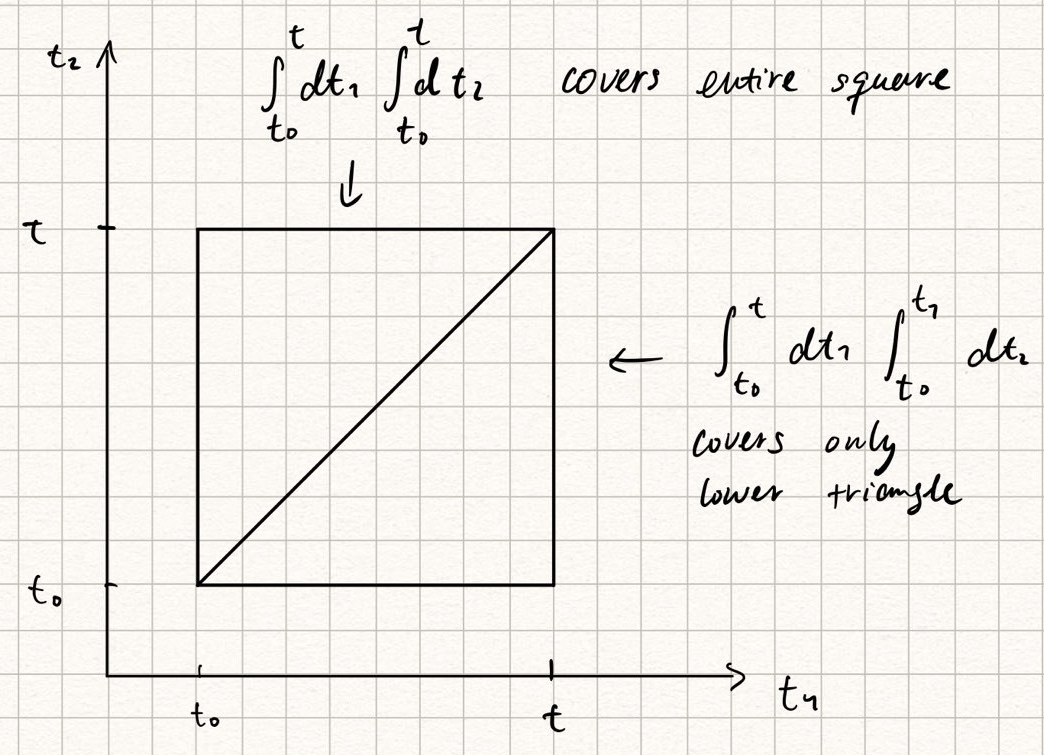
\includegraphics[width=0.65\linewidth]{4-2-triangle.jpg}
	\caption{Time ordering}
	\label{fig:4-2-triangle}
\end{figure}

Upper triangle has the wrong time order. We are going to "repair" it by hand.
\begin{align}
	U(t,t_0) &= 1-i\int_{t_0}^t \dd t' H_I(t') + \frac{(-i)^2}{2} \int_{t_0}^t \dd t' \int^{t}_{t_0} \dd t'' T(H_I(t') H_I(t'')) + \dots \notag\\
			 &= \sum_{n=0}^{\infty} \frac{(-i)^n}{n!}\int_{t_0}^t \dd t_1 \dots \int_{t_0}^t \dd t_n T(H_I(t_1) \dots H_I(t_n))  \notag\\
			 &= T \exp{-i\int_{t_0}^t \dd t' H_I(t') }
\end{align}

It is interesing for scattering to transition into asymptotic state for $t \rightarrow \infty$
\begin{align}
	S = \lim_{t \rightarrow \infty} U(t,-t) &= T \exp{-i \int_{-\infty}^\infty \dd t H_I(t)} \\
	 &\stackrel{\phi^4}{=} T \exp{-i\int \dd^4 x \frac{\lambda}{4!} \phi_I^4(x)} \notag
\end{align}
Both $U$ and $S$ are formally unitary

Composition law for time evolution operator: 
\begin{align}
	U(t_2, t_0) = U(t_2, t_1) U(t,t_0) = U(t_2, t_1) U(t_0, t_1)^\dagger
\end{align}

\subsection{Scattering amplitudes and the S-matrix}
Take $\ket{i}$ the initial (multi-particle) state and $\ket{f}$ the final (multi-particle) state. Time evolution of $\ket{i}$ then is
$$\lim(t\rightarrow\infty)U(t,-\infty) \ket{i} = S \ket{i}$$

Probability that $\ket{i}$ evolves into $\ket{f}$ is proporional to the squared "\textbf{S-matrix element}"
\begin{align}
	\left|	\braket{f,\, t\to \infty | i, t\rightarrow - \infty}\right|^2 = \left| \braket{f|S|i} \right|^2 = \left| S_{fi} \right|^2
\end{align}

The nontrivial part of the S-matrix is the T-matrix:
\begin{align}
	S_{fi} \defeq \delta_{fi} + iT_{fi}
\end{align}

Use momentum conservation (from translation invariance) to define matrix element
\begin{align}
	S_{fi} = \delta_{fi} + i(2\pi)^4 \delta^{(4)}(p_f - p_i) M_{fi}
\end{align}
$M_{fi}$ measures "genuine scattering" from $\ket{i}$ to $\ket{f}$.

How are we going to calculate correlation functions in the interacting theory:
\begin{align}
	\braket{\Omega |  \ T \phi(x)\phi(y) | \Omega}	
\end{align}
or more generally $\braket{\Omega | T \phi(x_1)\phi(x_2)\dots | \Omega}$, where $\ket{\Omega}$ is the vaccum/ground state of the interacting theory and $\phi(x)$ the Heisenberg operators?

Ignore $\ket{\Omega} \neq \ket{0}$ for the moment other than saying: we want to study the time evolution from the vacuum at $t\rightarrow - \infty$ to $t \rightarrow + \infty$. So rewriting in terms $\phi_I(x)$, assuming $x^0 > y^0$ for now:
\begin{align}
	\braket{0 | U(\infty, x^0) \phi_I(x^0)  U(x^0, y^0) \phi_I(y^0)U(y^0, -\infty) | 0}  = \braket{0|T(\phi_I(x)\phi_I(y)S)|0}
\end{align}
still holds if $x^0 < y^0$ because of $T$.

Now $\ket{\Omega} \neq \ket{0}$: this can be taken care of by dividing out the time evolution of the (free) vacuum $\braket{0|S|0}$, so
\begin{align}
	\braket{\Omega | T(\phi(x)\phi(y))|\Omega} \notag\\
	&= \frac{\braket{0 | T(\phi_I(x)\phi_I(y)S)|0}}{\braket{0|S|0}} \\
	&\stackrel{\phi^4}{=} 
	\frac{\braket{0 | T {\phi_I(x)\phi_I(y)\exp{-i\int\dd^4x' \frac{\lambda}{4!}\phi^4(x')}}| 0}}
	{\braket{0 | T {\exp{-i\int\dd^4x' \frac{\lambda}{4!}\phi^4(x')}}| 0}
}\notag
\end{align}
Proof can be found in Peskin. It will also be illustrated parctically later ("vacuum bubbles").

Perturbation theory is viable when $\lambda$ (or some other coupling) is "small" and then expands $U(t,t_0)$ or $S$ in powers of $\lambda$.

\section{Wick's theorem}
From now on drop the subscript for interaction pictire fields $\phi_I(x) \rightarrow \phi(x)$.

Want to calculate stuff like $\braket{0 | T\phi(x_1)\dots\phi(x_n)S | 0}$ in perturbation theory; so e.g.\ at order $\lambda^n$. So 
\begin{align}
\frac{1}{n!} \left( -i\frac{\lambda}{4!} \right)^n \int \dd^4 y_1 \dots \dd^4 y_n \braket{0 | T\phi(x_1)\dots\phi(x_n)\phi^4(y_1)\dots\phi^4(y_n) | 0}
\end{align}
is tough!

We know $\braket{0 | T\phi(x_1)\phi(x_2) | 0 } $ is the Feynman propagator!

Recall \textbf{normal ordering} with $\phi(x) = \phi^+(x) + \phi^-(x)$
\begin{align}
	:\phi^+ \phi^-: = :\phi^- \phi^+: = \phi^- \phi^+
\end{align} 
where
\begin{align*}
\phi^+ &= \int \frac{\dd^3 p}{(2\pi)^3} \frac{1}{\sqrt{2E_{\pmb{p}}}} a_{\pmb{p}} e^{-ip\cdot x} \\
	\phi^- &= \int \frac{\dd^3 p}{(2\pi)^3} \frac{1}{\sqrt{2E_{\pmb{p}}}} a^\dagger_{\pmb{p}} e^{+ip\cdot x}
\end{align*}
Wick's therem expresses time-ordered products in terms of normal-ordered ones. Then it is easy to take vacuum expectation values, as $\braket{0 | :\phi(x_1)\dots\phi(x_n):|0} = 0$

Take two fields and $x^0 > y^0$:
\begin{align*}
	T \phi(x)\phi(y) &= \phi(x)\phi(y) = \left(\phi^+(x)+\phi^-(x)\right)\left(\phi^+(y)+\phi^-(y)\right) \\
	&= \phi^+(x)\phi^+(y) + \phi^-(x)\phi^-(y) + \phi^-(x) \phi^+(y) + \phi^-(x) \phi^+(y) + [\phi^+(x), \phi^-(y)] \\
	&= :\phi(x)\phi(y): + [\phi^+(x),\phi^-(y)]
\end{align*} 

Particularly for $y^0 > x^0$: 
\begin{align}
	T\phi(x)\phi(y) = :\phi(x)\phi(y): + [\phi^+(y),\phi^-(x)] \notag
\end{align}

Thus altogether: 
\begin{align}
	T\phi(x)\phi(y) = :\phi(x)\phi(y): + D_f(x-y)
\end{align}
as $\Theta(x^0 - y^0) [\phi^+(x), \phi^-(y)] + \Theta(y^0 - x^0) [\phi^+(y), \phi^-(x)] = D_F(x-y)$.

Worth noting that $D_F(x-y)$ is still a c-number, not operator (yet). Thus it can be pulled out of any matrix element or expectation value.

We now define "contraction":
\begin{align}
	\contraction[1ex]{}{\phi}{(x_1)}{\phi}	\phi(x_1) \phi(x_2) = D_F(x_1-x_2)
\end{align}

Thus we can remove the fields from the product leaving only the propagators:
\begin{align}
	T\phi(x)\phi(y) = :\phi(x)\phi(y): +  \contraction[1ex]{}{\phi}{(x)}{\phi}	\phi(x) \phi(y)
\end{align}

General form of \textbf{Wick's theorem} for arbitary number of fields
\begin{align}
	T\phi(x_1)\dots \phi(x_n) = :\phi(x_1)\dots \phi(x_n):	 + :\left( \text{sum over all possible contractions} \right):
\end{align}

Example with four fields:
\begin{align*}
	T(\phi_1 \phi_2 \phi_3 \phi_4) &= :\phi_1 \phi_2 \phi_3 \phi_4: \\
								   & + \contraction{}{\phi_1}{}{\phi_2} \phi_1 \phi_2 :\phi_3 \phi_4: + \contraction{}{\phi_1}{}{\phi_3} \phi_1 \phi_3 :\phi_2 \phi_4: + \contraction{}{\phi_1}{}{\phi_4} \phi_1 \phi_4 :\phi_2 \phi_3: +  \contraction{}{\phi_2}{}{\phi_3} \phi_2 \phi_3 :\phi_1 \phi_4: + \contraction{}{\phi_2}{}{\phi_4} \phi_2 \phi_4 :\phi_1 \phi_3: + \contraction{}{\phi_3}{}{\phi_4} \phi_3 \phi_4 :\phi_1 \phi_2: \\
	&+ \contraction{}{\phi_1}{}{\phi_2} \phi_1 \phi_2 \contraction{}{\phi_3}{}{\phi_4}\phi_3 \phi_4 + \contraction{}{\phi_1}{}{\phi_3} \phi_1 \phi_3 \contraction{}{\phi_2}{}{\phi_4}\phi_2 \phi_4 + \contraction{}{\phi_1}{}{\phi_4} \phi_1 \phi_4 \contraction{}{\phi_2}{}{\phi_3}\phi_2 \phi_3
\end{align*}

Thus 
\begin{align*}
	\braket{0 | T \left(\phi_1 \phi_2 \phi_3 \phi_4 \right) | 0} = D_F (x_1 - x_2) D_F(x_3 - x_4) + D_F (x_1 - x_3) D_F(x_2 - x_4) + D_F (x_1 - x_4) D_F(x_2 - x_3) 
\end{align*}
which can be visually represented as
\begin{center}
\begin{tikzpicture}[scale=1, transform shape]
	\begin{feynman}
		\vertex (x1) {$x_1$};
		\vertex [below=of x1] (x2) {$x_2$};
		\vertex [right=of x1] (x3) {$x_3$};
		\vertex [below =of x3] (x4) {$x_4$};
		\diagram*{
			(x1) -- (x2),
			(x3) -- (x4),
		};
	\end{feynman}	
\node at (2,-0.8) {$+$};
\end{tikzpicture}
\begin{tikzpicture}[scale=1, transform shape]
	\begin{feynman}
		\vertex (x1) {$x_1$};
		\vertex [below=of x1] (x2) {$x_2$};
		\vertex [right=of x1] (x3) {$x_3$};
		\vertex [below =of x3] (x4) {$x_4$};
		\diagram*{
			(x1) -- (x3),
			(x2) -- (x4),
		};
	\end{feynman}	
\node at (2,-0.8) {$+$};
\end{tikzpicture}
\begin{tikzpicture}[scale=1, transform shape]
	\begin{feynman}
		\vertex (x1) {$x_1$};
		\vertex [below=of x1] (x2) {$x_2$};
		\vertex [right=of x1] (x3) {$x_3$};
		\vertex [below =of x3] (x4) {$x_4$};
		\diagram*{
			(x1) -- (x4),
			(x3) -- (x2),
		};
	\end{feynman}	
\end{tikzpicture}
\end{center}

%%%%%%%% 15.05.2019 %%%%%%%
Proof of the general theorem by \textit{induction} in the number of fields (see exercise). The idea is to suppose it is true for $\phi_2 \dots \phi_m$, $x^0_1 > x^0_{k>1}$. Then 
\begin{align*}
	T\phi_1 \phi_2 \dots \phi_m &= (\phi^+_{1} + \phi^-_{1})T\phi_2 \dots \phi_m \\
								& = (\phi^+_{1} + \phi^-_{1}) [:\phi_2 \dots \phi_m: + :\text{contractions}:]
\end{align*}
$\phi^-_1$ can stay as it is part of $(:\phi_1 \phi_2 \dots \phi_m:)$. But $\phi^+_1$ needs to be comuted past all $\phi^-_1$ operators, giving rise to additional contractions $\contraction{}{\phi_1}{}{\phi_2} \phi_1\phi_2$.

\paragraph{Consequences}
\begin{itemize}
	\item $n = 2k+1, \, k \in \N$
		\[
		\braket{0 | T \phi_1 \dots \phi_m | 0} = 0
		\]
	\item $n = 2k, \, k \in \N$	
		\[
			\braket{0 | T \phi_1 \dots \phi_m | 0} = \sum_{\text{pairing of fields}} D_F(x_{i_1}-x_{i_2})\dots D_F(x_{i_{m-1}}-x_{i_m})
		\]
\end{itemize}

\subsection{Wick's theorem and the S-Matrix}
Apply Wick's theorem to correlation functions $\braket{0 | T \{\phi_1 \dots \phi_m \} S | 0}$ n-th term in the perturbative expansion of $S$ with $\phi(x_1) \defeq \phi_1$.
\begin{align*}
	\frac{1}{n!} \left(\frac{-i\lambda}{4!}\right)^n \int \dd^4 y_1 \dots \dd^4 y_n \braket{0 | T \{ \phi_1 \dots \phi_m  \phi^4(y_1) \dots \phi^4(y_n) \} | 0}
\end{align*}

\paragraph{Example with $m=4 ,\, n=1$}
\begin{align*}
	-\frac{i\lambda}{4!} &\int \dd^4 x \braket{0 | T \phi_1 \phi_2 \phi_3 \phi_4 \phi^4(x) | 0} \\
	= &-\frac{i\lambda}{4!}  \int \dd^4 x \braket{0 |
		\acontraction{}{\phi_1}{\phi_2 \phi_3 \phi_4}{\phi}
		\acontraction[2ex]{\phi_1}{\phi_2}{\phi_3 \phi_4 \phi(x)}{\phi}
		\bcontraction[1ex]{\phi_1\phi_2}{\phi_3}{\phi_4 \phi(x) \phi(x)}{\phi}
		\bcontraction[2ex]{\phi_1 \phi_2 \phi_3}{\phi_4}{\phi(x) \phi(x) \phi(x)}{\phi}
		\phi_1 \phi_2 \phi_3 \phi_4 \phi(x) \phi(x) \phi(x) \phi(x) 
		| 0} + \text{23 permutations} \\
	& -\frac{i\lambda}{4!}  \int \dd^4 x  \braket{0 | 
		\acontraction{}{\phi_1}{}{\phi_2}
		\acontraction{\phi_1\phi_2}{\phi_3}{\phi_4}{\phi}
		\bcontraction{\phi_1 \phi_2 \phi_3}{\phi_4}{\phi(x)}{\phi}
		\acontraction{\phi_1 \phi_2 \phi_3 \phi_4 \phi(x)\phi(x)}{\phi}{(x)}{\phi}
		\phi_1 \phi_2 \phi_3 \phi_4 \phi(x)\phi(x)\phi(x)\phi(x) 
		| 0} + \text{11 permutations} + \text{5 similar} \\
	& -\frac{i\lambda}{4!}  \int \dd^4 x  \braket{0 | 
		\contraction{}{\phi_1}{}{\phi_2}\phi_1 \phi_2 \contraction{}{\phi_3}{}{\phi_4}\phi_3 \phi_4 \contraction{}{\phi}{(x)}{\phi}\phi(x)\phi(x)\contraction{}{\phi}{(x)}{\phi}\phi(x)\phi(x) 
	| 0} + \text{2 permutations} + \text{2 similar} \\
		=& -i\lambda \int \dd^4 x D_F(x_1 - x) D_F(x_2 - x) D_F(x_3 - x) D_F(x_4 - x) \\
	&- \frac{i\lambda}{2} D_F(x_1 - x_2) \int \dd^4 x D_F(x_3 - x) D_F(x_4 - x) D_F(x-x)+ \text{5 similar} \\
	& -\frac{i\lambda}{8} D_F(x_1 - x_2) D_F(x_3 - x_4) \int \dd^4 x D_F(x-x) + \text{2 similar}
\end{align*}
Permutation means permutation of $\phi(x)$ and similar means exchanging $\phi_i, \,i \in {1,2,3,4}$ without changing the diagram.
Represented in Feynman diagrams:
\begin{center}
\begin{tikzpicture}[scale=1, transform shape]
	\begin{feynman}
		\vertex (x1) {$x_1$};
		\vertex (x2) at (2,0) {$x_2$};
		\vertex (x3) at (0,-2){$x_3$};
		\vertex (x4) at (2,-2) {$x_4$};
		\vertex (x) at (1,-1);
		\diagram*{
			(x1)--(x)--(x2),
			(x3)--(x)--(x4),
		};
	\end{feynman}
	\node at (1,-1.3) {$x$};
	\node at (2.4,-1) {+};
\end{tikzpicture}
\begin{tikzpicture}[scale=1, transform shape]
	\begin{feynman}
		\vertex (x1) {$x_1$};
		\vertex (x2) at (2,0) {$x_2$};
		\vertex (x3) at (0,-2){$x_3$};
		\vertex (x4) at (2,-2) {$x_4$};
		\vertex (x) at (1,-1.5);
		\vertex (y) at (1,-0.8);
		\diagram*{
			(x1)--(x2),
			(x3)--(x)--(x4),
			(x) --[half left] (y) --[half left] (x),
		};
	\end{feynman}
	\node at (1,-1.8) {$x$};
	\node at (3.4,-1) {and 5 similar + };
\end{tikzpicture}
\begin{tikzpicture}[scale=1, transform shape]
	\begin{feynman}
		\vertex (x1) {$x_1$};
		\vertex (x2) at (2,0) {$x_2$};
		\vertex (x3) at (0,-2){$x_3$};
		\vertex (x4) at (2,-2) {$x_4$};
		\vertex (x)  at (2.5,-1);
		\vertex (y) at (2.5,-0.3);
		\vertex (z) at (2.5,-1.7);
		\diagram*{
			(x1)--(x2),
			(x3)--(x4),
			(x) --[half left] (y) --[half left] (x);
			(x) --[half left] (z) --[half left] (x);
		};
	\end{feynman}
	\node at (2.5,-1.2) {$x$};
	\node at (4,-1) {and 2 similar};
\end{tikzpicture}
\end{center}

In fact $D_F(x-x) = D_F(0)$ diverges!

\paragraph{Example with $m=0, \, n=1$} vacuum diagram
\begin{align*}
	& -\frac{i\lambda}{4!} \int \dd^4 x \braket{0 | T \phi^4(x) | 0} \\
	& = -\frac{i\lambda}{8} [D_F(0)]^2 \int \dd^4 x \\
	& 
\begin{tikzpicture}[scale=1, transform shape]
	\begin{feynman}
		\vertex (x)  at (0.5,-1);
		\vertex (y) at (0.5,-0.3);
		\vertex (z) at (0.5,-1.7);
		\diagram*{
			(x) --[half left] (y) --[half left] (x);
			(x) --[half left] (z) --[half left] (x);
		};
	\end{feynman}
	\node at (0,-1) {$=$};
	\node at (0.5,-1.2) {$x$};
\end{tikzpicture}
\end{align*}

\paragraph{Example: 2nd order S-matrix term}
\begin{align*}
	\frac{1}{2!} \left(\frac{-i\lambda}{4!} \right)^4 \int \dd^4 x\dd^4 y \braket{0 | T \phi_1 \phi_2 \phi_3 \phi_4 \phi^4(x) \phi^4(y) | 0}
\end{align*}
It has many contractions and some of the fully connected ones are of the type
there are 
\begin{align*}
	& (4\times 3) [\text{choose } \phi(x)]  \times (4\times 3) [\text{choose } \phi(y)]  \times 2 [\text{x-y-cont.}] \times 2 (\text{x-y-symm.}) + 2 \text{ similar, exchanging external points} \\
	 &= \frac{(-i\lambda)^2}{2} \int \dd^4 x \dd^4 y D_F(x_1 - x) D_F(x_2 -x )D_F(x_3-y)D_F(x_4-y) [D_F(x-y)]^2 + \text{2 similar} \\
	 &
	\begin{tikzpicture}[scale=1, transform shape]
	\node at (-0.5, -1) {$=$};
	\begin{feynman}
		\vertex (x1) {$x_1$};
		\vertex (x2) at (2,0) {$x_2$};
		\vertex (x3) at (0,-2){$x_3$};
		\vertex (x4) at (2,-2) {$x_4$};
		\vertex (x) at (1,-0.6);
		\vertex (y) at (1,-1.4);
		\diagram*{
			(x1)-- (x) --(x2),
			(x3)-- (y) --(x4),
			(x) --[half left] (y) --[half left] (x),
		};
	\end{feynman}
	\node at (1,-0.35) {$x$};
	\node at (1,-1.65) {$y$};
	\node at (2.5, -1) {$+$};
\end{tikzpicture}
\begin{tikzpicture}[scale=1, transform shape]
	\begin{feynman}
		\vertex (x1) {$x_1$};
		\vertex (x2) at (2,0) {$x_2$};
		\vertex (x3) at (0,-2){$x_3$};
		\vertex (x4) at (2,-2) {$x_4$};
		\vertex (x) at (0.6,-1);
		\vertex (y) at (1.4,-1);
		\diagram*{
			(x1)-- (x) --(x3),
			(x2)-- (y) --(x4),
			(x) --[half left] (y) --[half left] (x),
		};
	\end{feynman}
	\node at (0.4,-1) {$x$};
	\node at (1.6,-1) {$y$};
	\node at (2.5, -1) {$+$};
\end{tikzpicture}
\begin{tikzpicture}[scale=1, transform shape]
	\begin{feynman}
		\vertex (x1) {$x_1$};
		\vertex (x4) at (2,0) {$x_4$};
		\vertex (x3) at (0,-2){$x_3$};
		\vertex (x2) at (2,-2) {$x_2$};
		\vertex (x) at (0.6,-1);
		\vertex (y) at (1.4,-1);
		\diagram*{
			(x1)-- (x) --(x3),
			(x2)-- (y) --(x4),
			(x) --[half left] (y) --[half left] (x),
		};
	\end{feynman}
	\node at (0.4,-1) {$x$};
	\node at (1.6,-1) {$y$};
\end{tikzpicture}
\end{align*}

\paragraph{Symmetry factors}
A lot of the contractions eliminate the factors $\frac{1}{n!} \left(\frac{1}{4!}\right)^4$ in the denominators; the $\frac{1}{4!}$ was chosen as to yield 
\begin{tikzpicture}[scale=0.5, transform shape]
	\begin{feynman}
		\vertex (x1) ;
		\vertex [below=of x1] (x2) ;
		\vertex [right=of x1] (x3) ;
		\vertex [below =of x3] (x4);
		\diagram*{
			(x1) -- (x4),
			(x2) -- (x3),
		};
	\end{feynman}	
\end{tikzpicture}
$\sim -i\lambda$

See examples above. Sometimes, factors are not completely cancelled and thus procedure gets "reversed". Divide diagrams by \textit{symmetry factor} $\stackrel{\wedge}{=}$ the "missing factors". 

Where does it come from?
\begin{itemize}
	\item factor $2$ from the line that starts and ends at the same point.
		\feynmandiagram[small, inline=(y.base), horizontal=x to y]{x[dot] --[half left] y --[half left] x;};
	\item two (or more) lines linking the same 2 points.
		\feynmandiagram[small, inline=(y.base),horizontal=x to y]{
				x[dot] --[half left] y[dot] --[half left] x;
			};		
	\item 2 vertices can be equivalent.			
		\feynmandiagram[layered layout,small, inline=(z.base),horizontal=x to z2]{
			x --[opacity=0] y[dot] --[opacity=0] z[dot] --[opacity=0] z2;
			x --[half left] y --[half left] x;
			y --[half left] z --[half left] y;
			z --[half left] z2 --[half left] z;
			};		

\end{itemize}

When in doubt, can always go back to Wick's theorem and count the contractions explicitely.

Examples:
\begin{align*}
	\feynmandiagram[inline=(a.base),small,horizontal=a to c]{
	a[dot] -- b[dot,nudge up=1.7em] -- c[dot];
	b --[half left] x [nudge up=1.5em] --[half left] b;
}; 
\quad &S=2\\
\feynmandiagram[inline=(a.base),layered layout,small,horizontal=a to c]{
	a --[opacity=0] b[dot] --[opacity=0] c;
	b --[half left] a  --[half left] b;
	b --[half left] c  --[half left] b;
}; 
	  &\quad S=8\\
\feynmandiagram[inline=(a.base),layered layout, small,horizontal=b to c]{
	a[dot] -- b[dot] --[half left] c[dot] -- d[dot];
	b -- c; 
	c --[half left] b; 
}; 
	  &\quad S=3!=6\\
\feynmandiagram[inline=(a.base),small, horizontal=a to e]{
	a [dot] -- b [dot, nudge up=2.2em] -- c[dot]  -- d[dot]  -- b  -- e[dot] ,
	c --[half left] d -- [half left] c,
};
	  &\quad S=3!=6
\end{align*}
\paragraph{Summary of Feynman rules}
\begin{align*}
	& \braket{0 | T\phi_1\dots \phi_m \exp(-\frac{i\lambda}{4!}\int \dd^4 x \phi^4(x)) | 0 } \\
	& = \text{sum of all diagrams with m external points;}
\end{align*}
usually organised by number of internal points(i.e. power of $\lambda$).

Each diagram built cut of
\begin{itemize}
	\item propagators
	\item vertices (n)
	\item external points (m)
\end{itemize}

\paragraph{Feynman rules in position space} Analytic expression obtained by combining 
\begin{itemize}
	\item for each propagator 
		$\feynmandiagram[inline=(x.base),horizontal=x to y]{x [dot, label=$x$]  -- y [dot, label=$y$]}; = D_F(x-y)$
	\item for each vertex 
		$\begin{tikzpicture}[scale=0.5, transform shape]
			\draw (0,0) -- (2,-2);
			\draw (0,-2)-- (2,0);
			\node [circle,fill,inner sep=0.1pt,label=below:\huge$x$] at (1,-1) {x};
		\end{tikzpicture}
		=-i\lambda \int \dd^4 x$
		\item for each external point $ 
			\feynmandiagram[inline=(x.base),horizontal=x to y]{
				x[dot,label=$x$] -- y,
			}; = 1
			$
	\item divide diagram by its symmetry factor $S$
\end{itemize}

Since the propagator $D_F(x-y) = \int \frac{\dd^4 p}{(2\pi)^4} \frac{i}{p^2 - m^2 + i\epsilon} e^{-ip(x-y)}$. It is actually simpler to express these in momentum space instead.

The way to do it is to sssign a momentum $p$ to each propagator. (direction arbitary)
\begin{center}
\feynmandiagram[horizontal=x to y]{
	x[dot,label=$x$] --[anti fermion,label=above$p$] y[dot, label=$y$],
};
\end{center}
\begin{itemize}
	\item assign $e^{ipy}$ to y-vertex (arrow out)
	\item assign $e^{-ipx}$ to x-vertex (arrow in)
	\item $\frac{i}{p^2-m^2+i\epsilon}$ to the line and the integration $\int \frac{\dd^4 p}{(2\pi)^4}$
\end{itemize}

At vertex $x$:
\begin{align*}
	\begin{tikzpicture}[baseline=(x)]
		\tikzfeynmanset{every vertex = dot,};
		\begin{feynman}
			\node (p1) at (0,0) {$p_1$};
			\node (p2) at (2,0) {$p_2$};
			\node (p3) at (0,-2) {$p_3$};
			\node (p4) at (2,-2) {$p_4$};
			\vertex (x) at (1,-1);
			\diagram*{
				(p1) --[fermion] (x),
				(p3) --[fermion] (x),
				(p4) --[anti fermion] (x),
				(x) --[anti fermion] (p2),
			};
		\end{feynman};
	\end{tikzpicture}
	&=-i\lambda \int \dd^4 x e^{-i(p_1 + p_2 + p_3)x + ip_4x} \\
	&= -i\lambda (2\pi)^4 \delta^{(4)} (p_1 + p_2 + p_3 - p_4)
\end{align*}
This imposes momentum conservation at vetex. $\delta^{(4)}$-functions make some of the momentum integrals trivial, always with $(2\pi)^4$ cancelled appropriately.

\paragraph{Momentum space Feynman rules}
\begin{itemize}
	\item propagator $\feynmandiagram[inline=(x.base), horizontal=x to y]{x --[fermion, momentum=$p$] y}; = \frac{i}{p^2 - m^2 + i\epsilon}$
	\item vertex (position integrated out) $\begin{tikzpicture}[scale=0.5, transform shape]
			\draw (0,0) -- (2,-2);
			\draw (0,-2)-- (2,0);
			\node [circle,fill,inner sep=0.1pt,label=below:\huge$x$] at (1,-1) {x};
		\end{tikzpicture} = -i\lambda$ 
	\item external points $\begin{cases} e^{-ipx} & \text{incoming}\\ e^{+ipx}& \text{outgoing}\end{cases}$
		%%% TODO
	\item impose momentum conservation at each vertex
	\item integrate over each undetermined momentum $\int\frac{\dd^4 p}{(2\pi)^4}$
	\item divide by symmetry factor
\end{itemize}

e.g.:

\begin{align*}
\feynmandiagram[inline=(a.base),small,horizontal=a to c]{
	a[dot,label=$x$] --[reversed momentum=$p$] b[dot,nudge up=1.65em] --[reversed momentum=$p$] c[dot,label=$y$];
	b --[half left, momentum=$q$] x [nudge up=1.5em] --[half left] b;
}; 
	=(-i\lambda) \int \frac{\dd^4 p}{(2\pi)^4}\frac{\dd^4 1}{(2\pi)^4} \left(\frac{i}{p^2-m^2+i\epsilon}\right)^2 \frac{i}{q^2-m^2+i\epsilon} e^{-ip(x-y)}
\end{align*}

\subsubsection{Vacuum diagrams}
Disconnected pieces in Feynman diagrams are pretty bad. Not only $D_F(0) = \int \frac{\dd^4 p}{(2\pi)^4} \frac{i}{p^2 - m^2 + i\epsilon}$ is divergent (that will be taken care of later), it also contains an integral $\int \dd^4 x \,\text{const.}$ thus divergent once more!

Typical diagram contributing to 2-point function.
%TODO: diagrams
one piece connected to $x$ and $y$, plus disconnected pieces.

Call disconnected pieces $V_i \in \left\{	
	\feynmandiagram[layered layout,small, inline=(z.base),horizontal=x to z]{
			x --[opacity=0] y[dot] --[opacity=0] z;
			x --[half left] y --[half left] x;
			y --[half left] z --[half left] y;
			};		  \, ,\,
	\feynmandiagram[layered layout,small, inline=(z.base),horizontal=x to z2]{
			x --[opacity=0] y[dot] --[opacity=0] z[dot] --[opacity=0] z2;
			x --[half left] y --[half left] x;
			y --[half left] z --[half left] y;
			z --[half left] z2 --[half left] z;
			};		 \, , \,
	\dots
\right\}$. Points are connected internally, but not to external points.

$V_i$ can occur $n_i$-times, then 
\begin{align*}
	[\text{diagram}] = [\text{connected pieces}] \times \prod_{i} \frac{1}{n!} \left(V_i \right)^{n_i}
\end{align*}
The factorial is the symmetry factor of $n_i$ disconnected copies of $V_i$.

Then
\begin{align*}
	& \braket{0 | T \phi_1 \dots \phi_n S | 0} \\
	&= \sum_{\text{connected}} \; \sum_{\text{all}\{n_i\}} [\text{connected}] \times \prod_i \frac{1}{n_i !} (V_i)^{n_i}\\
	&= \left( \sum [\text{connected}] \right) \times \sum_{\text{all}\{n_i\}}\left( \prod(i)\frac{1}{n_i !} (V_i)^{n_i} \right) \\
	& = \left( \sum [\text{connected}] \right) \times \prod_{i} \left( \sum_{n_i} \frac{1}{n_i !} (V_i)^{n_i} \right) \\
	& =\left( \sum [\text{connected}] \right) \times \exp(\sum_{i} V_i)
\end{align*}

Thus
\begin{align}
	\text{sum of ALL diagrams} &= (\text{sum of all CONNECTED diagrams}) \\
								&\times \exp(\text{sum of all DISCONNECTED diagrams})
\end{align}

Obvious from the above:
\begin{align*}
	\braket{0 | S | 0} = \braket{0 | T \{\exp(-\frac{i\lambda}{4!}\int \dd^4 x \phi^4(x))\}|0} = \exp(\text{sum of all vacuum bubbles})
\end{align*}

\paragraph{Conclusion} from the (unproven) formula for n-point correlation functions in the true, interacting vacuum:
\begin{align}
	\braket{\Omega | T \phi_1 \dots \phi_m | \Omega} &= \frac{ \braket{0 | T \phi_1 \dots \phi_m S |0}  }{ \braket{0 | S | 0}} \\
													 &= \sum \left( \text{connected diagrams with m external points} \right)
\end{align}
Here: "connected" means connected to any external point. External points do not have to linked to each other.

\section{S-matrix elements and Feynman diagrams}
What is the correlation function in interacting vacuum $\braket{\Omega| T {\phi_1\dots\phi_m} | \Omega}$ good for? For scattering, shouldn't we rather look at $\braket{p_1 \dots p_m | S | p_A p_B}$
with the perturbative expansion of $S$ as before?

Decompose the S-matrix
\begin{align}
	S_{fi} = \delta_{fi} + i T_{fi} = \delta_{fi} + i(2\pi)^4 \delta^{(4)} (p_f-p_i)M_{fi}
\end{align}
$M_{fi}$ is the invariant matrix element, used to calculate cross section etc..

Zeroth term in the expansion of $S$
\begin{align*}
	\braket{ p_1 p_2 | p_A p_B} &= \sqrt{2E_1 2E_2 2E_A 2E_B} \braket{0 | a_1 a_2 a^+_A a^+_B | 0} \\
								&= 2E_A 2E_B (2\pi)^6 \left\{ \delta^{(3)}(\pmb{p}_A-\pmb{p}_1) \delta^{(3)}(\pmb{p}_B - \pmb{p}_2) +   \delta^{(3)}(\pmb{p}_A-\pmb{p}_2) \delta^{(3)}(\pmb{p}_B - \pmb{p}_1)\right\}
\end{align*}
This actually is "no scattering", part of the $\id$ in the S-matrix.

First term is 
\begin{align*}
	&\braket{p_1 p_2 | T \left( -\frac{i\lambda}{4!} \int \dd^4 x \phi^4(x) \right)|p_A p_B } \\
	&\stackrel{\text{wick}}{=} \braket{p_1 p_2 | :\left( -\frac{i\lambda}{4!} \int \dd^4 x \phi^4(x) + \text{contractions}\right ):|p_A p_B }
\end{align*}
However now the expectation value of a normal-ordered expression doesn't vanish!

\begin{align*}
	\phi^+(x) \ket{\pmb{p}} &= \int \frac{\dd^3 k}{(2\pi)^3 \sqrt{2E_k}} a_{\pmb{k}} e^{-ikx}\sqrt{2E_p} a^+_{\pmb{p}} \ket{0}\\
							&= \int \frac{\dd^3 k}{(2\pi)^3 \sqrt{2E_k}} e^{-ikx}\sqrt{2E_p} \delta^{(3)}(\pmb{k}-\pmb{p}) \ket{0}\\
							&= e^{-ipx} \ket{0}
\end{align*}
So in general, need two field operators to annihilate the in-state and $m$ fields operators to create the out-states.

New type of Feynman diagram to deal with external states. Define contractions of field operators with external states according to 
\begin{align*}
	\contraction{}{\phi}{(x)|}{\pmb{p}} \phi(x) \ket{\pmb{p}} &= e^{-ipx}\ket{0} \\%%% TODO diagrams
	\contraction{\langle}{\pmb{p}}{|\;}{\phi} \bra{\pmb{p}}\phi(x)  &= e^{+ipx}\ket{0} 
\end{align*}

How does this work for $p_A p_B \rightarrow p_1 p_2$ in $\phi^4$ at $\mathcal{O}(\lambda)$? The above contains 3 types of terms: $\phi\phi\phi\phi$, $\contraction{}{\phi}{}{\phi}\phi\phi\phi\phi$ and $\contraction{}{\phi}{}{\phi}\phi\phi \contraction{}{\phi}{}{\phi}\phi\phi$.

\begin{enumerate}

	\item 
		$\phi\phi\phi\phi$ allows full contractions with all external states. There is $4!$ possiblities
		\begin{align*}
				\begin{tikzpicture}[baseline=(x.base)]
				\begin{feynman}
					\vertex (x1) at (0,0) {$1$};
					\vertex (x2) at (1.5,0) {$2$};
					\vertex (x3) at (0,-2) {$A$};
					\vertex (x4) at (1.5,-2) {$B$};
					\vertex (x) at (0,-1);
					\diagram*{
						(x1) -- (x4);
						(x2) -- (x3);
					};
				\end{feynman}
			\end{tikzpicture}
			= 4! \frac{-i\lambda}{4!} \int \dd^4 x e^{-i(p_A + p_B - p_1 - p_2)x} = -i\lambda \underbrace{(2\pi)^4 \delta^{(4)}(p_A+p_B-p_1-p_2)}_\text{Prefactor in definition of $i\mathcal{M}$}
		\end{align*}
		$i\mathcal{M}$ receives a contributuon $-i\lambda$!
			\item 
		$\contraction{}{\phi}{}{\phi}\phi\phi\phi\phi$ leaves 2 operators to connect to external particles. Momentum conservation at each vertex. Still trivial!
		\begin{align*}
			\begin{tikzpicture}[baseline=(x.base)]
					\begin{feynman}
						\vertex (x1) at (0,0) {$1$};
						\vertex (x2) at (1.5,0) {$2$};
						\vertex (x3) at (0,-2) {$A$};
						\vertex (x4) at (1.5,-2) {$B$};
						\vertex (x) at (0,-1);
						\vertex (y) at (-0.5,-1);
						\diagram*[inline=(x.base)]{
							(x1) -- (x3);
							(x2) -- (x4);
							(x) --[half left] (y) --[half left] (x);
						};
					\end{feynman}
				\end{tikzpicture}
				+
				\begin{tikzpicture}[baseline=(x.base)]
					\begin{feynman}
						\vertex (x1) at (0,0) {$1$};
						\vertex (x2) at (1.5,0) {$2$};
						\vertex (x3) at (0,-2) {$A$};
						\vertex (x4) at (1.5,-2) {$B$};
						\vertex (x) at (1.5,-1);
						\vertex (y) at (1,-1);
						\diagram*{
							(x1) -- (x3);
							(x2) -- (x4);
							(x) --[half left] (y) --[half left] (x);
						};
					\end{feynman}
				\end{tikzpicture}
					+
				\begin{tikzpicture}[baseline=(x.base)]
					\begin{feynman}
						\vertex (x1) at (0,0) {$1$};
						\vertex (x2) at (1.5,0) {$2$};
						\vertex (x3) at (0,-2) {$A$};
						\vertex (x4) at (1.5,-2) {$B$};
						\vertex (a) at (0.5,-1.3);
						\vertex (b) at (0,-1);
						\diagram*{
							(x1) -- (x4);
							(x2) -- (x3);
							(a) --[half left] (b) --[half left] (a);
						};
					\end{feynman}
				\end{tikzpicture}
				+
				\begin{tikzpicture}[baseline=(x.base)]
					\begin{feynman}
						\vertex (x1) at (0,0) {$1$};
						\vertex (x2) at (1.5,0) {$2$};
						\vertex (x3) at (0,-2) {$A$};
						\vertex (x4) at (1.5,-2) {$B$};
						\vertex (a) at (1,-1.3);
						\vertex (b) at (1.5,-1);
						\diagram*{
							(x1) -- (x4);
							(x2) -- (x3);
							(a) --[half left] (b) --[half left] (a);
						};
					\end{feynman}
				\end{tikzpicture}
		\end{align*}
		Only fully connected Feynman diagrams contribute to $i T / i\mathcal{M}$!
	\item 
		\begin{align*}
			& -\frac{i\lambda}{4!} \int \dd^4 x \braket{p_1 p_2 | \contraction{}{\phi}{}{\phi} \phi\phi \contraction{}{\phi}{}{\phi} \phi\phi | p_A p_B } \\
			& = 	\feynmandiagram[layered layout,small, inline=(y.base),vertical=x to z]{
			x --[opacity=0] y[dot] --[opacity=0] z;
			x --[half left] y --[half left] x;
			y --[half left] z --[half left] y;
			}; \times 
			\left(
			\feynmandiagram[baseline=(y.base),small, horizontal=x1 to x2]{
				x1[label=$1$] --[opacity=0] x2 [label=$2$];
				x1 -- x3;
				x3[label=-90:A] --[opacity=0] x4[label=-90:B];
				x4 -- x2;
			}; 
			+ 
			\feynmandiagram[baseline=(y.base),small, horizontal=x1 to x2]{
				x1[label=$1$] --[opacity=0] x2 [label=$2$];
				x1 --[opacity=0] x3;
				x3[label=-90:A] --[opacity=0] x4[label=-90:B];
				x4 --[opacity=0] x2;
				x1 -- x4;
				x2 -- x3;
			};
		\right)
		\end{align*}
\end{enumerate}


%%%%%%%%%%%%%%%%%%%%%%%%%%%%%%%%%%%%%%%%%%%%%%%%%%%%%

\subsection{Feynman rules (with external lines)} 
\paragraph{Position space} calculate $iT$ by summing overall fully connected diagrams with
\begin{itemize}
	\item propagator 
		$\feynmandiagram[inline=(x.base),horizontal=x to y]{x [dot, label=$x$]  -- y [dot, label=$y$]}; = D_F(x-y)$
	\item vertex 
		$\begin{tikzpicture}[scale=0.5, transform shape]
			\draw (0,0) -- (2,-2);
			\draw (0,-2)-- (2,0);
			\node [circle,fill,inner sep=0.1pt,label=below:\huge$x$] at (1,-1) {x};
		\end{tikzpicture}
		=-i\lambda \int \dd^4 x$
	\item external lines "in" 
		$ 
		\feynmandiagram[inline=(x.base),horizontal=x to y]{
			x[dot,label=$x$] --[reversed momentum={\(p\)}] y,
		}; 
		= e^{-ip\cdot x}
		;\quad
		\feynmandiagram[inline=(x.base),horizontal=x to y]{
			x[dot,label=$x$] --[momentum={\(p\)}] y,
		};
		= e^{ip\cdot x}
		$
	\item divide diagram by its symmetry factor $\frac{1}{S}$
\end{itemize}

\paragraph{Momentum space} We have seen it before. Now (with external lines) all positions are integrated over. Result is a function of external momenta only. Integrating out all momentum-conserving $\delta$-distribution yields \underline{overall} momentum conservation: $(2\pi)^4 \delta^{(4)}(P_f - P_i)$

Momentum space Feynman rules for calculating $iM$:
\begin{itemize}
	\item internal propagator 
		$\feynmandiagram[inline=(x.base),horizontal=x to y]{x [dot, label=$x$]  -- y [dot, label=$y$]}; = \frac{i}{p^2 - M^2 + i\epsilon}$
	\item vertex 
		$\begin{tikzpicture}[scale=0.5, transform shape]
			\draw (0,0) -- (2,-2);
			\draw (0,-2)-- (2,0);
			\node [circle,fill,inner sep=0.1pt,label=below:\huge$x$] at (1,-1) {x};
		\end{tikzpicture}
		=-i\lambda$
	\item external lines ("in" or "out") 
		$ 
		\feynmandiagram[inline=(x.base),horizontal=x to y]{
			x[dot,label=$x$] --[reversed momentum={\(p\)}] y,
		}; 
		= 1
		$
	\item impose 4-momentum conservation at each vertex
	\item integrate over all \underline{undetermined} momenta $\int \frac{\dd^4 p}{(2\pi)^4}$
	\item divide diagram by its symmetry factor $\frac{1}{S}$
\end{itemize}

There is still trouble in there. Consider the next-to-leading contribution to the scattering amplitude
\begin{align*}
	\begin{tikzpicture}[baseline=(y.base)]
	\begin{feynman}
		\vertex (x1) at (0,0) ;
		\vertex (x2) at (3,0) ;
		\vertex (x3) at (0,-3) ;
		\vertex (x4) at (3,-3) ;
		\vertex (y) at (1.5,-1.5);
		\vertex (a) at (2,-2);
		\vertex (b) at (2.5,-1.5);
		\diagram*{
			(x1) --[anti fermion, edge label=\(p_1\)] (y) --[anti fermion, edge label'=\(p'\)] (a) --[anti fermion, edge label'=\(p_B\)] (x4);
			(x2) --[anti fermion, edge label'=\(p_2\)] (y) --[anti fermion, edge label'=\(p_A\)](x3);
			(a) --[half left] (b) --[half left, anti fermion, edge label=\(k\)] (a);
		};
	\end{feynman}
	\end{tikzpicture}
	\begin{split}
	\quad = &\frac{1}{2} \int \frac{\dd^4 p'}{(2\pi)^4} \frac{i}{p'^2-m^2} \int \frac{\dd^4 k}{(2\pi)^4} \frac{i}{k^2-m^2} \\
	  &\times(-i\lambda)(2\pi)^4 \delta^{(4)}(p_A + p' - p_1 - p_2)\cdot (-i\lambda) (2\pi)^4 \delta^{(4)}(p_B-p')
	\end{split}
\end{align*}
This contains the internal propagator $\frac{i}{P^2_B-m^2+i\epsilon}$, but all the external particle are on their mass-shell, i.e.
\begin{align*}
	P^2_A = P^2_B = P^2_1 = P^2_2 = m^2 \; \Rightarrow \; \frac{i}{P^2_B - m^2} = \frac{i}{0}
\end{align*}

In Addition to having \underline{fully connected} diagrams, also need to confine ourselves to \underline{amputated} diagrams: disregard all these diagrams with loops attached to external legs.
\begin{align*}
\begin{tikzpicture}[baseline=(y.base)]
\begin{feynman}
	\vertex (x4) at (3,-3) ;
	\vertex (y) at (1,-1);
	\vertex (a) at (2,-2);
	\vertex (b) at (2.7,-1.2);
	\diagram*{
		(y) --[anti fermion, edge label'=\(p\)] (a) --[anti fermion, edge label'=\(p\)] (x4);
		(a) --[half left] (b) --[half left] (a);
	};
\end{feynman}
\end{tikzpicture}
\begin{tikzpicture}[baseline=(y.base)]
\begin{feynman}
	\vertex (x4) at (3,-3) ;
	\vertex (y) at (1,-1);
	\vertex (x) at (2,-2);
	\vertex (a) at (1.6,-2.4);
	\vertex (b) at (2.8,-1.5);
	\diagram*{
		(y) --[anti fermion, edge label'=\(p\)] (x) --[anti fermion, edge label'=\(p\)] (x4);
		(a) --[half left] (b) --[half left] (a);
	};
\end{feynman}
\end{tikzpicture}\label{diagram:amputation}
\end{align*}

These diagrams represent the transition from the \underline{free} to the \underline{interacting asymptotic} states.

\paragraph{Lehmann-Symanzik-Zimmermann (LSZ) reduction formula} \hspace{0pt} \\
Proof on relation between correlation functions and S-matrix elements will be provided later.
\begin{align}
	\begin{split}
	&\prod_{i=1}^n \int \dd^4 x_i e^{ip_i \cdot x_i} \prod_{j=1}^{m} \int\dd^4 y_j e^{-i k_j \cdot y_i} \braket{\Omega | T\phi(x_1)\dots\phi(x_n)\phi(y_1)\dots\phi(y_m)|\Omega} \\
	&\stackrel{\text{LSZ}}{=} (\text{disconnected stuff}) + \underbrace{\prod_{i=1}^n \frac{\sqrt{z}i}{p_i^2 - m^2 +i\epsilon} \prod_{j=1}^m \frac{\sqrt{z}i}{k_j^2 - m^2 + i\epsilon}}_{\text{remove poles from external legs}} \braket{p_1\dots p_n| S | k_i\dots k_m}
	\end{split}
\end{align}
$z$ is the wave-function renormalization factor.

Then amend feynman rules above
\begin{center}
	consider only \underline{fully connected}, \underline{amputated} diagrams
\end{center}

\begin{align*}
	\braket{p_1 p_2 | iT | p_A p_B} &= 
\begin{tikzpicture}[scale=1, transform shape, baseline=(x.base)]
	\begin{feynman}
		\vertex (x1);
		\vertex (x2) at (2,0);
		\vertex (x3) at (0,-2);
		\vertex (x4) at (2,-2);
		\vertex (x) at (1,-1);
		\diagram*{
			(x1)-- (x) --(x2),
			(x3)-- (x) --(x4),
		};
	\end{feynman}
\end{tikzpicture}
+
	\begin{tikzpicture}[scale=1, transform shape, baseline=(x.base)]
	\begin{feynman}
		\vertex (x1);
		\vertex (x2) at (2,0);
		\vertex (x3) at (0,-2);
		\vertex (x4) at (2,-2);
		\vertex (xx) at (1,-0.6);
		\vertex (y) at (1,-1.4);
		\diagram*{
			(x1)-- (xx) --(x2),
			(x3)-- (y) --(x4),
			(xx) --[quarter left] (y) --[quarter left] (xx),
		};
	\end{feynman}
\end{tikzpicture}
+
\begin{tikzpicture}[scale=1, transform shape, baseline=(x.base)]
	\begin{feynman}
		\vertex (x1);
		\vertex (x2) at (2,0);
		\vertex (x3) at (0,-2);
		\vertex (x4) at (2,-2);
		\vertex (x) at (0.6,-1);
		\vertex (y) at (1.4,-1);
		\diagram*{
			(x1)-- (x) --(x3),
			(x2)-- (y) --(x4),
			(x) --[quarter left] (y) --[quarter left] (x),
		};
	\end{feynman}
\end{tikzpicture}
	+ \dots && \\
&+ \left(
\begin{tikzpicture}[scale=1, transform shape,baseline=(x.base)]
	\begin{feynman}
		\vertex (x1);
		\vertex (x2) at (2,0);
		\vertex (x3) at (0,-2);
		\vertex (x4) at (2,-2);
		\vertex (x)  at (2.5,-1);
		\vertex (y) at (2.5,-0.3);
		\vertex (z) at (2.5,-1.7);
		\diagram*{
			(x1)--(x2),
			(x3)--(x4),
			(x) --[half left] (y) --[half left] (x);
			(x) --[half left] (z) --[half left] (x);
		};
	\end{feynman}
\end{tikzpicture}
+ \dots \right) \quad && \text{yields} \ket{0} \rightarrow \ket{\Omega}\\
&+ \left( 
		\begin{tikzpicture}[baseline=(x.base)]
			\begin{feynman}
				\vertex (x) at (0.75, -1);
				\vertex (x1) at (0,0);
				\vertex (x2) at (1.5,0);
				\vertex (x3) at (0,-2);
				\vertex (x4) at (1.5,-2);
				\vertex (a) at (1,-1.3);
				\vertex (b) at (1.5,-1);
				\diagram*{
					(x1) -- (x4);
					(x2) -- (x3);
					(a) --[half left] (b) --[half left] (a);
				};
			\end{feynman}
		\end{tikzpicture}
		+ \dots
	\right) \quad && \text{yields} \ket{p}_{\text{free}} \rightarrow \ket{p}_{\text{int}}\\
&+ \left( 
\begin{tikzpicture}[baseline=(x.base)]
			\begin{feynman}
				\vertex (x1) at (0,0) {$1$};
				\vertex (x2) at (1.5,0) {$2$};
				\vertex (x3) at (0,-2) {$A$};
				\vertex (x4) at (1.5,-2) {$B$};
				\vertex (x) at (0,-1);
				\vertex (y) at (-0.5,-1);
				\diagram*[inline=(x.base)]{
					(x1) -- (x3);
					(x2) -- (x4);
				};
			\end{feynman}
		\end{tikzpicture}
+
	\begin{tikzpicture}[baseline=(x.base)]
			\begin{feynman}
				\vertex (x1) at (0,0) {$1$};
				\vertex (x2) at (1.5,0) {$2$};
				\vertex (x3) at (0,-2) {$A$};
				\vertex (x4) at (1.5,-2) {$B$};
				\vertex (x) at (0,-1);
				\vertex (y) at (-0.5,-1);
				\diagram*[inline=(x.base)]{
					(x1) -- (x3);
					(x2) -- (x4);
					(x) --[half left] (y) --[half left] (x);
				};
			\end{feynman}
		\end{tikzpicture}
		+ \dots
	\right) \quad &&\text{yields } \id \text{ in S-matrix}
\end{align*}

All allowed scattering diagrams $2 \rightarrow 2$ in $\phi^4$ up to $\mathcal{O}(\lambda^2)$:
\begin{align*}
	\begin{tikzpicture}[scale=1, transform shape, baseline=(x.base)]
	\tikzfeynmanset{every vertex = {dot},}
	\begin{feynman}
		\node (x1) {$p_1$};
		\node (x2) at (2,0) {$p_2$};
		\node (x3) at (0,-2) {$p_A$};
		\node (x4) at (2,-2) {$p_B$};
		\vertex (x)[dot] at (1,-1);
		\diagram*{
			(x1)-- (x) --(x2),
			(x3)-- (x) --(x4),
		};
	\end{feynman}
\end{tikzpicture}
+
	\begin{tikzpicture}[scale=1, transform shape, baseline=(x.base)]
	\tikzfeynmanset{every vertex = {dot},}
	\begin{feynman}
		\node (x1);
		\node (x2) at (2,0);
		\node (x3) at (0,-2);
		\node (x4) at (2,-2);
		\vertex (xx) at (1,-0.6);
		\vertex (y) at (1,-1.4);
		\vertex (s) at (1,-3) {$\color{red} s$};
		\diagram*{
			(x1)-- (xx) --(x2),
			(x3)-- (y) --(x4),
			(xx) --[quarter left] (y) --[quarter left] (xx),
		};
	\end{feynman}
\end{tikzpicture}
+
\begin{tikzpicture}[scale=1, transform shape, baseline=(x.base)]
	\tikzfeynmanset{every vertex = {dot},}
	\begin{feynman}
		\node (x1);
		\node (x2) at (2,0);
		\node (x3) at (0,-2);
		\node (x4) at (2,-2);
		\vertex (x) at (0.6,-1);
		\vertex (y) at (1.4,-1);
		\vertex (t) at (1,-3) {$\color{red} t$};
		\diagram*{
			(x1)-- (x) --(x3),
			(x2)-- (y) --(x4),
			(x) --[quarter left] (y) --[quarter left] (x),
		};
	\end{feynman}
\end{tikzpicture}
+
\begin{tikzpicture}[scale=1, transform shape, baseline=(x.base)]
	\tikzfeynmanset{every vertex = {dot},}
	\begin{feynman}
		\node (x2) at (0,0);
		\node (x1) at (2,0);
		\node (x3) at (0,-2);
		\node (x4) at (2,-2);
		\vertex (x) at (0.6,-1);
		\vertex (y) at (1.4,-1);
		\vertex (u) at (1,-3) {$\color{red} u$};
		\diagram*{
			(x1)--[quarter right] (x) --(x3),
			(x2)--[quarter left] (y) --(x4),
			(x) --[quarter left] (y) --[quarter left] (x),
		};
	\end{feynman}
\end{tikzpicture}
\end{align*}

Define the Lorentz-invariant quantities, \textit{Mandelstam variables}:
\begin{align}
	s = \left( p_A + p_B \right)^2, \quad t = \left( p_A - p_1 \right)^2, \quad u = \left( p_A - p_2 \right)^2
\end{align}

\begin{align*}
	\begin{tikzpicture}[scale=1, transform shape, baseline=(x.base)]
	\tikzfeynmanset{every vertex = {dot},}
	\begin{feynman}
		\node (x1) {$p_1$};
		\node (x2) at (2,0) {$p_2$};
		\node (x3) at (0,-2) {$p_A$};
		\node (x4) at (2,-2) {$p_B$};
		\vertex (xx) at (1,-0.5);
		\vertex (y) at (1,-1.5);
		\diagram*{
			(x1)-- (xx) --(x2),
			(x3)-- (y) --(x4),
			(xx) --[quarter left, anti fermion, edge label=\(-k\)] (y) --[quarter left, fermion, edge label=\(p_A + p_B + k\)] (xx),
		};
	\end{feynman}
\end{tikzpicture}
= \frac{1}{2} (-i\lambda)^2 \int \frac{\dd^4 k}{(2\pi)^4} \frac{i}{k^2 - m^2 + i\epsilon} \frac{i}{(p_A + p_B + k)^2 - m^2 +i\epsilon} \eqdef \frac{1}{2} (-i \lambda)^2 i J(s)
\end{align*}

Then the complete invariant amplitude is
\begin{align}
	M = - \lambda - \frac{\lambda^2}{2} \left( J(s) + J(t) + J(u) \right)
\end{align}

\section{Scattering cross section}\label{sec:croSec}
This section is based on Itzykson \& Zuber, Chapter 5.1. \\
The aim is to relate (differential) cross section to reduced/invariant matrix element $M_{fi}$. First we describe the initial states not as momentum eigenstates $\ket{p_A p_B}$, but as wave packets.
\begin{align*}
	\ket{i} = \int \frac{\dd^3 k_A}{(2\pi)^3 2k_A^0} \frac{\dd^3 k_B}{(2\pi)^3 2k_B^0} f(k_A) g(k_B) \ket{k_A k_B}
\end{align*}
with $f(k_A)$, $g(k_B)$ strongly peaked at $k_A \approx p_A$, $k_B \approx p_B$.

We can write the transition amplitude to the final state $\ket{f} \propto \ket{p_1 p_2}$ (note: normalisation not the same)
\begin{align*}
	A_{\textcolor{red}{f}i} &= \int \frac{\dd^3 k_A}{(2\pi)^3 2k_A^0} \frac{\dd^3 k_B}{(2\pi)^3 2k_B^0} f(k_A) g(k_B) \braket{\textcolor{red}{f} | iT | k_A k_B} \\
							&= \int \frac{\dd^3 k_A}{(2\pi)^3 2k_A^0} \frac{\dd^3 k_B}{(2\pi)^3 2k_B^0} f(k_A) g(k_B) (2\pi)^4 \delta^{(4)}(\underbrace{\textcolor{red}{p_f}}_{=p_1 + p_2}-k_A-k_B) i M(\textcolor{red}{f}, k_A,k_B) 
\end{align*}
Thus the \underline{transition probablity}:
\begin{align*}
	\omega_{fi} &= (2\pi)^8 \int \frac{\dd^3 k_A}{(2\pi)^3 2k_A^0} \frac{\dd^3 k_B}{(2\pi)^3 2k_B^0} \frac{\dd^3 q_A}{(2\pi)^3 2q_A^0} \frac{\dd^3 q_B}{(2\pi)^3 2q_B^0} f(k_A) g(k_B) f(q_A)^* g(q_B)^*  \\
				&\times\qquad \underbrace{\delta^{(4)}(p_f-k_A-k_B)\delta^{(4)}(p_f-q_A-q_B)}_{=\delta^{(4)}(q_A+q_B-k_A-k_B)\delta^{(4)}(p_f-p_A-p_B)} \underbrace{M(\textcolor{red}{f}, k_A,k_B)  M^*(\textcolor{red}{f}, q_A,q_B)}_{\approx |M(f, p_A, p_B)|^2} \\
			\shortintertext{Using the fourier representation of delta function $\delta^{(4)}(q_A+q_B-k_A-k_B) = (2\pi)^{-4} \int \dd^4 x e^{i(k_A + k_B -q_A-q_B)\cdot x}$} \\
				&= \int \dd^4 x \underbrace{\int  \frac{\dd^3 k_A}{(2\pi)^3 2k_A^0}\frac{\dd^3 q_A}{(2\pi)^3 2q_A^0} e^{i(k_A - q_A)\cdot x} f(k_A) f^*(q_A)}_{\defeq |\tilde{f}(x)|^2} \\
				&\times \qquad \underbrace{\int \frac{\dd^3 k_B}{(2\pi)^3 2k_B^0} \frac{\dd^3 q_B}{(2\pi)^3 2q_B^0} e^{i(k_B-q_B)\cdot x} g(k_B)g^*(q_B)}_{\defeq |\tilde{g}(x)|^2} (2\pi)^4 \delta^{(4)}(p_f - p_A - p_B) \cdot |M(f, p_A, p_B)|^2 \\
				&\quad \shortintertext{Using Fourier transformation $\tilde{g}(x) \defeq \int \frac{\dd^3 q}{(2\pi)^3 2q^0} e^{iq\cdot x}g(q) $} \\
				& = \textcolor{blue}{\int \dd^4 x} \textcolor{purple}{|\tilde{f}(x)|^2} \textcolor{orange}{|\tilde{g}(x)|^2} (2\pi)^4 \delta^{(4)}(p_f - p_A - p_B) \cdot |M(f, p_A, p_B)|^2
\end{align*}
note that $M(f,p_A, p_B)$ and $M(p_1, p_2, p_A, p_B)$ have different normalisation.

We now consider transition probabilty per unit volume per unit time:
\begin{align*}
	\frac{\dd \omega_{fi}}{\textcolor{blue}{\dd V \dd t}} = \textcolor{purple}{\left( \text{incident flux} \right)} \cdot \textcolor{orange}{\left( \text{target density} \right)} \cdot \dd \sigma
\end{align*}
with $\dd \sigma$ the infinitismal cross section for scattering into final state $\bra{f}$.

Product $\textcolor{purple}{\left( \text{incident flux} \right)} \cdot \textcolor{orange}{\left( \text{target density} \right)}$ denotes overlap of wave function. Necessary condition!

Covariant renormalization of states $\braket{\pmb{p} | \pmb{q}} \sim 2p^0 \delta^{3}(\pmb{p}-\pmb{q})$ means the number of particles per unit volume is $2p_A^0 |\tilde{f}(x)|^2$ and $2p_B^0 |\tilde{g}(x)|^2$, respectively.

Assume 
\begin{align*}
\begin{tikzpicture}[baseline=(a.base)]
	\tikzfeynmanset{every vertex = dot,};
	\begin{feynman}
		\vertex (a) at (0,0);
		\vertex (b) at (2,0) ;
	\node (c) at (2.7,0) {$\pmb{p}_B=0$};
		\diagram*{
		(a) --[fermion, edge label=\(p_A\)] (b);
	};
	\end{feynman}
\end{tikzpicture}
\end{align*}
in target rest frame. Then $2p_B^0 = 2m_B$ and $\textcolor{orange}{\text{target density}} = \textcolor{orange}{2m_B |\tilde{g}(x)|^2}$

Incident flux $= |\pmb{v}_A| \cdot 2 p_A^0 |\tilde{f}(x)|^2 = \textcolor{purple}{2 |\pmb{p}_A| |\tilde{f}(x)|^2}$ since $|\pmb{v}_A| = |\pmb{p}_A|/p_A^0$. Then 
\begin{align*}
	\dd \sigma  &= (2\pi)^4 \delta^{(4)}(p_f -p_A -p_B) \frac{1}{4m_B |\pmb{p_A}|} |M(f,p_A,p_B)|^2 \\
	\shortintertext{for $A+B \rightarrow 1+2$ processes}	\\
				&= \textcolor{red}{\int_{\Delta} \frac{\dd^3 p_1}{(2\pi)^3 2p^0_1} \frac{\dd^3 p_2}{(2\pi)^3 2p^0_2}} (2\pi)^4 \delta^{(4)}(\textcolor{red}{p_1 + p_2} - p_A - p_B)\frac{1}{4m_B |\pmb{p_A}|} |M(\textcolor{red}{p_1}, \textcolor{red}{p_2},p_A,p_B)|^2 
\end{align*}
with $\Delta$ energy-momentum resolution of 4-momentum of final state $\ket{f}$.

Covariant form of 
\begin{align}
	m_B \cdot |\pmb{p}_A| = m_B \sqrt{(p_A^0)^2 - m_A^2} = \sqrt{(p_A \cdot p_B)^2 - m_A^2 m_B^2} \eqdef F \label{math:F}
\end{align}

This is scattering into arbitary final state subject to 4-momentum conservation: $p_A + p_B = p_1 + p_2$.

Consider now \underline{differential} cross section for scattering into a particular infinitismal solid angle $\dd \Omega$, hence specific momentum $\dd p_1$, $\dd p_2$ variations:
\begin{align}
	\dd \sigma &= \frac{1}{4F}\prod_f \frac{\dd^3 p_f}{(2\pi)^3 2p_f^0} (2\pi)^4 \delta^{(4)}(p_A+p_B-\sum_f p_f)|M|^2 \notag \\
			   &\stackrel{f=1,2}{=}  \frac{1}{4F} \frac{\dd^3 p_1}{(2\pi)^3 2p_1^0} \frac{\dd^3 p_2}{(2\pi)^3 2p_2^0} (2\pi)^4 \delta^{(4)}(p_i- p_f)|M|^2 \notag\\
			   &= \frac{1}{64\pi^2 F} \frac{\dd^3 p_1}{E_1} \frac{\dd^3 p_2}{E_2} \delta^{(4)}(p_1 + p_2 - p_i) |M|^2 \notag\\
			   &\qquad \boxed{ 
				   \begin{array}{ll}
				   \int \frac{\dd^3 p_1}{E_1} \frac{\dd^3 p_2}{E_2} \delta^{(4)}(p_1 + p_2 - p_i)  \\ 
				   \stackrel{\text{CMS}}{=} \int \dd |\pmb{p}_1| \dd \Omega_1 \frac{|\pmb{p}_1|^2}{E_1 E_2} \delta (E_1 + E_2 -E_i) \\
				   = \int \dd (E_1 + E_2) \frac{\dd |\pmb{p}_1|}{\dd (E_1 + E_2)} \dd \Omega_1 \frac{|\pmb{p}_1|^2}{E_1 E_2} \delta (E_1 + E_2 -E_i)   \\
				   = \frac{|\pmb{p}_1|^2}{E_1 E_2} \left( \frac{|\pmb{p}_1|}{E_1} + \frac{|\pmb{p}_1|}{E_2} \right)^{-1} \dd \Omega_1 \\
				   = \frac{|\pmb{p}_1|\dd \Omega_1}{E_1 + E_2} =  \frac{|\pmb{p}_1|\dd \Omega_1}{E_i}
				   \end{array}
			   } \notag \\
			   &\frac{\dd \sigma}{\dd \Omega} = \frac{1}{64 \pi^2} \frac{|\pmb{p}_1|}{F\cdot E_i} |M|^2	
\end{align}

Rewrite all kinematical factors in terms of $s=(p_A+p_B)^2=(p_1+p_2)^2$. Define the function
\begin{align}
	\lambda(x,y,z) \defeq x^2 + y^2 +z^2 -2(xy + xz + yz)
\end{align}
then
\begin{align*}
	F &= \sqrt{(p_A\cdot p_B)^2 - m_A^2 m_B^2} = \frac{1}{2} \lambda^{\frac{1}{2}}(s,m^2_A,m^2_B) = \sqrt{s} |\pmb{p}_i| \\
	  &\qquad \boxed{ \begin{array}{ll}
			  \lambda (s,m_A^2, m_B^2) &= s^2 -2s(m_A^2 + m_B^2)-(m_A^2 - m_B^2)^2 =  (s - (m_A + m_B)^2)(s - (m_A - m_B)^2) \\
									   &= (2p_A \cdot p_B -2 m_A\cdot m_B) \cdot (2p_A \cdot p_B + 2 m_A\cdot m_B) = 4 \left[ (p_A p_B)^2 - m_A^2 m_B^2 \right]  \\
									   &\quad \boxed{ 
					   \begin{array}{ll}
						   p_A = (c\sqrt{s}, \pmb{p}_i),\, c \in [0,1] &\rightarrow m^2_A = c^2s - |\pmb{p}_i|^2 \\
						   p_B = ((1-c)\sqrt{s}, -\pmb{p}_i) &\rightarrow m^2_B = (1-c)^2 s - |\pmb{p}_i|^2
						\end{array}
					} \\
									   & =4 \left[ \left((c(1-c)s + p_i^2 \right)^2 + (c^2s - p_i^2)((1-c)^2s - p_i^2)\right] = 4 s |\pmb{p}_i|^2
	  \end{array} } \\
	|\pmb{p}_f| &= \sqrt{E^2_{1,2} - m_{1,2}^2} = \frac{1}{2\sqrt{s}} \lambda^{\frac{1}{2}}(s, m_1^2, m_2^2) \\
	E_i & = \sqrt{s}
\end{align*}

\begin{align}
	\frac{\dd \sigma}{\dd \Omega}_{CMS} = \frac{1}{64 \pi^2 s} \frac{|\pmb{p}_f|}{|\pmb{p}_i|}|M|^2 = \frac{1}{64\pi^2 s} \sqrt{\frac{\lambda(s, m_1^2, m_2^2)}{\lambda(s, m_A^2, m_A^2)}} |M|^2
\end{align}

Decay rate instead of cross section means no "incident flux" to divide by, only "target density"
\begin{align}
	\dd \Gamma = \frac{1}{2m_A} \prod_f \frac{\dd^3 p_f}{(2\pi)^3 2p_f^0} (2\pi)^4 \delta^{(4)}(p_A - \sum_f p_f) |M|^2
\end{align}

Particles with spin (unpolarized): sum over outgoing or average over initial spins
\begin{align}
	|M|^2 \rightarrow \frac{1}{(2s_A + 1)(2s_B + 1)} \sum_{s_i, s_f} |M_{fi}|^2
\end{align}

Symmetry factor $|M|^2 \rightarrow \frac{1}{s} |M|^2$ with $s = \prod_i k_i!$ if there are $k_i$ identical particles of species $i$ in the final states.

If $1$ and $2$ are identical, then facotr $\frac{1}{s} = \frac{1}{2}$ on the right hand side.

%%%%%%%%%%%%%%%%%%%%%%%%%%%%%%%%%%%%%%%%%
\section{Feynman rules for fermions}
Consider the simplest interacting theory with fermions, Yukawa-theory. We will treat QED later.
\begin{align}
	\lag = \frac{1}{2} \partial_\mu \phi \partial^\mu \phi - \frac{M^2}{2}\phi^2 + \bar{\psi} (i\slashed{\partial} - m) \psi -  g \bar{\psi} \psi \phi
\end{align} 

Feynman rules will involve:
\begin{itemize}
	\item scalar $\feynmandiagram[small, horizontal=a to b]{a[dot, label={\(x\)}] --[scalar] b[dot, label={\(y\)}];}; = D_F(x-y) = \int \frac{\dd^4}{(2\pi)^2} \frac{i}{p^2 - M^2 + i \epsilon} e^{-ip(x-y)}$
	\item fermions $\feynmandiagram[small, horizontal=a to b]{a[dot, label={\(x, \alpha\)}] -- [anti fermion] b[dot, label={\(y, \beta\)}];}; = S_F(x-y)_{\alpha \beta} = \int \frac{\dd^4}{(2\pi)^4} \frac{i(\slashed{p}+m)}{p^2 - m^2 + i\epsilon} e^{-ip(x-y)}$
	\item vertices $\feynmandiagram[baseline=(x.base),small, horizontal=x to c]{a--x[dot]; b--x; x--[scalar]c;}; = -ig\int \dd^4 x$
\end{itemize}

What previous steps need reconsideration due to the \underline{anticommutating} fermion operators? Interaction Hamiltonina $\sim \bar{\psi}\psi \phi$ and in general compose of \underline{even} number of fermion fields (spin conservation and fermion number conservation). Thus there is no problem with time-ordered exponential in definition of S-matrix. (Time ordering always takes two or even number of fields.)

Remember the relation
\begin{align}
	T(\psi_\alpha(x) \bar{\psi}_\beta(x)) = \textcolor{red}{-} \bar{\psi}_\beta (x) \psi_\alpha(x) \text{ when } y^0 > x^0
\end{align}
Similarly in normal product: 
\begin{align}
	:\psi^+ \psi^- = \textcolor{red}{-} \psi^- \psi^+:
\end{align}
Then Wick's theorem is formally the same as before
\begin{align*}
	T(\psi_\alpha(x) \bar{\psi}_\beta(x)) = :\psi_\alpha(x) \bar{\psi}_\beta(x): + \contraction{}{\psi}{_\alpha(x)}{\bar{\psi}} \psi_\alpha(x) \bar{\psi}_\beta(x)
\end{align*}
note by definition $\contraction{}{\psi}{}{\psi} \psi\psi = \contraction{}{\bar{\psi}}{}{\bar{\psi}}\bar{\psi}\bar{\psi} = 0$

Thus contractions inside normal-ordered products would be
\begin{align*}
	:\psi_1 \psi_2 \bar{\psi}_3 \bar{\psi}_4:= \textcolor{red}{-} \contraction{}{\psi}{_1}{\bar{\psi}}\psi_1\bar{\psi}_3 :\psi_2 \bar{\psi}_4: = \textcolor{red}{-} S_F(x_1 - x_3) :\psi_2 \bar{\psi}_4:
\end{align*}
because of the additional operator exchange.

We will want to consider fermion-(anti-)fermion scattering. Leading contribution at $\mathcal{O}(g^2)$:
\begin{align*}
	\frac{1}{2!} (-ig)^2 \int \dd^4 x \dd^4 y \braket{p', k' |T\bar{\phi}(x) \phi(x) \phi(x) \bar{\phi}(y)\phi(y)|p,k}
\end{align*}

Contractions with initial-/final-state fermions?
\begin{align*}
	\phi^+(x) \ket{p,s} &= \int \frac{\dd^3 k}{(2\pi)^3 \sqrt{2E_k}} \sum_r a^r_k u_r(k) e^{-ik\cdot x} \sqrt{2E_p} a^{s\dagger}_p \ket{0} \\
						&= e^{-ip\cdot x} u_s(p) \ket{0}	
\end{align*}

So define
\begin{align}
	\begin{split}
	\contraction{}{\psi}{(x)|}{p,s} \psi(x) \ket{p,s} &=  e^{-ip\cdot x} u_s(p) \\
	\contraction{\langle}{p,s}{|\;}{\bar\psi} \bra{p,s}\bar\psi(x)  &=  e^{ip\cdot x} \bar{u}_s(p)
	\end{split}
\end{align}

note, though, for \underline{antifermion states} $\ket{p', s'}$:
\begin{align}
	\begin{split}
	\contraction{}{\bar{\psi}}{(x)|}{p',s'} \bar{\psi}(x) \ket{p,s} &=  e^{-ip' \cdot x} \bar{v}_{s'}(p') \\
	\contraction{\langle}{p',s'}{|}{\psi} \bra{p',s'}\psi(x)  &=  e^{ip'\cdot x} v_{s'}(p')
	\end{split}
\end{align}

In short $\contraction{}{\psi}{|}{\;} \psi \ket{\;} $ contractes with a fermion, $\contraction{\langle}{\,\;}{|}{\psi} \bra{\;}\psi$ with an antifermion; vice verse for $\bar{\psi}$.

\paragraph{Momentum space feynman rule for $iM$}
\begin{itemize}
	\item internal propagators 
		$ \feynmandiagram[small, horizontal=a to b]{a --[charged scalar, edge label={\(q\)}]b;};
		=\frac{i}{q^2 - M^2 + i\epsilon}$; 
		$\feynmandiagram[small, horizontal=a to b]{a[label={\(\beta\)}] --[edge label={\(q\)}, fermion]b[label={\(\alpha\)}];};
		=\frac{i}{q^2 - M^2 + i\epsilon}=\frac{i(\slashed{p}+m)_{\alpha\beta}}{p^2-m^2+i\epsilon}$
	\item vertex 
		$\feynmandiagram[baseline=(x.base),small, horizontal=x to c]{a[label={\(\beta\)}]--[anti fermion] x[dot]; b[label={\(\alpha\)}]--[fermion]x; x--[scalar]c;}; = -ig\int \dd^4 x
		=ig\delta_{\beta\alpha}$
	\item external lines: 
		\begin{itemize}
			\item "in" and "out" scalar 
				$\feynmandiagram[baseline=(x.base),small, horizontal=x to c]{a--[anti fermion] x[dot]; b--[fermion]x; x--[anti charged scalar, edge label={\(q\)}]c;}; = 
\feynmandiagram[baseline=(x.base),small, horizontal=c to x]{a--[anti fermion] x[dot]; b--[anti fermion]x; x--[charged scalar, edge label={\(q\)}]c;};
				= 1$
			\item "in"-fermion $\feynmandiagram[baseline=(x.base),small, horizontal=x to b]{a--[anti fermion] x[dot]; b--[fermion, edge label={\(p\)}]x; x--[scalar]c;};=u_s(p)$ and "out" fermion $\feynmandiagram[baseline=(x.base),small, horizontal=b to x]{a--[fermion] x[dot]; b--[anti fermion, edge label={\(p\)}]x; x--[scalar]c;};=\bar{u}_s(p)$
			\item "in"-antifermion $\feynmandiagram[baseline=(x.base),small, horizontal=x to b]{a--[fermion] x[dot]; b--[anti fermion, momentum={\(k\)}]x; x--[scalar]c;};=\bar{v}_s(k)$ and "out" antifermion $\feynmandiagram[baseline=(x.base),small, horizontal=b to x]{a--[anti fermion] x[dot]; b--[fermion, momentum={\(k\)}]x; x--[scalar]c;};={v}_s(k)$
		\end{itemize}
	\item impose energy-momentum conservation at each vertex 
	\item integrate over undetermined (loop) momenta 
	\item include an overall sign for the diagram
\end{itemize}

\paragraph{Note}
\begin{itemize}
	\item \underline{Arrowas} on the fermion lines by convention denote \underline{fermion} (or charge) \underline{flow}. They must flow consistently through the diagram. ($\equiv$ fermion number conservation) (Only potential confusion: external antifermion lines)
	\item No symmetry factors (except vacuum bubbles \feynmandiagram[small, baseline=(a.base), horizontal=a to b]{a--[scalar]b; a--[anti fermion, half right]b; b--[anti fermion, half right] a;}; $\frac{1}{s} = \frac{1}{2}$). $\bar\psi \psi \phi$ allows for unambiguous contractions.
	\item Dirac indices are summed over at each vertex
		\begin{align*}
			\lag_\text{int} \approx \bar{\psi}_\alpha(x) \psi_\alpha(x) \phi(x)
		\end{align*}
		$(\slashed{p}+m)$ terms in propagator are matrix-multiplied contracted with external spinors, e.g.
		\begin{align*}
			\feynmandiagram[layered layout, small, baseline=(c.base), horizontal = a to b]{
				a --[anti fermion, edge label={\(p_3\)}] b;
				b --[anti fermion, edge label={\(p_2\)}] c;
				c --[anti fermion, edge label={\(p_1\)}] d;
				d --[anti fermion, edge label={\(p_0\)}] e;
				x --[scalar] b;
				y --[scalar] c;
				z --[scalar] d;
			};
			\sim \bar{u}_\alpha(p_3) \frac{i(\slashed{p}+m)_{\alpha\beta}}{p^2_2 - m^2 + i\epsilon} \frac{i(\slashed{p}+m)_{\beta\gamma}}{p^2_1 - m^2 + i\epsilon} u_{\gamma}(p_0)
		\end{align*}
	\item closed fermion loop
		\begin{align*}
			\feynmandiagram[layered layout, small, horizontal=y to x,baseline=(y.base)]{
				a --[scalar] y[dot, label=120:{\(y\)}];
				y --[fermion, half left] x[dot, label=30:{\(x\)}];
				x --[fermion, half left] y;
				x --[scalar] b;
			}; 
			&\sim \contraction{}{\bar{\psi}}{_{\alpha} (x) \psi_{\alpha} (x) \bar{\psi}_{\beta} (y)}{\psi} 
			\contraction{\bar{\psi}_{\alpha} (x) }{\psi}{_{\alpha} (x) }{\bar{\psi}}
			\bar{\psi}_{\alpha} (x) \psi_{\alpha} (x) \bar{\psi}_{\beta} (y) \psi_{\beta} (y) 
			= \textcolor{red}{-}\contraction{}{\psi}{_{\alpha} (x) }{\bar{\psi}} {\psi}_{\alpha} (x) \bar{\psi}_{\beta} (y) 
			\contraction{}{\psi}{_{\alpha} (x) }{\bar{\psi}} \psi_{\alpha} (x) \bar{\psi}_{\beta} (y) \\
			& = \textcolor{red}{-} S_F(y-x)_{\beta\alpha} S_F(x-y)_{\alpha\beta} 
			= \textcolor{red}{-} \textcolor{red}{\text{Tr}} \left( S_F(y-x) S_F(x-y) \right)
		\end{align*}
		It always (also with more propagators/couplings) involves an overal $\textcolor{red}{(-1)}$ and a trace $\textcolor{red}{\text{Tr}}(\dots)$.
\end{itemize}

\paragraph{Examples}
\begin{itemize}
	\item fermion-fermion scattering to lowest order $\mathcal{O}(g^2)$
		\begin{align*}
			iM &= \feynmandiagram[small, horizontal=x to y, baseline=(x.base)]{
				a--[anti fermion, edge label={\(p'\)}] x[dot];
				b--[fermion, edge label={\(p\)}] x;
				x--[scalar]y[dot];
				y--[fermion,edge label={\(k'\)}]c;
				y--[anti fermion, edge label={\(k\)}]d;
			};
			+
			\begin{tikzpicture}[scale=0.6, baseline=(a.base)]
				\begin{feynman}
					\diagram[horizontal'=a to b] {
				i1 [label=\(p\)]-- [fermion] a-- [draw=none] f1 [label=\(p'\)],
				a -- [scalar] b,
				i2 [label=\(k\)]-- [fermion] b-- [draw=none] f2 [label=\(k'\)],
				};
				\diagram* {
					(a) -- [fermion] (f2),
					(b) -- [fermion] (f1),
				};
				\end{feynman}
			\end{tikzpicture}\\
			   &= (-ig)^2 \left\{ \bar{u}(p')u(p) \frac{i}{\underbrace{(p'-p)^2}_{t}-M^2+i\epsilon} \bar{u}(k')u(k) \textcolor{red}{-} \bar{u}(p')u(k) \frac{i}{\underbrace{(p'-k)^2}_{u}-M^2+i\epsilon} \bar{u}(k') u(p) \right\}
		\end{align*}
	\item fermion-antifermion scattering
		\begin{align*}
			\feynmandiagram[small, horizontal=x to y, baseline=(x.base)]{
				a--[anti fermion] x[dot];
				b[particle=\(f\)]--[fermion] x;
				x--[scalar]y[dot];
				y--[anti fermion]c;
				y--[fermion]d[particle=\(\bar{f}\)];
			};
			+
			\feynmandiagram[small, vertical=x to y, baseline=(y.base)]{
				a--[fermion] x[dot];
				b--[anti fermion] x;
				x--[scalar]y[dot];
				y--[fermion]c[particle=\(\bar{f}\)];
				y--[anti fermion]d[particle=\(f\)];
			};
		\end{align*}
		These are tree diagrams. Thus there is no undetermined momenta to integrate.
\end{itemize}

\chapter{Quantum Electrodynamics (QED)}
\section{Classical Electrodynamics and Maxwell's equations}
We have the gauge potential $A^\mu = (A^0, \pmb{A}) = (\phi, \pmb{A})$ \& $A_\mu = (A^0, -\pmb{A}) = (\phi, -\pmb{A})$ and the field strength tensor $F_{\mu\nu} = \partial_\mu A_\nu - \partial_\nu A_\mu$.

Then
\begin{itemize}
	\item electric field $E_i = F_{0i} = \partial_0 A_i - \partial_i A_0 \rightarrow \pmb{E} = -\dot{\pmb{A}} - \pmb{\nabla} \phi$
	\item magnetic field $B^i = -\frac{1}{2} \epsilon^{ijk}F_{jk} \rightarrow \pmb{B} = \pmb{\nabla} \times \pmb{A}$
\end{itemize}

Lagrangian density $\lag_{EM} = -\frac{1}{4}F_{\mu\nu}F^{\mu\nu} = -\frac{1}{2} (\pmb{E}\cdot\pmb{E} - \pmb{B}\cdot \pmb{B})$. The field equation $\partial_\mu \left( \frac{\partial \lag}{\partial(\partial_\mu A_\nu)} \right) - \frac{\partial \lag}{\partial A_\nu} = 0$ leads to
\begin{align}
	\partial_\mu F^{\mu\nu} = 0
\end{align}
it is half of Maxwell's equations (in vacuum).

The other half are Bianchi identities following from the definition of $F_{\mu\nu}$:
\begin{align*}
	\partial_\lambda F_{\mu\nu} + \partial_\mu F_{\nu\lambda} + \partial_\nu F_{\lambda\mu} = 0 \Leftrightarrow \epsilon^{\sigma \lambda \mu \nu}\partial_\lambda F_{\mu\nu} = 0\\
	\text{or } \partial_\lambda \tilde{F}^{\sigma\lambda} = 0,\; \tilde{F}^{\sigma\lambda} = \frac{1}{2} \epsilon^{\sigma\lambda\mu\nu}F_{\mu\nu}
\end{align*}

In terms of $\pmb{E}$ and $\pmb{B}$:
\begin{align*}
	\pmb{\nabla}\cdot \pmb{E} = 0&,\; \dot{\pmb{E}} = \pmb{\nabla}\times \pmb{B} \quad \text{dynamical equations} \\
	\pmb{\nabla}\cdot \pmb{B} = 0&,\; \dot{\pmb{B}} = -\pmb{\nabla}\times \pmb{E} \quad \text{Bianchi identities}
\end{align*}

Remarks
\begin{itemize}
	\item Lagrangian density does not depend on $\dot{A}_0$, since $A_0$ is not really dynamical.
	\begin{align*}
		\pmb{\nabla}\cdot \pmb{E} = 0 \rightarrow \pmb{\nabla}^2 A_0 + \pmb{\nabla}\cdot \dot{\pmb{A}} = 0 
	\end{align*}
	Solve this \underline{Poisson} equation for $A_0(\pmb{x},t) = \frac{1}{4\pi}\int \dd^3 y \frac{\pmb{\nabla}\cdot \dot{\pmb{A}}(\pmb{y},t)}{|\pmb{y}-\pmb{x}|}$. Thus $A_0$ is given in terms of the other components of $A$.
	\item \underline{gauge invariance}: field strength tensor invariant under the transformation $A_\mu \longmapsto A_\mu - \partial_\mu \text{X}$ due to commuting derivatives. This leads to gauge invariance of Maxwell equations.\\
	Choose X to satisfy $\partial_\mu \partial^\mu \text{X} = \partial^2\text{X}=\partial_\mu A^\mu$ allows us to demand the condition  (Lorenz condition)
		\begin{align}
			\partial_\mu A^\mu = 0
		\end{align}
	such that $A_\mu$ belongs to the "Lorenz gauge" and reduces the degrees of freedom from 4 to 3.
	\begin{itemize}
		\item Further freedom is eliminated by adding any X with $\partial^2 \text{X} = 0$, e.g.~$\frac{\partial}{\partial t} \text{X} = A_0$. Then we get the \underline{Coulomb} or \underline{radiation gauge}
		\begin{align}
			A_0 = 0,\; \pmb{\nabla}\cdot \pmb{A} = 0
		\end{align}
	\end{itemize}
\end{itemize}

Note: vice versa imposing $\pmb{\nabla} \cdot \pmb{A} = 0$ first, yields $A_0 = 0$ (using Lorenz condition?).

In Coulomb gauge:
\begin{align*}
	&\pmb{E} = -\dot{\pmb{A}}.\; \pmb{B} = \pmb{\nabla} \times \pmb{A},\; \pmb{\nabla}\times \pmb{A} = 0 \\
	&-\ddot{\pmb{A}} = \dot{\pmb{E}} \stackrel{\text{Maxwell}}{=} \pmb{\nabla} \times \pmb{B} =  \pmb{\nabla} \times (\pmb{\nabla} \times \pmb{A}) = \pmb{\nabla}(\underbrace{\pmb{\nabla}\cdot\pmb{A}}_{=0}) - \pmb{\nabla}^2 \pmb{A} \\
	&\Rightarrow \partial^2 \pmb{A} = 0
\end{align*}
This wave equation is massless KG equation for each spatial component.

Then the solutions are obvious: $\pmb{A} = \pmb{\epsilon} e^{-ik\cdot x}$ with $k^2=0$ and $\pmb{\epsilon}\cdot\pmb{k}=0$. The polarization vector $\pmb{\epsilon}$ is transverse to $\pmb{k}$.

Can write the lagrangian in Coulmb gauge 
\begin{align*}
	\lag_\text{EM} = \frac{1}{2}\dot{\pmb{A}}\dot{\pmb{A}} - \frac{1}{2} \pmb{B}\cdot \pmb{B}
\end{align*}
Then the conjugate momentum to $\pmb{A}$ is $\pmb{\Pi} = \frac{\partial \lag}{\partial \dot{\phi}} = \dot{\pmb{A}} = -\pmb{E}$. (only 3 components, there is no conjugate momentum to $A_0$!) $\pmb{\Pi}$ is subject to the constraint $\pmb{\nabla}\cdot\pmb{\Pi} = 0$

Hamiltonian
\begin{align*}
	H_{\text{EM}} = \int \dd^3 x \left( \frac{1}{2} \pmb{\Pi}\cdot\pmb{\Pi} + \frac{1}{2} \pmb{B}\cdot\pmb{B} \right)
\end{align*}

\section{Quantizing the Maxwell field}
We would like to impose canonical commutation relations, à la
\begin{align*}
	&[ A_i(\pmb{x}), A_j (\pmb{y}) ] =  [ \Pi_i(\pmb{x}), \Pi_j (\pmb{y}) ] = 0 \\
	&[A_i(\pmb{x}), \Pi_j(\pmb{y})] = i \delta_{ij} \delta^{(3)} (\pmb{x} - \pmb{y})
\end{align*}

However this cannot be true. Take either derivative of the last equation and it needs to vanish deu to $\pmb{\nabla}\cdot\pmb{A} = \pmb{\nabla}\cdot \pmb{\Pi} = 0$. But 
\begin{align*}
	[\partial^i A_i (\vecx), \Pi_k(\vecy)] =  i \delta_{ij} \partial^i \delta^{(3)}(\vecx-\vecy)
\end{align*}
here the derivative is takev with respect to $\vecx$, i.e.~$\partial^i = \frac{\partial}{\partial x_i}$.


Replace $\delta_{ij}$ by $\Delta_{ij}$
\begin{align*}
	& [\partial^i A_i (\vecx), {\Pi}_{j}(\vecy)] = i \Delta_{ij} \partial^i \frac{1}{(2\pi)^3} \int \dd^3 k e^{i\pmb{k}\cdot(\vecx - \vecy)} \\
	& = -\frac{1}{(2\pi)^3} \int \dd^3 k (k^i\Delta_{ij}) e^{i\pmb{k}\cdot(\pmb{x}-\pmb{y})} \stackrel{!}{=} 0
\end{align*}
it works for $\Delta_{ij} = \delta_{ij}-\frac{k_ik_j}{\pmb{k}^2}$ in momentum space or $\Delta_{ij} = \delta_{ij} - \vecnab^{-2}\partial_i \partial_j$ in position space.

\begin{align}
	[A_i(\pmb{x}), \Pi_j(\pmb{y})] = i \left( \delta_{ij} - \vecnab^{-2}\partial_i \partial_j \right) \delta^{(3)} (\pmb{x} - \pmb{y})
\end{align}

As before we have the mode expansion
\begin{align*}
	\pmb{A}(\vecx) &= \int \frac{\dd^3 k}{(2\pi)^3\sqrt{2|\veck|}} \left( \pmb{a}_{\veck}e^{i\veck\cdot\vecx} + \pmb{a}^\dagger_{\veck} e^{-i\veck\cdot\vecx} \right) \\
	\pmb{\Pi}(\vecx) &= \int \frac{\dd^3 k}{(2\pi)^3} (-i)\sqrt{\frac{|\veck|}{2}}\left( \pmb{a}_{\veck}e^{i\veck\cdot\vecx} - \pmb{a}^\dagger_{\veck} e^{-i\veck\cdot\vecx} \right) \\
\end{align*}
with $\veck\cdot\pmb{a}_{\veck} = \veck\cdot\pmb{a}^\dagger_{\veck} = 0$.

Introduce 2 orthogonal polarization vectors $\pmb{\epsilon}^{(1)}(\veck)$ and $\pmb{\epsilon}^{(2)}(\veck)$ for each $\veck$.
\begin{align*}
	&\pmb{a}_{\veck} = a_{\veck}^{(1)}\pmb{\epsilon}^{(1)} + a_{\veck}^{(2)}\pmb{\epsilon}^{(2)} = \sum_{\lambda=1}^2 a_{\veck}^{(\lambda)}\pmb{\epsilon}^{(\lambda)}(\veck) \\
	& \text{with } \veck\cdot\pmb{\epsilon}^{(1)}(\veck) = \veck\cdot\pmb{\epsilon}^{(2)}(\veck) = 0,\; \pmb{\epsilon}^{(\lambda)}\cdot \pmb{\epsilon}^{(\lambda;)}=\delta_{\lambda \lambda'}
\end{align*}

Creation and annihilation operator have the standard commutation relations
\begin{align}
	[a_{\veck}^{(\lambda)}, a_{\veck'}^{(\lambda')\dagger}] = (2\pi)^3 \delta_{\lambda\lambda'}\delta^{(3)}(\veck-\veck')
\end{align} 
and all other commutators vanish. Geometrically, still possible to write
\begin{align*}
	[\pmb{a}_{\veck}, \pmb{a}_{\pmb{l}}] &= 	[\pmb{a}_{\veck}^\dagger, \pmb{a}_{\pmb{l}}^\dagger] = 0 \\
	[a^i_{\veck}, a_{\pmb{l}}^{j\dagger}] &= (2\pi)^3 \left( \delta^{ij} - \frac{k^i k^j}{\veck^2} \right) \delta^{(3)}(\veck-\pmb{l})
\end{align*}

$a_{\veck}^{(\lambda)}$ and $a_{\veck}^{(\lambda)\dagger}$ create and destroy photons of momentum $\veck$, energy $|\veck|$ and (electric) polarization along $\pmb{\epsilon}^{(\lambda)}(\veck)$. 

Next steps are analogout to KG theory. 
\paragraph{Hamiltonian}
\begin{align*}
	H &= \frac{1}{2} \int \dd^3 x \left(\pmb{E}^2 + \pmb{B}^2 \right)= \frac{1}{2} \int \dd^3 x \left( \dot{\pmb{A}}^2 + (\vecnab \times \pmb{A})\cdot (\vecnab \times \pmb{A}) \right) \\
	\shortintertext{using identity $\pmb{A}\cdot(\pmb{B}\times\pmb{C}) = \pmb{B}\cdot(\pmb{C}\times\pmb{A})$}
	  &= \frac{1}{2} \int \dd^3 x \left( \dot{\pmb{A}}^2 + \pmb{A}\cdot\vecnab\times(\vecnab \times \pmb{A})\right) \\
	  \shortintertext{using the identity $\vecnab\times(\vecnab\times\pmb{A}) = \vecnab(\vecnab\cdot\pmb{A} - \vecnab^2\pmb{A})$}
	  &= \frac{1}{2} \int \dd^3 x \left( \dot{\pmb{A}}^2 -\pmb{A}\cdot\vecnab^2\pmb{A}+\pmb{A}\cdot\vecnab(\vecnab\cdot\pmb{A})  \right) \\
	\shortintertext{using coulomb gauge condition}
	  &= \frac{1}{2} \int \dd^3 x \left( \dot{\pmb{A}}^2 - \pmb{A}\cdot \nabla^2\pmb{A} \right) \\
	  \shortintertext{the first term vanishes and use normal ordering}
	  &= \int \frac{\dd^3 k}{(2\pi)^3} \left|\veck \right| \pmb{a}_{\veck}^\dagger \cdot \pmb{a}_{\veck} = \sum_{\lambda=1}^2 \int \frac{\dd^3 k}{(2\pi)^3} \left|\veck \right| a_{\veck}^{(\lambda \dagger)} a_{\veck}^{\lambda}
\end{align*} 

\paragraph{Heisenberg field}
\begin{align*}
	\pmb{A}(\pmb{x},t) = \int \frac{\dd^3 k}{(2\pi)^3}\frac{1}{\sqrt{2|\pmb{k}|}} \left( \pmb{a}_{\pmb{k}} e^{-ik\cdot x} +  \pmb{a}_{\pmb{k}}^\dagger e^{ik\cdot x}\right)
\end{align*}

\paragraph{Photon propagator}
\begin{align}
	\braket{0 | T A_i (x) A_j (y) | 0} \eqdef D^{\text{tr}}_{ij} (x-y) = \int\frac{\dd^4 k}{(2\pi)^4}	
\frac{i}{k^2 + i\epsilon} \left( \delta_{ij} - \frac{k_i k_j}{|\pmb{k}|^2} \right)e^{-ik\cdot(x-y)}
\end{align}
$\text{tr}$ stands for transverse: photon polarization perpendicular to its momentum. This is \textcolor{red}{NOT} the final version of the photon propagator!

\section{Inclusion of matter - QED}
\begin{align}
	\lag_\text{QED} &= -\frac{1}{4}F_{\mu\nu}F^{\mu\nu} + \bar{\psi} (i\slashed{D} - m)\psi
	\shortintertext{where $D_\mu = \partial_\mu + ieA_\mu$ is the (gauge) covariante derivative}
					&= \lag_\text{EM} + \lag_{D} -e \underbrace{\bar\psi \gamma^\mu \psi A_\mu}_{j^\mu}
\end{align}

Field equations would be
\begin{align*}
	\partial_\mu F^{\mu\nu} = e j^\nu \qquad (i\slashed{D}-m) \psi = 0
\end{align*}
where $ej^\nu$ is the electromagnetic 4-current.

Gauge invariance under the transformation
\begin{align*}
	\begin{cases}
		\psi(x) \longmapsto \psi'(x) = e^{ie\chi(x)}\psi \\
		A_\mu(x) \longmapsto A'_\mu(x) = A_\mu(x) - \partial_\mu \chi(x)
	\end{cases}
\end{align*}

To check the consistence: cavariant derivative transforms like $D_\mu \longmapsto D'_\mu\psi'(x) = e^{ie\chi(x)}D_\mu \psi(x)$. Since the adjoint spinor transforms like $\bar{\psi}(x) \longmapsto \bar{\psi}'(x) = \bar{\psi}(x) e^{-ie\chi(x)}$, the Lagrangian and field equations are gauge invariant.

Again we choose Coulomb gauge $\vecnab \cdot \pmb{A} = 0$, then equation for $A^0$:
\begin{align}
	\partial_i F^{i0} &= ej^0 \notag\\ 
	\Rightarrow -\vecnab^2 A^0 &= ej^0 =  e \bar{\psi}\gamma^0 \psi \notag\\
							   &= e \bar{\psi}\gamma^0\psi = e\psi^\dagger\psi \notag\\
							   &= e \rho(x)\notag\\
	A^0(\pmb{x},t) &= e \int \dd^3 y \frac{\rho(\pmb{y}, t)}{4\pi \left| \pmb{x} - \pmb{y} \right|  }
\end{align}

\chapter{Radiative corrections}
\setcounter{chapter}{6}
\section{Optical theorem}
We have seen in Advanced Quantum Theory that tree diagrams are in general \underline{real}. So there is no imaginary parts. Need to restore perturbatively in higher-order corrections. Then the optical theorem is valid again.

S-matrix is unitary: $S^\dagger S = \id$ with $S = \id + i T$. Thus
\begin{align*}
	-i (T - T^\dagger) = T^\dagger T
\end{align*}

We take matrix element for $k_1 k_2 \rightarrow p_1 p_2$ scattering. On RHS, insert a complete set of states,
\begin{align*}
	\braket{p_1 p_2 | T^\dagger T | k_1 k_2} = \sum_n \prod_{i=1}^n \int \frac{\dd^3 q_i}{(2\pi)^3 2 E_i} \braket{p_1 p_2 | T^\dagger | q_1 \dots q_n} \braket{q_1 \dots q_n | T | k_1 k_2}
\end{align*}

Reduce $T_{fi} = (2\pi)^4 \delta^{(4)}(p_f - p_i) M_{fi}$ and omitting overall $(2\pi)^4 \delta^{(4)}(p_f - p_i)$
\begin{align*}
	-i \left[ \M(k_1 k_2 \rightarrow p_1 p_2) - \M^* (p_1 p_2 \rightarrow k_1 k_2) \right]& \\
	= \underbrace{\sum \prod_{i=1}^n \int \frac{\dd^3 q_i}{(2\pi)^3 2 E_i}}_\text{invariant phase-space volume element} & \M^*(p_1 p_2 \rightarrow q_1 \dots q_n) \M(k_1 k_2 \rightarrow q_1 \dots q_n) (2\pi)^4 \delta^{(4)}(k_1 + k_2 - \sum_i q_i)
\end{align*}

So optical theorem, for forward scattering ($p_1 = k_1, p_2 =  k_2$) reads (see \ref{math:F})
\begin{align*}
	\Im \M(k_1 k_2 \rightarrow k_1 k_2) &= 2F \sigma_\text{tot} (k_1 k_2 \rightarrow \text{anything}) \\
	2\sqrt{s} \, |f_i^\text{CMS}| &= \lambda^{\frac{1}{2}} (s, m_1^2, m_2^2)
\end{align*}

\paragraph{Optical theorem for Feynman diagrams}
Consider a specific diagram contributing to the imaginary part, e.g.~in $\phi^4$-theory.
\begin{align}
	\feynmandiagram[small, baseline=(x.base), horizontal=x to y]{
		k1[particle=\(k_1\)] -- x --[quarter left] y -- p1[particle=\(p_1\)];
		k2[particle=\(k_2\)] -- x --[quarter right] y -- p2[particle=\(p_2\)];
	};
	p_s = k_1 + k_2 = p_1 + p_2, p_s^2 = s \notag\\
	i\M(s) = \frac{\lambda^2}{2} \int \frac{\dd^4 q}{(2\pi)^4} \frac{1}{ \left[ (p_s /2 - q)^2 - M^2 +i \epsilon \right] \left[ (p_s /2 + q)^2 - M^2 + i\epsilon \right] }\label{math:M}
\end{align}

From optical theorem, $\Im \M(s < 4M^2) = 0$, so $\M(s < 4M^2) \in \R$, (since the scattering is not physical, the cross section must vanish) when regarding $\M(s)$ as an analytic function of $s$ beyond what physical S-matrix element allow.

\paragraph{Schwarz reflection principle}
If (in some region) analytic function $\M(s)$ is \underline{real} at least for a finite, non-vanishing interval $\in \R$, then
\begin{align}
	\M(s^*) = \M^* (s)
\end{align}

Hence 
$$\M(s+i\epsilon)-\M(s-i\epsilon) \equiv \text{disc} \M(s) = \M(s + i\epsilon) - \M^*(s+i\epsilon) = 2i \Im \M(s+i\epsilon)$$
\begin{center}
\tikzset{zigzag/.style={decorate, decoration=zigzag}}
\begin{tikzpicture}[scale=1, transform shape]
	\draw [thick, <->] (0,3) -- (0,0) -- (3,0);
	\node [above] at (0,3) {$\Im(s)$};
	\node [right] at (3,0) {$\Re(s)$};
	\draw [fill] (1,0) circle [radius=0.05];
	\node [below] at (1,0) {$4M^2$};
	\draw [thick, zigzag, red] (1,0) -- (3,0);
	\draw [thick, ->] (2,1) -- (2,0.1);
	\draw [thick, ->] (2,-1) -- (2,-0.1);
\end{tikzpicture}
\end{center}

Onset of imaginary part for $s \leq 4M^2$ necessarily leads to a "branch cut", a non-trivial discontinuity in the complex energy plane. The branch cut is equivalent to $\sqrt{4M^2 - s}$. Function has discontinuity, a cut, on real axis.

How can we calculate the discontinuity ($=$ imaginary part) of the above diagram? Use centre-of-mass system $p_s = (\sqrt{s}, \pmb{0})$. Poles from propagators 
\begin{align*}
   \frac{s}{4} \mp \sqrt{s}q^0 + q^2 - M^2 + i\epsilon &= 0  \\
   \Leftrightarrow (q^0)^2 \pm \sqrt{s} q^0 + \frac{s}{4} - |\pmb{q}|^2 -M^2 + i\epsilon &= 0
\end{align*}

\begin{align*}
	& \text{First propagator} && q^0 = + \frac{\sqrt{s}}{2} \pm (\sqrt{M^2 + |\pmb{q}|^2} - i\epsilon) = +\frac{\sqrt{s}}{2} \pm (E_q - i\epsilon) \\
	& \text{Second propagator} && q^0 = -\frac{\sqrt{s}}{2} \pm (E_q - i\epsilon)
\end{align*}

\begin{center}
\tikzset{zigzag/.style={decorate, decoration=zigzag}}
\begin{tikzpicture}[scale=1, transform shape]
	\draw [thick, <->] (0,2) -- (0,0) -- (5,0);
	\draw [thick] (0,-2) -- (0,0) -- (-5,0);
	\node [above] at (0,2) {$\Im(q^0)$};
	\node [right] at (5,0) {$\Re(q^0)$};
	\node [above] at (-2,0.5) {$+\frac{\sqrt{s}}{2} - E_q + i\epsilon$};
	\draw [fill] (-2,0.5) circle [radius=0.05];
	\node [above] at (-5,0.5) {$-\frac{\sqrt{s}}{2} - E_q + i\epsilon$};
	\draw [fill] (-5,0.5) circle [radius=0.05];
	\node [below] at (2,-0.5) {$-\frac{\sqrt{s}}{2} + E_q + i\epsilon$};
	\draw [fill] (2,-0.5) circle [radius=0.05];
	\node [below] at (5,-0.5) {$+\frac{\sqrt{s}}{2} + E_q + i\epsilon$};
	\draw [fill] (5,-0.5) circle [radius=0.05];
\end{tikzpicture}
\end{center}

If we close the contour of the $q_0$ integration in the \underline{lower} half plane, we only pick up the 2 residues at $\mp \frac{\sqrt{s}}{2}+E_q -i\epsilon$. As $E_q$ is positive, only $-\frac{\sqrt{s}}{2} + E_q -i \epsilon$ from second propagator contributes to discontinuity. So pinching up the residue equivalent to replacement under $q^0$ integration
\begin{align*}
	\frac{1}{(p_s /2 + q)^2 - M^2 +i\epsilon} \longmapsto  \underbrace{-2\pi i}_{\text{orientation of contour}} \delta((p_s / 2 + q)^2 - M^2)
\end{align*}

Determine the residue of the rest at the pole at $-\frac{\sqrt{s}}{2} + E_q  - i\epsilon$
\begin{align}
	M(s) \longmapsto &-\frac{\lambda^2}{2} \int \frac{\dd^3 q}{(2\pi)^3} \frac{1}{2E_q \sqrt{s}(\sqrt{s}-2E_q)} \notag \\
	\shortintertext{With no angular dependence and using substitution (note the limits of integral also change)$\dd^3 q \rightarrow 4 \pi |\pmb{q}|^2 \dd |\pmb{q}| = 4 \pi |\pmb{q}|E_q \dd E_q$}
	& = -\frac{\lambda^2}{8\pi^2} \int^\infty_M \frac{\dd E_q \sqrt{E_q^2 - M^2}}{\sqrt{s}(\sqrt{s} - 2E_q)}  \label{math:res}
\end{align}

It has pole at $E_q = \frac{\sqrt{s}}{2}$. The second pole in \ref{math:M} at $\frac{\sqrt{s}}{2} + E_q - i\epsilon$ would produce a pole in \ref{math:res} for $E_q = -\frac{\sqrt{s}}{2}$, outside the integration range $M \leq E_q < \infty$.

\begin{itemize}
	\item for $\sqrt{s} < 2M$, \ref{math:res} is manifestly real.
	\item for $\sqrt{s} > 2M$, the pole at $E_q = \frac{\sqrt{s}}{2}$ in \ref{math:res} contributes \underline{differently} depending on $\sqrt{s}\pm i\epsilon$; difference yields discontinuity.
\end{itemize}
Use
\begin{align*}
	\frac{1}{\sqrt{s}-2E_q\pm i\epsilon} = \underbrace{\frac{P}{\sqrt{s} - 2 E_q}}_{\text{real}} \underbrace{\mp i\pi \delta(\sqrt{s} - 2 E_q)}_{\text{yields discontinuity}}
\end{align*}

So for calculation of the discontinuity, have replacement 
\begin{align*}
	\frac{1}{(p_s/2 - q)^2 - M^2 + i\epsilon} \longmapsto -2\pi i \delta((p_s/2 -q)^2 - M^2)
\end{align*}
for other propagator too!

\paragraph{Cuthosky rules (1960)} replace cut propagator according to 
\begin{align}
	\frac{1}{p^2 - M^2 + i\epsilon} \longmapsto -2\pi  i \delta(p^2 - M^2)
\end{align}
to calculate discontinuity across the cut!

Calculation completed:
\begin{align*}
	\text{disc} \left(	
		\feynmandiagram[small, baseline=(x.base), horizontal=x to y]{
			k1 -- x --[quarter left] y -- p1;
			k2 -- x --[quarter right] y -- p2;
		};
	\right )
	 &= i\frac{\lambda^2}{2} \int \frac{\dd^4 q}{(2\pi)^4} 2\pi \delta(q^2 - M^2) 2\pi \delta((p_s - q)^2 - M^2) \\
	 \shortintertext{using $\dd^4 q = \dd q^0 \dd q |q|^2 \dd \Omega_q$ and $(p_s - q)^2 - M^2 = s - 2\sqrt{s}q^0$}
	 &= \frac{\lambda^2}{2} \frac{i}{4\pi^2} \int \frac{|q|^2 \dd |q| \dd \Omega_q}{2q^0} \delta(s - 2\sqrt{s}q^0) \\
	 &= \frac{\lambda^2}{2} \frac{i}{8\pi^2} \int \sqrt{(q^0)^0 - M^2} \dd q^0 \dd \Omega_q \delta(s - 2\sqrt{s}q^0) \\
	 &= \frac{\lambda^2}{2} \frac{i}{8\pi^2} \frac{\sqrt{s/4 - M^2}}{2\sqrt{s}} \int \dd \Omega_q \\
	 &= \frac{\lambda^2}{2} \frac{i}{8\pi} \sqrt{1 - \frac{4M^2}{s}} \\
	\text{Im}\M &= \frac{\lambda^2}{4} \frac{1}{8\pi} \sqrt{1 - \frac{4M^2}{s}}
\end{align*}
Note $\sigma = \frac{\lambda^2}{32\pi}$ and $2F = s \sqrt{1-\frac{4M^2}{s}}$. Thus optical theorem is still valid.

We can do more. Construct the complete $\M(s)$ from $\Im\M(s)$ through a \underline{dispersion relation}!

\begin{center}
\tikzset{zigzag/.style={decorate, decoration=zigzag}}
\usetikzlibrary{decorations.markings}
\tikzset{decoration={
    markings,
    mark=at position 0.5 with {\arrow{>}}}}
\begin{tikzpicture}[scale=1, transform shape]
	\draw [thick, <->] (0,3) -- (0,0) -- (3,0);
	\draw [thick, -] (0,-3) -- (0,0) -- (-3,0);
	\node [above] at (0,3) {$\Im(s)$};
	\node [right] at (3,0) {$\Re(s)$};
	\draw [fill] (1,0) circle [radius=0.05];
	\node [below] at (1,0) {$4M^2$};
	\draw [thick, zigzag, red] (1,0) -- (3,0);

	\draw [fill] (1.5,1) circle [radius=0.05];
	\draw (1.5,1) circle [radius=0.5];
	\node [below] at (1.5,1) {$s$};
	\draw[postaction={decorate}] (2.5,0.2) to [out=90, in=0] (0,2);
	\draw[postaction={decorate}] (0,2) to [out=-180, in=90] (-2.5,0);
	\draw[postaction={decorate}] (0,-2) to [out=0, in=-90] (2.5,-0.2);
	\draw[postaction={decorate}] (-2.5,0) to [out=-90, in=180] (0,-2) ;

	\draw (0.8,0.2) -- (2.5,0.2);
	\draw (0.8,-0.2) -- (2.5,-0.2);
	\draw (0.8, 0.2) -- (0.8, -0.2);

	\node at (2.8,0.5) {$C^+$};
	\node at (2.8,-0.5) {$C^-$};
\end{tikzpicture}
\end{center}

Use Cauchy's theorem:
\begin{align}
	\M(s) &= \frac{1}{2\pi i} \oint \frac{\M(z)\dd z}{z-s} \\
	\shortintertext{dropping the large circle}
		  &\longmapsto  \frac{1}{2\pi i }\int_{C_+ + C_-} \frac{\M(z)\dd z}{z-s}\notag\\
	&= \frac{1}{2 \pi i} \left[ \int^\infty_{4M^2}\frac{M(z+i\epsilon)\dd z}{z-s} - \int^\infty_{4M^2}\frac{M(z-i\epsilon)\dd z}{z-s} \right] \notag\\
	&= \frac{1}{2\pi i }\int^\infty_{4M^2} \frac{\text{disc}\M(z)\dd z}{z -s } \notag\\
	&= \frac{1}{\pi} \int^\infty_{4M^2} \frac{\Im\M(z) \dd z}{z-s} 
\end{align}

Repeat the exercise for $\frac{\M(s)-\M(0)}{s}$ (no pole introduced!).
\begin{align*}
	\Im \left( \frac{\M(s)-\M(0)}{s} \right) &= \frac{\Im\M(s)}{s} \\
	\M(s) - \M(0) &= \frac{s}{\pi} \int^\infty_{4M^2} \frac{\Im\M(z)\dd z}{z(z-s)} \\
				  &= \frac{\lambda^2}{2} \frac{s}{(4\pi)^2} \int^\infty_{4M^2} \frac{\dd z}{z(z-s)} \sqrt{1-\frac{4M^2}{z}} \\
	\shortintertext{using $\sigma = \sqrt{1-\frac{4M^2}{s}}$ and $\zeta = \sqrt{1 - \frac{4M^2}{z}}$}
				&= \frac{\lambda^2}{2}\frac{1}{8\pi^2} \int^1_0 \frac{\zeta^2}{\zeta^2 - \sigma^2} \dd \zeta \\
				&= \frac{\lambda^2}{2}
	\begin{cases}
		\frac{1}{8\pi^2} \left( 1 -\frac{\sigma}{2}\log{\frac{\sigma+1}{\sigma-1}} \right) & s < 0 \Leftrightarrow \sigma > 1 \\
		\frac{1}{8\pi^2} \left( 1- \sqrt{-\sigma^2} \arctan{\frac{1}{\sqrt{-\sigma^2}}} \right) & 0 < s < 4M^2, \sigma^2 < 0 \\
		\frac{1}{8\pi^2} \left( 1 - \frac{\sigma}{2}\log{\frac{1+\sigma}{1-\sigma}} + \frac{\textcolor{red}{i}\sigma}{16\pi} \right) & s > M^2, 0 < \sigma < 1
	\end{cases}
\end{align*}

\paragraph{Note} We are going to calculate this diagram again, noticing that $\int \frac{\dd^4 q}{(q^2 \dots)(q^2 \dots)}$ is logarithmically divergent! The above representation demonstrates that this divergence resides in $M(0)$!

\section{Field-strength renormalization}
What is structure of the propagator $\braket{\Omega | T\phi(x)\phi(y) | \Omega}$ at higher orders? At lower order
\begin{align*}
	\feynmandiagram[small, horizontal=a to b]{a --[fermion, edge label=\(p\)]b;};
	= \frac{i}{p^2 - M^2 + i\epsilon}
\end{align*}
Beyond this the propagator is not a simple pole. In $\phi^3$-theory 
\feynmandiagram[layered layout, small, horizontal=a to b, baseline=(a.base)]{
	a -- x;
	x --[half left] y;
	x --[half right] y;
	y -- b;
};
branch cuts are at $p^2 \leq 4M^2$.
In $\phi^4$-theory
\feynmandiagram[layered layout, small, horizontal=a to b, baseline=(a.base)]{
	a -- x;
	x --[half left] y;
	x --[half right] y;
	x -- y;
	y -- b;
};	
branch cuts are at $p^2 \leq 9M^2$. To induce cuts in the analytic structure.

Insert complete set of intermediate states ($x^0 > y^0$)
\begin{align*}
	\braket{\Omega | T\phi(x)\phi(y) | \Omega} = \sum_\lambda \int \frac{\dd^3 p}{(2\pi)^3 2E_p(\lambda)} \braket{\Omega | \phi(x) | \lambda_{\pmb{p}}} \braket{\lambda_{\pmb{p}} | \phi(y) | \Omega}
\end{align*}
with
\begin{itemize}[label={}]
	\item $\lambda$ multi-particle state
	\item $\lambda_0$ "rest frame", i.e.~$\hat{\pmb{P}}\ket{\lambda_0} = 0$
	\item $\lambda_{\pmb{p}}$ boosted to momentum $\pmb{p}$
\end{itemize}

Call energy of $\lambda_0 = m_\lambda$. From single particle to multi particle $E_{\pmb{p}}(\lambda) = \sqrt{m^2_\lambda + |\pmb{p}|^2}$.

\begin{align*}
	\braket{\Omega | \phi(x) | \lambda_{\pmb{p}}} &= \braket{\Omega| e^{i\hat{P}x} \phi(0) e^{-i\hat{P}x}|\lambda_{\pmb{p}}}	\\
									   &= \left. \braket{\Omega| \phi(0) | \lambda_{\pmb{p}}} e^{-ipx} \right\rvert_{p^0 = E_{\pmb{p}}} \\
									   \shortintertext{$\Omega$ and $\phi(0)$ are invariant under momentum boost}
									   &= \left. \braket{\Omega| \phi(0) | \lambda_{0}} e^{-ipx} \right\rvert_{p^0 = E_{\pmb{p}}} \\
\end{align*}

\begin{align}
	\braket{\Omega | T\phi(x)\phi(y) | \Omega} &= \sum_\lambda \int \frac{\dd^3 p}{(2\pi)^3 2E_p(\lambda)} e^{-ip(x-y)} |\braket{\Omega| \phi(0) | \lambda_0 }|^2 \\
											   &= \sum_\lambda \underbrace{\int \frac{\dd^4 p}{(2\pi)^4} \frac{i}{p^2 - m^2_\lambda + i\epsilon} e^{-ip(x-y)}}_{D_F(x-y;m^2_\lambda) \text{ when combined with } y^0 > x^0} |\braket{\Omega| \phi(0) | \lambda_0 }|^2 \\ 
\end{align}

Formally write this as 
\begin{align}
	\braket{\Omega | T\phi(x)\phi(y) | \Omega} = \int^\infty_0 \frac{\dd s}{2\pi} \rho(s) D_F(x-y;s)
\end{align}
with $\rho(s)$ the spectral density function.
\begin{align}
	\rho(s) \defeq \sum_\lambda (2\pi) \delta(s - m_\lambda^2) \left| \braket{\Omega | \phi(0) | \lambda_0} \right|^2
\end{align}

A typical spectral function looks like
\begin{figure}[htpb]
\begin{center}
\begin{tikzpicture}[scale=1, transform shape]
	\draw [fill] (1,0) circle [radius=0.05];
	\node [below] at (1,0) {$m^2$};
	\draw (1,3.5) -- (1,0);
	\node [above, align=center] at (1,3.7) {\small single\\ \small particle};

	\draw (3,2.5) -- (3,0);
	\draw (2.5,3) -- (2.5,0);
	\node [above, align=center] at (2.75, 2.9) {\small potential 2-particle \\ \small bound states};

	\draw [draw opacity=0, fill=lightgray] (4,0) to [out=90, in=180] (4.8,2) to [out=0, in=180] (7.5,1) -- (7.5,0) ;
	\draw (4,0) to [out=90, in=180] (4.8,2) to [out=0, in=180] (7.5,1);
	\draw [fill] (4,0) circle [radius=0.05];
	\node [below] at (4,0) {$4m^2$};
	\node [above] at (6, 2) {multi-particle continuum};

	\draw [thick, <->] (0,5) -- (0,0) -- (8,0);	
	\node [above] at (0,5) {$\rho(s)$};
	\node [below] at (8,0) {$s$};
\end{tikzpicture}
\end{center}
\caption{typical spectral function}
\label{fig:specFunc}
\end{figure}

Single particle contribution
\begin{align}
	\rho(s) = 2\pi \delta(s-m^2)Z + (\text{contributions} \geq 4m^2)
\end{align}
with $Z = \left| \braket{\Omega | \phi(0) | \lambda_{0}}\right|^2$ the field-strength renormalization factor. 

Fourier transforming two-point function
\begin{align*}
	&\int \dd^4 x e^{ipx} \braket{\Omega | T\phi(x)\phi(0) | \Omega} \\
	=& \int^\infty_0 \frac{\dd s}{2\pi} \rho(s) \frac{i}{p^2 - s + i\epsilon} \\
	=& \frac{iZ}{p^2 - m^2 + i\epsilon} + \int^\infty_{\sim 4m^2} \frac{\dd s}{2\pi} \rho(s) \frac{i}{p^2 - s + i\epsilon} \label{math:fourTwoP}
\end{align*}

Comparing to free theory: $\braket{0| \phi(0) | \pmb{p}}=1$ hence $Z=1$.

\section[LSZ reduction formula]{LSZ reduction formula\footnote{see also Peskin ans Schröder, chapter 7.2; Martin Mojzis, QFT I, page 110-113}}

\paragraph{Reminder}
A complete set of intermediate states
\begin{align}
   \id = \ket{\Omega}\bra{\Omega} + \sum_\lambda \int \frac{\dd^3 p}{(2\pi)^3 2 E_p(\lambda)} \ket{\lambda_{\pmb{p}}} \bra{\lambda_{\pmb{p}}}
\end{align}
with
\begin{itemize}
   \item $\lambda$ multi-particle state
   \item $\lambda_0$ "rest frame" state, i.e.~$\hat{\pmb{\mathcal{P}}} \ket{\lambda_0} = 0$. Energy of $\lambda_0$: $m_\lambda \leftarrow E_{\pmb{p}}(\lambda) = \sqrt{m^2_\lambda + \pmb{p}_{\lambda}^2 }$
   \item $\lambda_{\pmb{p}}$ state boosted to momentum $\pmb{p}$
\end{itemize}

\begin{align*}
   \shortintertext{using the translation operators}
   \braket{\Omega | \phi(x) | \lambda_{\pmb{p}}} &= \braket{\Omega | e^{i\hat{P}\cdot x} \phi(0) e^{-i\hat{P}\cdot x}| \lambda_{\pmb{p}}}  \\
   \shortintertext{since $\Omega$ and $\phi(0)$ are invariant under momentum boost}
                                                 &= \braket{\Omega | \phi(0) | \lambda_0} e^{-ip\cdot x} |_{p^0=E_{\pmb{p}}}
\end{align*}

We claim the Fourier transform of $\braket{\Omega | T \phi(x_1)\dots \phi(x_n)\phi(y_1)\dots\phi(y_n)|\Omega}$ contains \underline{poles} in all external momenta. The residue is the S-matrix element $\braket{p_1 \dots p_n | S | k_1 \dots k_m}$ multiplied by $\sqrt{Z}$ for each external leg.

Fourier transform with respect to the first coordinated $x_1$ and let $x_2^0, \dots, x_n^0 \in [T_-, T_+]$ divide
\begin{align*}
   &\int \dd x_1^0 = \int^\infty_{T_+} + \int^{T_+}_{T_-} + \int_{-\infty}^{T_-} \\
   &\Rightarrow \int_{T_+}^{\infty} \dd x_1^0 \int \dd^3 x_1 e^{iP_1\dot x_1} \braket{\Omega | \phi(x_1) \phi(x_2) \dots \phi(x_n) | \Omega} \\
   &=  \int_{T_+}^{\infty} \dd x_1^0 \int \dd^3 x_1 e^{iP_1 \dots x_1} \sum_{\lambda} \int \frac{\dd^3 q}{(2 \pi)^3 2 E_{\pmb{q}}(\lambda)} \braket{\Omega | \phi(x_1) | \lambda_{\pmb{q}}} \braket{\lambda_{\pmb{q}}|T\phi(x_2)\dots\phi(x_n) | \Omega} \\
   \shortintertext{use $\braket{\Omega | \phi(x_1) | \lambda_{\pmb{q}}} = \braket{\Omega | \phi(0) | \lambda_0}e^{-iq\cdot x_1}|_{q^0 = E_{\pmb{q}}}$ and integrate over $\pmb{x}$. } 
   &= \sum_\lambda \int^{\infty}_{T_+} \dd x_1^0 \int \frac{\dd^3 q}{(2\pi)^3 2 E_{\pmb{q}}(\lambda)} e^{i(p_1^0 - q^0 + i\epsilon)x_1^0} (2\pi)^3 \delta^{(3)}(\pmb{p_1} - \pmb{q}) \braket{\Omega | \phi(0) | \lambda_{0}} \braket{\lambda_{\pmb{q}}|T\phi(x_2)\dots\phi(x_n) | \Omega} \\ 
   \shortintertext{Integrate over $\pmb{q}$ and $x^0$}
   &= \sum_\lambda \frac{1}{2E_{\pmb{p}}(\lambda)} \frac{ie^{i(p_1^0 - E_{\pmb{p}_1}(\lambda))T_+}}{p_1^0 - E_{\pmb{p}_1}(\lambda) + i \epsilon}  \braket{\Omega | \phi(0) | \lambda_{0}} \braket{\lambda_{\pmb{q}}|T\phi(x_2)\dots\phi(x_n) | \Omega}
\end{align*}

We know from the previous section
\begin{itemize}
   \item only single-particle states $\lambda_0$ will produce a \underline{pole}
   \item multi-particle produce "milder" singularities, like \underline{continuous cuts}
   \item for single-particle state of mass $m$, the above has precisely the \underline{pole} of $\frac{1}{p^2_1 - m^2 + i\epsilon}$ with \underline{residue} $\braket{\Omega | \phi(0) | \pmb{p}_1} = \sqrt{Z} = |\braket{\Omega | \phi(0) | \lambda_0}|$
\end{itemize}

hence 
\begin{align}
   \int \dd^4 x_1 e^{ip_1 \cdot x_1} &\braket{\Omega | T(\phi(x_1) \phi(x_2) \dots \phi(x_n)) | \Omega} \\
                                    &\stackrel{p_1^0 \rightarrow +E_{\pmb{p}}}{=} \frac{i\sqrt{Z}}{p^2_1 - m^2 +i\epsilon} {}_\text{out} \braket{\pmb{p}_1 | T(\phi(x_2) \dots \phi(x_n)) | \Omega} + (\text{less singular stuff})
\end{align}

What about the other integration regions in $x_1^0$?
\begin{itemize}
   \item Integral $\int^{T_+}_{T_-} \dd x_1^0$ is \underline{bounded}, hence yields analytic, non-singular function
   \item
      \begin{align*}
       &\int^{T_1}_{-\infty} \dd x_1^0 \int \dd^3 x_1 e^{ip_1 \cdot x_1} \braket{\Omega | T(\phi(x_2) \dots \phi(x_n)) \phi(x_1) | \Omega} \\
       \shortintertext{has pole for $p_1^0 \rightarrow \textcolor{red}{-}E_{\pmb{p}_1}$ }
       &= \dots = \frac{i\sqrt{Z}}{p^2_1 - m^2 + i\epsilon} \braket{\Omega | T(\phi(x_1)\dots \phi(x_n)) |  \textcolor{red}{-} \pmb{p}_1 }_\text{in} + \dots
       \shortintertext{it has pole for an \underline{in-} instead of an \underline{out}-state}
      \end{align*}
\end{itemize}

How do we go from here. Fourier-transform with respect to the second coordinate $x_2$, with the same assumption on $T$-ordering as before
\begin{align}
   &\int \dd^4 x_2 e^{ip_2 \cdot x_2} {}_{\text{out}} \braket{\pmb{p}_1 | \phi(x_2) T(\phi(x_3) \dots \phi(x_n)) | \Omega } \notag \\
   =& \sum_{\lambda} \int \dd^4 x_2 e^{ip_2 \cdot x_2} \int \frac{\dd^3 q}{(2\pi)^3 2E_{\pmb{q}}(\lambda)} \braket{\pmb{p}_1 | \phi(x_2) | \lambda_{\pmb{q}}} \braket{\lambda_{\pmb{q}} | T(\phi(x_3)\dots \phi(x_n))| \Omega} 
\end{align}

We want to find the \underline{poles} in $p_2$. But from which intermediate states?
\begin{itemize}
   \item $\ket{\lambda_{\pmb{q}}} = \ket{\Omega}$ yields $\propto \int \dd^4 x_2 e^{ip_2 \cdot x_2} \braket{\pmb{p}_1 | \phi(x_2) | \Omega} \frac{\dd^3 q}{2E_{\pmb{q}}} \propto \int \dd^4 x_2 e^{i(p_2 + p_1) \cdot x_2} \frac{\dd^3 q}{2 E_{\pmb{q}}}$ \\
      No singularity in $p_2$ (no isolated $\frac{1}{2E_{\pmb{p}_2}}$-term).
   \item $\ket{\lambda_{\pmb{q}}} = \ket{\pmb{q}} \longmapsto \braket{\pmb{p}_1 | \phi(x_2) | \pmb{q}}e^{ip_2\cdot x_2} = \braket{\pmb{p}_1 | \phi(0) | \pmb{q}} e^{i(p_1 + p_2 - q)\cdot x_2}$ \\
      Upon $\int \frac{\dd^3 q}{2E_{\pmb{q}}}$ cut in $p_1 + p_2$ at best
   \item $\ket{\lambda_{\pmb{q}}} = \ket{\pmb{q}_1, \pmb{q}_2}$ Crucial assumption that by using wave packets, we can define asymptotically (for $t\rightarrow 0$) "non-interacting" single-particle states, such that
      \begin{align*}
         \sum_{\lambda} \int \frac{\dd^3 q}{(2\pi)^3 2 E_{\pmb{q}}(\lambda)} \mapsto \int \frac{\dd^3 q_1}{(2\pi)^3 2 E_{\pmb{q}_1}} \int \frac{\dd^3 q_2}{(2\pi)^3 2 E_{\pmb{q}_2}} + (\text{higher states})
      \end{align*}
\end{itemize}

So we have 
\begin{align*}
   &\int \dd^4 x_2 e^{ip_2 \cdot x_2}\braket{\pmb{p}_1 | \phi(x_2) T(\phi(x_3)\dots \phi(x_n)) | \Omega} \\
   &\longmapsto \dots + \int \dd^4 x_2 e^{ip_2\cdot x_2} \int \frac{\dd^3 q_1}{(2\pi)^3 2E_{\pmb{q}_1}} \int \frac{\dd^3 q_2}{(2\pi)^3 2 E_{\pmb{q}_2}} \braket{ p_{1}\left|\phi\left(x_{2}\right)\right| \pmb{q}_{1}, \pmb{q}_{2}} \braket{ \pmb{q}_{1} \pmb{q}_{2}\left|T\left(\phi\left(x_{2}\right) \cdots \phi\left(x_{n}\right)\right)\right| s}
\end{align*}

Auxiliary calculation
\begin{align*}
   \braket{ p_{1}\left|\phi\left(x_{2}\right)\right| q_{1}, q_{2}} &= \braket{ p_{1}|\phi(0)| q_{1}, q_{2}} e^{i\left(p_{1}-q_{1}-q_{1}\right) \cdot x_{2}} \\
   \shortintertext{use commutation relation and $\left\langle p_{1}\right| a_{\pmb{q}_1}^{+\left(\text{asymp}\right)}=\langle\Omega\rangle \sqrt{2 E_{\pmb{q}_1}}(2 \pi)^{3} \delta^{(3)}\left(\pmb{p}_{1}-\pmb{q}_{1}\right)$}
                                                                  &=\sqrt{2 E_{\pmb{q}_1}} \left\langle \pmb{p}_{1}\left|\phi(0) a_{\pmb{q}_{1}}^{+(\text{asymp})}\right| \pmb{q}_{2} \right\rangle{e}^{i\left(p_{1}-q_{1}-q_{2}\right) \cdot x_{2}} \\
                                                                  &= 2 E_{\pmb{q}_1} (2\pi)^3 \delta^{(3)}(\pmb{p}_1 - \pmb{q}_1) \braket{\Omega | \phi(0) | \pmb{p}_2} e^{i(p_1 - q_1 - q_2)\cdot x_2}
\end{align*}

Note $[\phi(0), a^{+(\text{asymp})}_{\pmb{q}_2}]$ yields no singular piece in $p_2$ (no $\frac{1}{2E_{\pmb{p}_2}}$).

Then 
\begin{align*}
&\int \dd^{4} x_{2} e^{i p_{2} \cdot x_{2}} \int \frac{\dd^{3} q_{1}}{(2 \pi)^{3} 2 E_{\pmb{q}_{1}}} \int \frac{\dd^{3} q_{2}}{(2 \pi)^{3} 2 E_{\pmb{q}_2}}\left\langle p_{1}\left|\phi\left(x_{2}\right)\right| \pmb{q}_{1} \pmb{q}_{2}\right\rangle\left\langle \pmb{q}_{1} \pmb{q}_{2}\left|T\left(\phi\left(x_{3}\right) \dots \phi\left(x_{n}\right)|s\rangle\right.\right.\right. \\
&=(\text{non-singular-pieces}) + \int \dd^{4} x_{2} \int \frac{\dd^{3} q_{2}}{\left((2\pi)^3\right)2E_{\pmb{q}_2}} e^{i\left(p_{2}-q_{2}\right) \cdot x_{2}}\left\langle\Omega|\phi(0)| \pmb{p}_{2}\right\rangle\left\langle \pmb{p}_{1} \pmb{q}_{2}\left|T\left(\phi\left(x_{3}\right) \cdot \phi\left(x_{n}\right)\right)\right| \Omega \right\rangle
\shortintertext{$x_2$ integration turns into delta distribution and then gets integrated out; $\braket{\Omega | \phi(0) | \pmb{p}_2}$ turns into $\sqrt{Z}$}
&= \dots + \frac{i \sqrt{z}}{p_{2}^{2}-m^{2}+i \epsilon} {}_{\text{out}}\left\langle \pmb{p}_{1} \pmb{p}_{2}\left|T\left(\phi\left(x_{3}\right) \dots \phi\left(x_{n}\right)|\Omega\rangle\right.\right.\right.
\end{align*}

Combine them together
\begin{align}
   &\prod_{i=1}^{n} \int d^{4} x_{i} e^{i p_{i} x_{i}}\left\langle\Omega\left| T\left(\phi\left(x_{1}\right) \phi\left(x_{2}\right) \phi\left(x_{3}\right) \dots \phi\left(x_{n}\right)\right) \right| \Omega \right\rangle \notag \\ 
   &=\frac{i \sqrt{Z}}{p_{1}^{2}-m^{2}+i \epsilon} \frac{i \sqrt{Z}}{p^{2}_2-m^{2}+i \epsilon} {}_{\text{out}} \left\langle \pmb{p}_1 \pmb{p}_2 \left| T\left(\phi\left(x_{3}\right) \dots \phi\left(x_{n}\right)\right) \right| \Omega \right\rangle + (\text{non-pole terms})
\end{align}

Repeat these steps and remember that the singular piece in the propagator (two-point function) was $\frac{iZ}{p^2 - m^2 + i\epsilon}$. Write ${}_{\text{out}} \braket{\pmb{p}_1 \pmb{p}_2 \dots \pmb{p}_r | \pmb{p}_{r+1} \dots \pmb{p}_n }_{\text{in}} = {}_{(\text{in})}\braket{\pmb{p}_1 \pmb{p}_2 \dots \pmb{p}_r |S| \pmb{p}_{r+1} \dots \pmb{p}_n }_{(\text{in})}$

\begin{align}
   &\left\langle \pmb{p}_{1} \pmb{p}_{2} \dots \pmb{p}_{r}|S|\pmb{p}_{r+1} \dots \pmb{p}_{n}\right\rangle=\prod_{k=1}^{n} \sqrt{Z} \lim _{p_{k}^{2} \mapsto m_{k}^{2}}\left(\frac{i Z}{p_{k}^{2}-m^{2}+i_{\epsilon}}\right)^{-1} G\left(p_{1}, \dots, p_{n}\right) \notag\\ 
   &\text{where } G\left(p_{1}, \dots, p_{n}\right)=\prod_{i=1}^{r} \int \dd^{4} x_{i} e^{i p_{i} x_{i}} \prod_{j=r+1}^{n} \int \dd^{4} x_{j} e^{-i p_{j} \cdot x_{j}}\left\langle\Omega\left|T \phi\left(x_{1}\right) \dots \phi\left(x_{n}\right)\right| \Omega\right\rangle
\end{align}

The S-matrix element is the \underline{on-shell limit} (which takes care of the non-pole pieces) of the momentum-space vacuum correlation function, multiplied by the \underline{inverse propagator} (with the dressed mass $m$) \underline{and} a factor $\sqrt{Z}$ (wave-function renormalization) for each external leg.

\paragraph{Remark} A more rigorous proof (see e.g. Itzykson and Zuber, Chapter.5.1-3) is based on careful definition of in-/out-state operator etc. (see also Schwatz, Chapter 6.1).
%%%%%%%%%%%%%%%%%%%%%%%%%%%%%%%%%%%%%%%%%%%%%%%%%%%%%%%%%%%%%%%%%%%%%%%%%%

\section[The propagator (again)]{The propagator (again)\footnote{see also Peskin and Schröder, Chapter 10.2}}
How do we calculate the propagator and the wave-function renormalization factor $Z$ in perturbation theory, using Feynman diagrams? Call mass \underline{parameter} in $\lag = \frac{1}{2}(\partial_\mu \phi_0)^2 - \frac{m^2_0}{2}\phi_0^2 - \frac{\lambda_0}{4!}\phi_0^4$ the \textit{bare mass}.

\paragraph{One-particle-irreducibles} (1PIs) in $\phi^4$-theory are the diagrams that cannot be disconnected by cutting internal lines. Their contributions are
\begin{align}
	-i\Sigma(p^2) = &
	\begin{tikzpicture}[scale=1, transform shape]
		\draw (0,0) -- (2,0);
		\draw (1,0.25) circle[radius=0.25];
	\end{tikzpicture} 
	+
	\begin{tikzpicture}[scale=1, transform shape]
		\draw (0,0) -- (2,0);
		\draw (1,0.25) circle[radius=0.25];
		\draw (1,0.75) circle[radius=0.25];
	\end{tikzpicture}
	+ 
	\begin{tikzpicture}[scale=1, transform shape,baseline=(a.base)]
		\draw (a) (0,0) -- (2,0);
		\draw (1,0) circle[radius=0.5];
	\end{tikzpicture}
	+ \dots \notag\\
	\shortintertext{Then the \underline{complete} propagator using $D^0_F(p^2) = \frac{i}{p^2 - m^2_0 +i\epsilon}$ is} 
	D_F(p^2) &= \int \dd^4 x e^{ipx} \braket{0 | T\phi(x)\phi(0) | 0} \\
			 &=
	\begin{tikzpicture}[scale=1, transform shape]
		\draw (0,0) -- (2,0);
	\end{tikzpicture} 
	+
	\begin{tikzpicture}[scale=1, transform shape,baseline=(a.base)]
		\draw (a) (0,0) -- (0.6,0);
		\draw (a) (1.4,0) -- (2,0);
		\draw (1,0) circle[radius=0.4];
		\node at (1,0) {$-i\Sigma$};
	\end{tikzpicture}
	+
	\begin{tikzpicture}[scale=1, transform shape,baseline=(a.base)]
		\draw (a) (-0.2,0) -- (0.2,0);
		\draw (0.6,0) circle[radius=0.4];
		\node at (0.6,0) {$-i\Sigma$};
		\draw (1,0) -- (1.2,0);
		\draw (1.6,0) circle[radius=0.4];
		\node at (1.6,0) {$-i\Sigma$};
		\draw (2,0) -- (2.4,0);
	\end{tikzpicture}  + \dots \notag\\
			 &= D^0_F(p^2) + D_F^0 (p^2) \left( -i\Sigma(p^2) \right)D^0_F(p^2)  + \dots \notag\\
	\shortintertext{it is cleary a geometric series}
			 &= \frac{D^0_F(p^2)}{1+i\Sigma(p^2)D_F^0(p^2)} \notag\\
			 &= \frac{i}{p^2 - m_0^2 -\Sigma(p^2)} \label{math:renormD}
\end{align}
The pole of propagator does not occur at $m_0^2$ anymore. It will be shifted by $\Sigma \sim \mathcal{O}(\lambda)$!

\paragraph{Expansion of divergent integrals}\footnote{see also Cheng and Li, Chapter 2.1}
Notice that the integral in \ref{math:M} $\propto \int \frac{\dd^4 q}{q^4}$. If we differentiate it with respect to $q$, the integral becomes convergent. This holds true for integral of general loop diagrams (although more than one differentiation might be needed). Thus we can expand this kind of integral into convergent and divergent term(s).

Expand
\begin{align}\label{math:Sigma}
	\Sigma(p^2) = \Sigma(m^2) + (p^2 - m^2) \Sigma'(m^2) + (p^2 - m^2)\tilde{\Sigma}(p^2)
\end{align}
where $\Sigma(m^2)$ is quadratically and $\Sigma'(m^2)$ logarithmically divergent.
$\tilde{\Sigma}$ represents a correction (to first order Taylor expansion) and it satisfies $\tilde{\Sigma}(m^2) = \tilde{\Sigma}'(m^2) = 0$.

\paragraph{Mass and field renormalization}
The mass $m$ by the condition 
\begin{align}
	m^2	= m_0^2 + \Sigma(m^2)
\end{align}
This is indeed physical mass, since the expression for propagator in \ref{math:renormD} has a pole at $p^2 = m^2$.

Then the propagator
\begin{align}
	D_F(p^2) =& \frac{i}{p^2 - m^2_0 - \Sigma(p^2)} = \frac{i}{p^2 - m^2 - (p^2 - m^2)(\Sigma '(m^2) + \tilde{\Sigma}(p^2))} \notag \\
	\shortintertext{using \ref{math:Sigma}}
	=& \frac{i}{(p^2 - m^2)(1-\Sigma'(m^2)-\tilde{\Sigma}(p^2))} \notag\\
	=& \frac{iZ}{p^2 - m^2} \cdot \frac{1}{1-Z\tilde{\Sigma}(p^2)} \notag \\
	=& \frac{iZ}{p^2 - m^2} + \text{(regular at $p^2 = m^2$)}
\end{align}
with $Z = \left( 1 - \Sigma '(m^2) \right)^{-1}$. This expression is to be compared with \ref{math:fourTwoP}.

Starting point Lagrangian is $\lag = \frac{1}{2}(\partial_\mu \phi_0)^2 - \frac{m^2_0}{2}\phi_0^2 - \frac{\lambda_0}{4!}\phi_0^4$. To remove $Z$ from numerator in the propagator and instead put $\sqrt{Z}$ onto the couplings at each end. Since each internal vertex has 4 lines (remember the vertex carries the coupling constant)
\begin{align}
	\lambda_0 \longmapsto \lambda_1 = Z^2 \lambda_0
\end{align}

In $\Sigma$ and $\tilde{\Sigma}$, there are 2 external lines without $\sqrt{Z}$, so
\begin{align}
	\Sigma(p^2, \lambda_0, \text{old } D_F) = \frac{1}{Z} \Sigma_1(p^2, \lambda_1, \text{new } D'_F)
\end{align}
(same expression for $\tilde{\Sigma}$).

Thus we get the new propagator
\begin{align}
	D'_F(p^2) = \frac{i}{p^2 - m^2} \cdot \frac{1}{1-\tilde{\Sigma}_1(p^2)}
\end{align}
where $\tilde{\Sigma}_1(m^2) = 0$.

Define the renomalized field
\begin{align}
	Z^{-\frac{1}{2}} \phi_0 = \phi
\end{align}
then $D'_F$ is the Fourier transform of $\braket{0 | T\phi(x)\phi(y) | 0}$

Rewrite the Lagrangian as
\begin{align}
	\lag = \frac{1}{2} \left( (\partial_\mu \phi)^2 - m^2 \phi^2 \right) \boxed{-\frac{\lambda_1}{4!}\phi^4 \underbrace{- \frac{1}{2}\delta m^2 \phi^2 + \frac{1}{2}(Z-1) \left( (\partial_\mu \phi)^2 - m^2 \phi^2 \right)}_{\text{counter-terms}} }
\end{align}
where $\delta m^2 = -Z(m^2 + m_0^2) = -Z\Sigma(m^2) = -\Sigma_1 (m^2)$. Everything inside the $\boxed{\text{box}}$ can be considered as interaction. 

It may look weird given the kinetic/mass-like terms, but there is no contradiction. Consider just $\lag = \frac{1}{2}(\partial \phi)^2 - \frac{m^2}{2}\phi^2$. The mass-term $\equiv$ "interaction".
A massless propagator $$\feynmandiagram[small, horizontal=a to b, baseline=(a.base)]{a--b}; = \frac{i}{p^2}$$ and interaction $$\feynmandiagram[small, horizontal=a to b, baseline=(a.base)]{a --[insertion=0.5] b;};=-im^2$$ The resummed propagator is then
\begin{align*}
	\feynmandiagram[layered layout, horizontal=a to x, small, baseline=(x.base)]{
		a -- x[blob] -- b;
	};
	=&
	\feynmandiagram[small, horizontal=a to b, baseline=(a.base)]{a --b;};
	+
	\feynmandiagram[small, horizontal=a to b, baseline=(a.base)]{a --[insertion=0.5] b;};
	+
	\feynmandiagram[small, horizontal=a to b, baseline=(a.base)]{a --[insertion=0.33, insertion=0.66] b;};
	+ \dots \\
	=& \frac{i}{p^2} \left( 1 + \frac{i}{p^2}(-im^2)+\dots \right) \\
	=& \frac{i}{p^2} \left( 1 - \frac{i}{p^2} (-im^2)\right)^{-1} = \frac{i}{p^2 - m^2} 
\end{align*}

Actually this is not all. We will also have to further renormalize $\lambda_1$
\begin{align*}
	\begin{tikzpicture}[scale=1, transform shape, baseline=(x.base)]
		\begin{feynman}
			\vertex (x1);
			\vertex (x2) at (2,0);
			\vertex (x3) at (0,-2);
			\vertex (x4) at (2,-2);
			\vertex (x) at (1,-1);
			\diagram*{
				(x1)-- (x) --(x2),
				(x3)-- (x) --(x4),
			};
		\end{feynman}
	\end{tikzpicture}
	+
		\begin{tikzpicture}[scale=1, transform shape, baseline=(x.base)]
		\begin{feynman}
			\vertex (x1);
			\vertex (x2) at (2,0);
			\vertex (x3) at (0,-2);
			\vertex (x4) at (2,-2);
			\vertex (xx) at (1,-0.6);
			\vertex (y) at (1,-1.4);
			\diagram*{
				(x1)-- (xx) --(x2),
				(x3)-- (y) --(x4),
				(xx) --[quarter left] (y) --[quarter left] (xx),
			};
		\end{feynman}
	\end{tikzpicture}
	+
	\begin{tikzpicture}[scale=1, transform shape, baseline=(x.base)]
		\begin{feynman}
			\vertex (x1);
			\vertex (x2) at (2,0);
			\vertex (x3) at (0,-2);
			\vertex (x4) at (2,-2);
			\vertex (x) at (0.6,-1);
			\vertex (y) at (1.4,-1);
			\diagram*{
				(x1)-- (x) --(x3),
				(x2)-- (y) --(x4),
				(x) --[quarter left] (y) --[quarter left] (x),
			};
		\end{feynman}
	\end{tikzpicture}
	+
	\begin{tikzpicture}[scale=1, transform shape, baseline=(x.base)]
		\draw (0,0) to  (0.6,-0.5) to[out=-45, in=45] (0.6, -1.5) to (0,-2);
		\draw (0.6, -0.5) to [out=180, in=-180] (0.6,-1.5);
		\draw (0.6, -0.5) to [out=0, in=90] (2, -2);
		\draw (0.6, -1.5) to [out=0, in=-90] (2,0);
	\end{tikzpicture}
	+ \dots = \lambda_1 \left\{ 1 + L + \Gamma(s,t,u) \right\}
\end{align*}

$L$ is value of the sum of all 1PI vertex contributions at the \underline{same} kinematic point and $\Gamma$ defined by $\Gamma(s=t=u=\frac{4}{3}M^2)=0$ (for instance, $P_i^2=M^2$ and $P_i P_j = -\frac{M^2}{3}$ with $i\neq j$).

Define 
\begin{align}
	Z_\lambda \defeq (1+L)^{-1}
\end{align}
and the renormalized coupling is
\begin{align}
	\lambda = Z_\lambda^{-1} \lambda_1 = Z_\lambda^{-1}Z^2 \lambda_0
\end{align}
Write Lagrangian in terms of renormalized $\lambda$ and add another counter-term $-\frac{(Z_\lambda-1)}{4!}\lambda \phi^4$.

Note that all counter-terms we have introduced are of the \underline{same form} as the original Lagrangian: $(\partial \phi)^2$, $\phi^2$ and $\phi^4$. There is no need to introduce new structure or new coupling parameters. It is property of a \underline{renormalizable theory}.

\section{Divergent graphs and dimensional regularization}
\begin{align*}
	\begin{tikzpicture}[scale=1, transform shape]
	\draw (0,0) -- (2,0);
	\draw (1,0.25) circle[radius=0.25];
	\end{tikzpicture} 
\quad 
M_2 = \frac{\lambda}{2} \frac{1}{i} \int \frac{\dd^4 k}{(2\pi)^4} \frac{1}{k^2 - M^2 + i\epsilon}
\end{align*}
\begin{align*}	
\begin{tikzpicture}[scale=1, transform shape, baseline=(x.base)]
	\begin{feynman}
		\vertex (x1);
		\vertex (x2) at (2,0);
		\vertex (x3) at (0,-2);
		\vertex (x4) at (2,-2);
		\vertex (x) at (0.6,-1);
		\vertex (y) at (1.4,-1);
		\diagram*{
			(x1)-- (x) --(x3),
			(x2)-- (y) --(x4),
			(x) --[quarter left] (y) --[quarter left] (x),
		};
	\end{feynman}
\end{tikzpicture}
\quad
M_4 = \frac{\lambda^2}{2}\frac{1}{i}\int \frac{\dd^4 k}{(2\pi)^4} \frac{1}{(k^2 - M^2 +i\epsilon)((k-p)^2-M^2+i\epsilon)}
\end{align*}

\paragraph{Wick rotation}
Poles of $M_2$ in the complex $k^0$-plane at $k^0 = \pm \sqrt{\pmb{k}^2 + M^2 - i\epsilon}$. The position of the poles allow us to \underline{rotate} the integration path to go $-i\infty \mapsto +i\infty$ instead. So no singularities are hit!

\begin{center}
\begin{tikzpicture}[scale=1, transform shape]
	\draw[->] (-2,0) -- (2,0);	
	\draw[->] (0,-2) -- (0,2);
	\node [below] at (2,0) {$\Re(k^0)$};
	\node [left] at (0,2) {$\Im(k^0)$};
	\draw[->, thick, blue] (-1.7,0) -- (-0.5,0);
	\draw[->, thick, blue] (-0.5,0) -- (1,0);
	\draw[thick, blue] (1,0) -- (1.7,0);
	\draw[->, thick, red] (0,-1.7) -- (0,-0.5);
	\draw[->, thick, red] (0,-0.5) -- (0,1);
	\draw[thick, red] (0,1) -- (0,1.7);
	\draw[->,red, dashed] (1.5,0) to [out=90, in=0] (0,1.5);
	\draw[->,red, dashed] (-1.5,0) to [out=-90, in=-180] (0,-1.5);
\end{tikzpicture}
\end{center}

Define a Euclidean momentum $k^0 = ik_E^0$, $\pmb{k} = \pmb{k}_E$
\begin{align*}
	\frac{1}{i}\int \frac{\dd k^0 \dd^3 k}{(2\pi)^4} \frac{1}{(k_0)^2 - \pmb{k}^2 - M^2 +i\epsilon} \longmapsto - \int \frac{\dd^4 k_E}{(2\pi)^4} \frac{1}{k^2_E + M^2 -i\epsilon}
\end{align*}
Now we are far from singularities, $i\epsilon$ can thus be ignored.

This form allows us to see
\begin{itemize}[label={}]
	\item 
\begin{tikzpicture}[scale=1, transform shape]
	\draw (0,0) -- (2,0);
	\draw (1,0.25) circle[radius=0.25];
\end{tikzpicture} 
$\sim \int \frac{\dd k k^3}{k^2}$ is quadratically divergent

\item
\begin{tikzpicture}[scale=1, transform shape, baseline=(x.base)]
	\begin{feynman}
		\vertex (x1);
		\vertex (x2) at (2,0);
		\vertex (x3) at (0,-2);
		\vertex (x4) at (2,-2);
		\vertex (x) at (0.6,-1);
		\vertex (y) at (1.4,-1);
		\diagram*{
			(x1)-- (x) --(x3),
			(x2)-- (y) --(x4),
			(x) --[quarter left] (y) --[quarter left] (x),
		};
	\end{feynman}
\end{tikzpicture}
$\sim \int \frac{\dd k k^3}{k^4}$ is logarithmically divergent
\end{itemize}

Hope of renormalization program is that all such divergences can be absorbed into bare/unrenormalized couplings to produce physical/renormalized/observable parameters.

There are different methods to regularize divergent loop integrals in order to keep track of divergences
\begin{enumerate}
	\item momentum ($\Lambda$) cutoff: study the limit $\Lambda \longmapsto \infty$ in the end
	\item Pauli-Villars: subtract propagator(s) with heavy mass(es)\footnote{for details see Ryder, Chapter 9.2}
		\begin{align*}
			\frac{1}{k^2} \longmapsto \frac{1}{k^2} - \frac{1}{k^2 - M^2_\text{PV}}, M_\text{PV} \longmapsto \infty
		\end{align*}
	\item dimensional regularization: work in $d$ dimension instead of $4$, $1$ time-like, $d-1$ space-like. For small $d$ integral converge, consider $d \longmapsto 4$ in the end. The divergences appear as poles in $\frac{1}{d-4}$.
\end{enumerate}
Main advantage of dimensional regularization is that all symmetries are preserved (massless photons etc.). Downside is that it is somewhat unphysical and unintuitive.

\paragraph{Feynman parameters}\footnote{see also Peskin and Schröder, Chapter 6.3; Ryder, Chapter 9.2} Combine multiple propagators into one (to some power)
\begin{align}
	\frac{1}{A_1 \dots A_n} = \int^1_0 \dd x_1 \dots \dd x_n \delta \left(\sum_i^n x_i - 1 \right) \frac{(n-1)!}{(x_1 A_1 + \dots + x_n A_n)^n}
\end{align}
using 
\begin{align*}
	\frac{1}{A_i} &= \int^\infty_0 \dd \alpha_i e^{-\alpha_i A_i} \\
	\int \dd \alpha_1 \dots \dd \alpha_n e^{-\sum_i \alpha_i A_i} &= \int^1_0 \dd x_1 \dots \dd x_n \delta \left(\sum^n_i x_i - 1\right) \int^\infty_0 \dd t\; t^{n-1} e^{-t\sum_i x_i A_i}
\end{align*}

Special case
\begin{align}
	\frac{1}{AB} = \int^1_0 \dd x \frac{1}{ \left[ xA + (1-x)B \right]^2  }
\end{align}

With $A = (k-p)^2 - M^2$ and $B=k^2-M^2$
 \begin{align*}
	xA+(1-x)B = k^2 - xp(2k-p) - M^2 = (k-p)^2 - (M^2 -x(1-x)p^2)
\end{align*}

Thus after shifting the integration variable $k \longmapsto k+xp$ and with $\Delta(x) \defeq M^2 - x(1-x)p^2$
\begin{align*}
	\int \frac{\dd^d k}{(2\pi)^d} \frac{1}{(k^2-M^2)((k-p)^2-M^2)} = \int^1_0 \dd x \int \frac{\dd^d k}{(2\pi)^d} \frac{1}{[k^2 - \Delta(x)]^2}
\end{align*}

\paragraph{Dimensional regularization formula}\footnote{see also Peskin and Schröder, Chapter 7.5}
\begin{align}
	\frac{1}{i} \int \frac{\dd^d k}{(2\pi)^d} \frac{1}{(k^2 - \Delta)^n} = \frac{(-1)^n}{(4\pi)^{d/2}} \frac{\Gamma(n-d/2)}{\Gamma(n)} \frac{1}{\Delta^{n-d/2}}
\end{align}
$\Gamma$-function has following definition and properties
\begin{itemize}
	\item $\Gamma(n+1) = \int^\infty_0 \dd x x^n e^{-x}$
	\item $\Gamma(n+1) = n!$ for $n \in \N$, $n\Gamma(n) = \Gamma(n+1)$
	\item $\Gamma(n)$ has poles for negative integers $n=0, -1, -2, \dots$
\end{itemize}

\paragraph{Proof by induction}
\begin{itemize}
\item $n=1$: introduce \underline{Schwinger parameter} $\alpha$ and $i\epsilon$ part enforces convergence.
\begin{align*}
	\frac{1}{i} \int \frac{\dd^d k}{(2\pi)^d} \frac{1}{k^2 - \Delta + i\epsilon} 
	&= -\int^\infty_0 \dd \alpha \int \frac{\dd^d k}{(2\pi)^d} e^{i\alpha (k^2 - \Delta + i\epsilon)} \\
	\shortintertext{using Wick rotation}
	&= -i\int^\infty_0 \dd \alpha \int \frac{\dd^d k_E}{(2\pi)^d}e^{-i\alpha (k_E^2 + \Delta - i\epsilon)}\\
	\shortintertext{Gaussian integral in higher dimension; in general $ \int \exp\left( - \frac 1 2 x \cdot A \cdot x +J \cdot x \right) d^nx = \sqrt{\frac{(2\pi)^n}{\det A}} \exp \left( {1\over 2} J \cdot A^{-1} \cdot J \right)$}
	&= \frac{-i}{(2\pi)^d} \int^\infty_0 \dd \alpha {\sqrt{\frac{\pi}{i\alpha}}}^d e^{-i\alpha \Delta} \\
	&= \frac{-i}{(4\pi)^{d/2}} \int^\infty_0 \dd \alpha (i\alpha)^{-d/2} e^{-i\alpha \Delta} \\
	&= -\frac{1}{(4\pi)^{d/2}} \frac{1}{\Delta^{1-d/2}} \int^\infty_0 \dd x x^{-d/2} e^{-x} \\
	&= \frac{(-1)}{(4\pi)^{d/2}}\frac{1}{\Delta^{1-d/2}} \Gamma(1-d/2)
\end{align*}
\item Induction $n \rightarrow n+1$
	\begin{align*}
		\frac{1}{i} \int \frac{\dd^d k}{(2\pi)^d} \frac{1}{(k^2-\Delta)^{n+1}}
		&= \frac{1}{n} \frac{\partial}{\partial \Delta} \frac{1}{i} \int \frac{\dd^d k}{(2\pi)^d} \frac{1}{(k^2-\Delta)^n} \\
		&= \frac{1}{n} \frac{\partial}{\partial \Delta} \left( \frac{(-1)^n}{(4\pi)^{d/2}} \frac{\Gamma(n-d/2)}{\Gamma(n)} \frac{1}{\Delta^{n-d/2}} \right) \\
		&= \frac{(-1)^{n+1}}{(4\pi)^{d/2}} \frac{\Gamma(n-d/2)}{n\Gamma(n)} \left( n-\frac d 2 \right)  \frac{1}{\Delta^{n+1-d/2}} \\
		&= \frac{(-1)^{n+1}}{(4\pi)^{d/2}} \frac{\Gamma(n+1-d/2)}{\Gamma(n+1)} \frac{1}{\Delta^{n+1-d/2}} \qquad \square
	\end{align*}
\end{itemize}

There is another change in $d$ dimensions. Since $S=\int\dd^d x \lag$ is dimensionless (keep in mind we are working in natural units), $[\lag] = M^d$. So $\lag_{\text{KG}} = \frac{1}{2}(\partial_\mu \phi)^2 - \frac{M^2}{2}\phi^2$ suggests now $[\phi]=M^{d/2-1}$ and in Dirac theory $[\psi] = M^{\frac{d-1}{2}}$. So in order to keep $[\lambda] = M^0 = 1$, $\lag_{\phi^4}=-\mu^{4-d} \frac{\lambda}{4!} \phi^4$ with $\mu$ an arbitrary mass parameter $[\mu] = M^1$.

With dimensional regularization 
\begin{align*}
	\begin{tikzpicture}[scale=1, transform shape]
		\draw (0,0) -- (2,0);
		\draw (1,0.25) circle[radius=0.25];
	\end{tikzpicture} 
	&= \frac{\mu^{4-d}\lambda}{2} \frac{1}{i} \int \frac{\dd^d k}{(2\pi)^d} \frac{1}{k^2 - M^2 + i\epsilon} \\
	&= \frac{\lambda}{2} \mu^{4-d} \left( -\frac{1}{(4\pi)^{d/2}} \right) M^{d-2}\Gamma(1-d/2) \\
	&\boxed{
		\begin{array}{ll}
			&\text{Laurent expansion} \\
			 \Gamma(z) &= \frac{1}{z} - \gamma_E + \mathcal{O}(z), \quad  z\rightarrow 0\\
			\Gamma(z-1) &= \frac{1}{z-1} \Gamma(z), \quad z\rightarrow 0\\
						&= -\left( 1+z+\mathcal{O}(z^2) \right) \Gamma(z) \\
						&= -\frac{1}{z} + \gamma_E - 1 + \mathcal{O}(z) \\
			\gamma_E &= 0.5772\dots
		\end{array}
	}\\
	&= -\frac{\lambda}{2} 	\frac{M^2}{8\pi^2} \left( \frac{M^2}{4\pi\mu^2} \right)^{\frac{d-4}{2}} \left[ \frac{1}{d-4} + \frac{1}{2}(\gamma_E - 1) + \mathcal{O}(d-4) \right] \\
	\shortintertext{Taylor expansion around $\epsilon=0$, $a^\epsilon = 1 + \epsilon \ln{a}$}
	&= -\frac{\lambda}{2} 	\frac{M^2}{8\pi^2} \left\{ \frac{1}{d-4} + \frac 1 2 \left[ \gamma_E - 1 - \ln(4\pi) \right] + \ln{\frac{M}{\mu}}  + \mathcal{O}(d-4) \right\}
\end{align*}

\begin{align*}
	\shortintertext{with $\Delta(x) = M^2 - x(1-x)p^2$}
	\begin{tikzpicture}[scale=1, transform shape, baseline=(x.base)]
	\begin{feynman}
		\vertex (x1);
		\vertex (x2) at (2,0);
		\vertex (x3) at (0,-2);
		\vertex (x4) at (2,-2);
		\vertex (x) at (0.6,-1);
		\vertex (y) at (1.4,-1);
		\diagram*{
			(x1)-- (x) --(x3),
			(x2)-- (y) --(x4),
			(x) --[quarter left] (y) --[quarter left] (x),
		};
	\end{feynman}
	\end{tikzpicture}
	&= \frac{\mu^{2(4-d)} \lambda^2}{2} \frac{1}{i} \int_0^1 \dd x \int \frac{\dd^d k}{(2\pi)^d} \frac{1}{[k^2 - \Delta(x)]^2} \\
	&= \frac{\lambda^2}{2} \mu^{2(4-d)} \int^1_0 \dd x \frac{1}{(4\pi)^{d/2}}\frac{\Gamma(2-d/2)}{2} \frac{1}{\Delta(x)^{2-d/2}} \\
	&= \frac{\lambda^2}{2} \frac{\mu^{4-d}}{(4\pi)^2} \left\{ -2 \left[ \frac{1}{d-4} + \frac{1}{2}(\gamma_E - \ln{4\pi}) + \ln(\frac{M}{\mu}) \right] - \int^1_0 \dd x \ln(\frac{\Delta(x)}{M^2}) \right\}\\
%%%%%%%%%%%%%%%%%%%%%%%%%%%%%%%%%%%%%%%%%%%
	\int^1_0 \dd x \ln(\frac{\Delta(x)}{M^2})&=\int_0^1 \dd x \ln{\frac{M^2-x(1-x)p^2}{M^2}}  \\
											 &= \int_0^1 \dd x \ln{ \left[ \left(\frac{\sigma+1}{2} - x \right)\left(x+\frac{\sigma-1}{2}\right) \right] } - \ln{\frac{\sigma^2 - 1}{4}} , \quad \sigma = \sqrt{1-\frac{4M^2}{p^2}} \\
	&= \sigma \ln{\frac{\sigma+1}{\sigma-1}} - 2
\end{align*}
Valid for $p^2 < 0$, rest by analytic continuation

Compare $M(s) - M(0)$ calculated based on Cutkosky and dispersion integral. Easier 
\begin{align*}
	M(0) &= \frac{1}{i} \int \frac{\dd^d k}{(2\pi)^d} \frac{1}{(k^2 - M^2)^2} \\
		 &= \frac{\partial}{\partial M^2} \frac{1}{i} \int \frac{\dd^d k}{(2\pi)^d} \frac{1}{k^2 - M^2} \\
		 &= \frac{\partial}{\partial M^2} \left\{ -\frac{M^2}{8\pi^2} \left[ \frac{1}{d-4} + \frac{1}{2}(\gamma_E - 1 -\ln{4\pi}) + \frac{1}{2} \ln{\frac{M^2}{\mu^2}} \right] \right\} \\
	\shortintertext{$1$ gets cancalled by the derivative of $\ln$}
		 &= - \frac{1}{8\pi^2} \left[ \frac{1}{d-4} + \frac{1}{2} \left(\gamma_E - \ln{4\pi} + \frac{1}{2} \ln{\frac{M^2}{\mu^2}}\right) \right]
\end{align*}

Lets summarise the renormalization of $\phi^4$ at one loop
\begin{itemize}
	\item
	\begin{tikzpicture}[scale=1, transform shape]
		\draw (0,0) -- (2,0);
		\draw (1,0.25) circle[radius=0.25];
	\end{tikzpicture} 
		is \underline{independent} of $p^2$! Hence $\Sigma(p^2)$ at $\mathcal{O}(\lambda)$ only renormalises the \underline{mass}, there is no wave-function renormalization $Z (\sim \frac{\partial \Sigma}{\partial p^2} |_{p^2 = M^2}) \quad \rightarrow Z=1 + \mathcal{O}(\lambda^2)$ \\
		This does change at $\mathcal{O}(\lambda^2)$ 
	\feynmandiagram[layered layout, small, horizontal=a to b, baseline=(a.base)]{
	a -- x;
	x --[half left] y;
	x --[half right] y;
	x -- y;
	y -- b;
	};	
$\rightarrow Z\neq 1$
\item Mass renormalization
	\begin{align*}
		\feynmandiagram[layered layout, horizontal=a to x, small, baseline=(x.base)]{
			a -- x[blob, label=\(-iM^2\)] -- b;
		}; 
		&=
		\feynmandiagram[layered layout, horizontal=a to x, small, baseline=(x.base)]{
			a -- x[blob, label=\(-iM^2\)] -- b;
		};
		+
		\begin{tikzpicture}[scale=1, transform shape]
			\draw (0,0) -- (2,0);
			\draw (1,0.25) circle[radius=0.25];
		\end{tikzpicture} 
		+
		\feynmandiagram[layered layout, horizontal=a to x, small, baseline=(x.base)]{
			a -- x[blob, label=\(-i\delta M^2\)] -- b;
		};
		\\ 
		\delta M^2 &= M_0^2 - M^2
		\shortintertext{then}
		M^2 &= M^2 + \frac{\lambda M^2}{16\pi^2} \left[ \frac{1}{d-4} + \frac{1}{2} \left(\gamma_E - 1 -\log{4\pi} + \log{\frac{M}{\mu}}\right) \right]- M^2 + M_0^2 \\
		\delta M^2	&= \frac{\lambda M^2}{16\pi^2} \left[ \frac{1}{d-4}  + \frac{1}{2} \left(\gamma_E - 1 - \log{4\pi} + \log{\frac{M}{\mu}} \right) + \mathcal{O}(\lambda, (d-4)) \right] \\
	\end{align*}
	Physical mass $M^2_\text{phy}$ cannot be dependent on $\mu$, meaning $\lambda \mu^{4-d} M^2 = \lambda_0 M_0^2 + \mathcal{O}(\lambda^2)$ and $\lambda_0$ and $M_0$ are independent of $\mu$.
	\item Coupling constant renormalization. Lets choose renormalization point for $\lambda$ at $s=t=u=0$ for simplicity:
\begin{align*}
	\feynmandiagram[small, baseline=(x.base),layered layout]{
		x1 -- x[blob] -- x2;
		x3 -- x -- x4;
	};
	&=
	\begin{tikzpicture}[scale=1, transform shape, baseline=(x.base)]
	\begin{feynman}
		\node (x1) ;
		\node (x2) at (2,0);
		\node (x3) at (0,-2);
		\node (x4) at (2,-2);
		\vertex (x)[dot] at (1,-1);
		\diagram*{
			(x1)-- (x) --(x2),
			(x3)-- (x) --(x4),
		};
	\end{feynman}
\end{tikzpicture}
+
	\begin{tikzpicture}[scale=1, transform shape, baseline=(x.base)]
	\begin{feynman}
		\node (x1);
		\node (x2) at (2,0);
		\node (x3) at (0,-2);
		\node (x4) at (2,-2);
		\vertex (xx) at (1,-0.6);
		\vertex (y) at (1,-1.4);
		\diagram*{
			(x1)-- (xx) --(x2),
			(x3)-- (y) --(x4),
			(xx) --[quarter left] (y) --[quarter left] (xx),
		};
	\end{feynman}
\end{tikzpicture}
+
\begin{tikzpicture}[scale=1, transform shape, baseline=(x.base)]
	\begin{feynman}
		\node (x1);
		\node (x2) at (2,0);
		\node (x3) at (0,-2);
		\node (x4) at (2,-2);
		\vertex (x) at (0.6,-1);
		\vertex (y) at (1.4,-1);
		\diagram*{
			(x1)-- (x) --(x3),
			(x2)-- (y) --(x4),
			(x) --[quarter left] (y) --[quarter left] (x),
		};
	\end{feynman}
\end{tikzpicture}
+
\begin{tikzpicture}[scale=1, transform shape, baseline=(x.base)]
	\begin{feynman}
		\node (x2) at (0,0);
		\node (x1) at (2,0);
		\node (x3) at (0,-2);
		\node (x4) at (2,-2);
		\vertex (x) at (0.6,-1);
		\vertex (y) at (1.4,-1);
		\diagram*{
			(x1)--[quarter right] (x) --(x3),
			(x2)--[quarter left] (y) --(x4),
			(x) --[quarter left] (y) --[quarter left] (x),
		};
	\end{feynman}
\end{tikzpicture}
+
	\feynmandiagram[small, baseline=(x.base),layered layout]{
		x1 -- x[crossed dot] -- x2;
		x3 -- x -- x4;
	}; \\
	&= 
	 -i\lambda\mu^{4-d} 
	+ i\left(M(s) + M(t) + M(u)\right)
	- i(Z_\lambda-1)\lambda\mu^{4-d} 
	+ \mathcal{O}(\lambda^3)\\
	\shortintertext{with $Z=1$}
			\lambda_0 &=  \lambda \mu^{4-d}Z_\lambda = \lambda \mu^{4-d} \bigg\{ \underbrace{ 1- \frac{3}{\lambda}{16\pi^2} \bigg[ \frac{1}{d-4} }_{Z^{MS}_\lambda \text{ minimal subtraction}} +\frac{1}{2} \bigg(\gamma_E -\log{4\pi} + \log{\frac{M}{\mu}} \bigg) \bigg] + \mathcal{O}(\lambda^2) \bigg\} \\
			&=  \lambda \mu^{4-d}Z_\lambda = \lambda \mu^{4-d} \bigg\{ \underbrace{1- \frac{3}{\lambda}{16\pi^2} \bigg[ \frac{1}{d-4} +\frac{1}{2} \bigg(\gamma_E -\log{4\pi} }_{Z^{\bar{MS}}_\lambda \text{modified minimal subtraction}} + \log{\frac{M}{\mu}}\bigg)\bigg] + \mathcal{O}(\lambda^2) \bigg\} \\
			\shortintertext{\text{these two $Z$ are mass-indepent}}
			&=  \lambda \mu^{4-d}Z_\lambda = \lambda \mu^{4-d} \bigg\{ \underbrace{1- \frac{3}{\lambda}{16\pi^2} \bigg[ \frac{1}{d-4} +\frac{1}{2} \bigg(\gamma_E -\log{4\pi}  + \log{\frac{M}{\mu}}\bigg)\bigg] }_{Z_\lambda \text{mass-dependent}}+ \mathcal{O}(\lambda^2) \bigg\} 
		\end{align*}
\end{itemize}

\section{Superficial degree of divergence}
How do we know that we are done renormalising the theory with
\begin{itemize}
	\item wave function
	\item mass
	\item coupling
\end{itemize}
Can't there be more divergences?

Want to analyse superficial degree of divergence $D$ of an arbitrary loop diagram with 
\begin{itemize}
	\item $d$ dimension
	\item $L$ number of loops
	\item $I$ number of internal propagators
	\item $E$ number of external lines
	\item $V$ number of vertices
\end{itemize}

Matrix element of an arbitrary diagram generically 
\begin{align*}
	\sim \lambda^V \int \frac{\dd^d k_1 \dd^d k_2 \dots \dd^d k_L}{(k_{i_1}^2 - M^2) \dots (k_{i_I}^2 - M^2)}
\end{align*}
So clearly 
\begin{align}
	D = d L - 2 I
\end{align}

$D \geq 0 $ divergent ($D=0$ logarithmically divergent) and $D < 0$ convergent.

Express $L$ and $I$ in terms of $V$ and $E$
\begin{align}
	L &= \text{number of undetermined integration momenta} \notag \\
	  &= \text{number of internal propagators} - \text{number of momentum conservations at vertices} \notag\\
	  &\quad+ 1 \text{ (because of overall momentum conservation)} \notag \\
	L &= I - V + 1 \label{math:super1}
\end{align}
One vertex is linked to 4 legs. Internal lines are attached to 2 vertices and external line to 1.
\begin{align}
	4V = 2I + E \label{math:super2}
\end{align}
solve \ref{math:super1} and \ref{math:super2} for $L$ and $I$
\begin{align}
	D &= d + (d-4) V - \left(\frac{d}{2} - 1\right)E \\
	\shortintertext{in physical 4 dimension}
	D &= 4 - E
\end{align}

\paragraph{Remarks}
\begin{itemize}
	\item for $d=4$, $D$ is \underline{independent} of $V$, only dependent on $E$.
	\item only a few small $E$ produce $D \geq 0$, here in $\phi^4$
		$$E = 2 \quad \feynmandiagram[small, layered layout, inline=(x.base),horizontal=a to x]{a -- x[blob] -- b};$$
		$$E = 4 \quad \feynmandiagram[small, layered layout, inline=(x.base)]{a -- x[blob] -- b, c -- x -- d};$$
	\item distinguish theories of different $d$
		\begin{itemize}
			\item $d < 4$: $D$ \underline{decreases} with $V$, only finite number of diagrams (not n-point functions) diverges.
				\textbf{super-renormalizable}
			\item $d=4$: $D$ is \underline{independent} of $V$, only a finite number of amplitudes diverges, but at each order in perturbation theory.
				\textbf{renormalizable}
         \item $d>4$: $D$ \underline{grows} with $V$, even amplitude becomes divergent at some order in perturbation theory.
				\textbf{non-renormalizable}
		\end{itemize}
	\item alternative characterisation in terms of \underline{mass dimension} of coupling constant
		\begin{align*}
			\lag_{\phi^4} = -\mu^{4-d}\frac{\lambda}{4!} \phi^4 = - \frac{\tilde{\lambda}}{4!} \phi^4
		\end{align*}
		so $[\tilde{\lambda}] = 4-d$ in $d$ dimension; hence 
			\begin{itemize}
				\item $[\tilde{\lambda}] > 0$ super-renormalizable
				\item $[\tilde{\lambda}] = 0$ renormalizable
				\item $[\tilde{\lambda}] < 0$ non-renormalizable
			\end{itemize}
		\item why is this "superficial"? There can always be divergent sub-graphs! These sub-graphs are regularised and renormalised by the treatment of the "primitive divergences" we have already seen before.
\end{itemize}
\paragraph{Conclusion for $\phi^4$}
the only primitive divergences are $E=2$ and $E=4$ (and $E=0$ the vacuum graphs) and we renormalise the theory by  
\begin{align*}
	M_0^2 &= M^2 \left\{ 1 + c_m^{(1)}\frac{\lambda}{d-4} + c_m^{(2)}\frac{\lambda^2}{(d-4)^2} + \dots \right\} \\
	\lambda_0 &= \lambda \left\{ 1 + c_\lambda^{(1)}\frac{\lambda}{d-4} + c_\lambda^{(2)}\frac{\lambda^2}{(d-4)^2} + \dots \right\} \\
	Z &= 1 + c_z^{(2)} \frac{\lambda^2}{(d-4)^2} + \dots
\end{align*}

\section{Sketch of renormalization of QED}
Superficial degree of divergence with $E_\gamma$ external photons and $E_e$ external electrons.
\begin{align}
	D &= d + V \left(\frac{d-4}{2} \right) - E_e \left( \frac{d-1}{2} \right) - E_\gamma \left( \frac{d-2}{2} \right)\notag\\
	  &= 4 - \frac{3}{2}E_e - E_\gamma 
\end{align}
Again the superficial degree of divergence $D$ is independent of $V$, i.e. QED is renormalizable ($e$ is dimensionless as well).

We have following divergent diagrams
\begin{enumerate}[label=(\alph*)]
	\item \label{item:a} $\begin{aligned}[t]\feynmandiagram[small]{a[blob];}; \quad D &=4 \end{aligned}$
   \item \label{item:b} $\begin{aligned}[t]\feynmandiagram[small, horizontal=a to b, inline=(b.base)]{a[blob] --[photon] b;}; \quad D &=3\end{aligned}$
	\item \label{item:c}$\begin{aligned}[t]\feynmandiagram[small, horizontal=a to b, layered layout, inline=(b.base)]{a --[photon] b[blob] --[photon] c;}; \quad D &=2\end{aligned}$
	\item \label{item:d}$\begin{aligned}[t]\feynmandiagram[small, horizontal=a to c, spring layout, inline=(b.base)]{a --[photon] b[blob] --[photon] c; d --[photon] b;}; \quad D &=1\end{aligned}$
   \item \label{item:e}$\begin{aligned}[t]\feynmandiagram[small, horizontal=a to c, layered layout, inline=(b.base)]{a --[photon] b[blob] --[photon] c; d --[photon] b --[photon] e;}; \quad D &=0\end{aligned}$
	\item \label{item:f}$\begin{aligned}[t]\feynmandiagram[small, horizontal=a to b, layered layout, inline=(b.base)]{a --[fermion] b[blob] --[fermion] c;}; \quad D &=1\end{aligned}$
	\item \label{item:g}$\begin{aligned}[t]\feynmandiagram[small, horizontal=a to c, spring layout, inline=(b.base)]{a --[fermion] b[blob] --[fermion] c; d --[photon] b;}; \quad D &=1\end{aligned}$
\end{enumerate}

Still need to show that all divergences can be absorbed in the renormalization of the parameters of the theory.
\begin{align*}
	e_0 &\longmapsto e \\
	m_0 &\longmapsto m \\
	\psi &\longmapsto Z^{-1/2}_2 \psi \\
	A_\mu &\longmapsto Z^{-1/2}_3 A_\mu \\
	Z_1 &\equiv \text{ vertex correction (diagram (g) as $Z_\lambda$ in $\phi^4$)} 
\end{align*}

We now focus on individual divergent graphs. Diagram \ref{item:a}, vacuum diagram, is to be ignored. Diagrams \ref{item:b} and \ref{item:d} are not possible, since QED is $\mathcal{C}$-invariant, $A_\mu \longmapsto -A_\mu$. It can be generalized into Furry's theorem: correlation functions of odd number of photons vanish. Diagram \ref{item:e} is worrisome! Divergence would require counter-terms $\sim (F_{\mu\nu}F^{\mu\nu})^2, (F_{\mu\nu}\tilde{F}^{\mu\nu})^2$, dimension 8 operator. $[g_{A^4}] = M^{-4}$, i.e.~non-renormalizable! Here gauge-invariance is to rescue.

\begin{align*}
	\begin{tikzpicture}[scale=1, transform shape, baseline=(a.base)]
		\begin{feynman}
			\vertex (a);
			\vertex [right=of a] (b);
			\vertex [above=of a](c);
			\vertex [above=of b](d);
			\node [below left=of a] (q1) {\(q_1, \mu\)};
			\node [below right=of b](q2) {\(q_2, \nu\)};
			\node [above left=of c](q3) {\(q_3, \lambda\)};
			\node [above right=of d](q4) {\(q_4, \rho\)};
		\diagram*{
			(q1) --[photon] (a);
			(q2) --[photon] (b);
			(q3) --[photon] (c);
			(q4) --[photon] (d);
			(a) --[fermion, edge label'={$q_1 + k$}] (b) --[fermion, edge label'=\(q_1+q_2+k\)] (d) --[fermion,edge label'=\(q_3 + k\)] (c) --[fermion, edge label'=\(k\)] (a);
		};
		\end{feynman};
	\end{tikzpicture}
	&= \frac{e^4}{i} \int \frac{\dd^d k}{(2\pi)^4} \frac{\gamma_\mu (\slashed{k}+m) \gamma_\lambda (\slashed{q}_3 + \slashed{k} + m) \gamma_\rho (\slashed{q}_1 + \slashed{q}_2 + \slashed{k}+m) \gamma_\nu (\slashed{q}_1 + \slashed{k} + m)}{(k^2 - m^2) [(q_3 + k)^2 - m^2] [(q_1 + q_2 + k)^2 - m^2][(q_1+k)^2-m^2]} \\
	&= \frac{e^4}{i} \int \frac{\dd^4 k}{(2\pi)^4} \frac{\gamma_\mu \slashed{k} \gamma_\lambda \slashed{k} \gamma_\rho \slashed{k} \gamma_\nu \slashed{k}}{k^8} + \text{convergent terms}	 \\
   &= e^4 I(g_{\mu\lambda} g_{\rho\nu} + g_{\mu\rho}g_{\lambda\nu} + g_{\mu\nu}g_{\lambda\rho}) + \text{ finite }
   \shortintertext{because of Ward Identity $q_1^\mu (\dots) = 0$}
   &= I(q_{1\lambda}g_{\rho\nu}+q_{1\rho}g_{\lambda\nu}+q_{1\nu}g_{\lambda\rho}) + \text{ finite } = 0
   \shortintertext{thus digram \ref{item:e} is finite.}
\end{align*}
As a result the only primitively divergent graphs are diagram \ref{item:c} photon self energy, \ref{item:f} electron self energy, \ref{item:g} vertex graph!

We will discuss these in detail next term. The results at one loop are
\begin{align*}
   & \feynmandiagram[layered layout, small, horizontal=a to b]{a[particle=\(p\)] --[fermion] b -- c --[fermion] d; b--[half left, photon]c;}; &&= -i\Sigma(p) = \frac{-ie^2}{8\pi^2 (d-4)} (\slashed{p}-4m) + \text{finite} \\
   & \feynmandiagram[layered layout, small, horizontal=a to b, baseline=(a.base)]{a[label=\(k\)] --[photon] b --[opacity=0] c --[photon] d; b--[half left, anti fermion]c;b--[half right, fermion]c;}; &&= -i\Pi_{\mu\nu}(k) = \frac{ie^2}{6\pi^2 (d-4)} (g_{\mu\nu} k^2 - k_\mu k_\nu) \left[ \frac{1}{d-4} + (\text{finite, const.}) - \frac{k^2}{10m^2} + \dots \right] \\
   & \begin{tikzpicture}[scale=1, baseline=(c.base)]
      \begin{feynman}
         \node (a) at (0,0) {$p$};
         \vertex (b) at (1,0);
         \vertex (c) at (2,0);
         \vertex (d) at (3,0);
         \node (e) at (4,0) {$p'$};
         \node (x) at (2,1) {$q$};
         \diagram*{
         (a) --[fermion] (b) -- (c) -- (d) --[fermion] (e);
         (x) --[photon] (c);
         (b) --[half right, photon] (d);
         };
      \end{feynman};
   \end{tikzpicture} &&= ie\mu^{2-d/2}\Lambda_\mu;  \quad \Lambda_\mu = \frac{-e^2}{8\pi^2(d-4)} \gamma_\mu + \text{ finite }
   \shortintertext{"finite" contains $\frac{\alpha}{2\pi} \frac{i\sigma_{\mu\nu} q^\nu}{2m}$ anomolous magnetic moment}
\end{align*}

We have three renormalization factors
\begin{itemize}
   \item vertex 
      \begin{align}
         Z_1 = 1 + \frac{e^2}{8\pi^2(d-4)}
      \end{align}
   \item electron wave-function 
         \begin{align}
            Z_2 = 1 +\frac{e^2}{8\pi^2(d-4)}
         \end{align}
   \item photon wave-function 
      \begin{align}
         Z_3 = 1 + \frac{e^2}{6\pi^2(d-4)}
      \end{align}
\end{itemize}

Mass renormalization 
\begin{align}
   m_0 = Z^{-1}_2 (m+\delta m) = m \left( 1 + \frac{3e^2}{8\pi^2(d-4)} \right)
\end{align}

Coupling renormalization
\begin{align}
   e_0 = \mu^{2-d/2}Z_1 Z_2^{-1} Z_3^{-1/2} e = \mu^{2-d/2} Z_3^{-1/2} e
\end{align}

\paragraph{Remarks}
\begin{itemize}
   \item $Z_1 = Z_2$ is a fundamental consequence of the Ward Identity (consequence of gauge-invariance)
      \begin{align*}
      \begin{tikzpicture}[baseline=(m.base)]
      \begin{feynman}
         \node (a) at (0,0);
         \vertex (b) at (0, -1);
         \vertex (c) at (0, -2);
         \node (d) at (0,-3);
         \vertex (x) at (0.5, -1.5);
         \node (y) at (1.5, -1.5);
         \vertex (z) at (-0.5, -1.5);
         \node (m) at (0, -1.5) {\(\Gamma_\mu\)};
         \diagram*{
            (a) --[anti fermion] (b);
            (c) --[anti fermion] (d);
            (b) --[quarter left] (x);
            (x) --[photon] (y);
            (x) --[quarter left] (c);
            (c) --[quarter left] (z);
            (z) --[quarter left] (b);
         };
      \end{feynman};
      \end{tikzpicture}
      &=
      \partial_\mu 
      \begin{tikzpicture}[baseline=(m.base)]
      \begin{feynman}
         \node (a) at (0,0);
         \vertex (b) at (0, -1);
         \vertex (c) at (0, -2);
         \node (d) at (0,-3);
         \vertex (x) at (0.5, -1.5);
         \node (y) at (1.5, -1.5);
         \vertex (z) at (-0.5, -1.5);
         \node (m) at (0, -1.5) {\(S_F\)};
         \diagram*{
            (a) --[anti fermion] (b);
            (c) --[anti fermion] (d);
            (b) --[quarter left] (x);
            (x) --[quarter left] (c);
            (c) --[quarter left] (z);
            (z) --[quarter left] (b);
         };
      \end{feynman};
      \end{tikzpicture} \\
         \Gamma_\mu (p.0,p) &= \frac{\partial}{\partial p^\mu}iS_F^{-1}
      \end{align*}
      Charge renormalization only depends on photon's self energy (vacuum polarisation). This is an essential reason for many particles ($e$. $\mu$, $p$, $\pi$, $\dots$) having the same charge!
   \item Vacuum polarisation $\feynmandiagram[layered layout, small, horizontal=a to b, baseline=(a.base)]{a[label=\(k\)] --[photon] b --[opacity=0] c --[photon] d; b--[half left, anti fermion]c;b--[half right, fermion]c;};$ does not generate a photon mass term!
   \item The $k^2$-dependent (finite) correction in vacuum polarisation does remain after renormalization 
      \begin{align*}
         D'_{\mu\nu} (k) = -ig_{\mu\nu} \left( \frac{1}{k^2} - \frac{e^2}{60\pi^2m^2}  + \mathcal{O}(k^2) \right)
      \end{align*}
      Fourier transformation yields potential between two charges.
      \begin{align}
         V(r) = \frac{e^2}{4\pi r} + \frac{e^4}{60\pi^2 m^2} \delta^{(3)}(\pmb{r})
      \end{align}
      This shift, \textit{Lamb shift}, S-levels in hydrogen atom. 
\end{itemize}

\section{The (idea of the) renormalization group}

Consider $N$-point vacuum correlation function in momentum space $G_N(p_1, \dots, p_N;\lambda, M, \mu)$. Its relation to bare Green's function is given by
\begin{align}
   G_N(p_1, \dots, p_N;\lambda, M, \mu) = Z^{-N/2} G_N^0(p_1, \dots, p_N;\lambda_0, M_0) 
   \shortintertext{using the relation $Z^{-1/2}\phi_0=\phi$} \notag
\end{align}

Since $G^0_N$ is independent of $\mu$
\begin{align}
   \left[ \mu \frac{\partial}{\partial \mu} + \mu \frac{\partial \lambda}{\partial \mu} \frac{\partial}{\partial \lambda} + \mu \frac{\partial M}{\partial \mu} \frac{\partial}{\partial M} + \frac{N}{2}\mu \frac{\partial}{\partial \mu} \ln{Z} \right] G_N({p};\lambda, M, \mu) &= 0 \notag \\
   \left[ \mu \frac{\partial}{\partial \mu} + \beta(\lambda) \frac{\partial}{\partial \lambda} + M \gamma_M (\lambda) \frac{\partial}{\partial M} + \frac{N}{2}\gamma(\lambda) \right] G_N({p};\lambda, M, \mu) &= 0  \label{math:reGroup1}
   \shortintertext{with $\beta(\lambda) = \mu \frac{\partial}{\partial \mu}\lambda$, $\gamma(\lambda) = \mu \frac{\partial}{\partial \mu} \ln{Z}$ and $M\gamma_M (\lambda) = \mu\frac{\partial}{\partial \mu} M$}
\end{align}
This is the \textit{renormalization group equation} (Callan-Symanzik equation)!

What is the mass dimension of $G_N$? 
\begin{align*}
   \left[ \phi \right] = M &\Rightarrow \left[G(x_1, \dots, x_N)\right] = M^N \\
   &\Rightarrow \left[ G_N(p_1, \dots, p_N) \right] = M^{4-3N} = M^{D_N}
\end{align*}

We need to recover $D_N$ by counting
\begin{itemize}
   \item the power of momenta
   \item the power of masses
   \item the power of $\mu$
\end{itemize}
or
\begin{align}
   \left[ t \frac{\partial}{\partial t} + M \frac{\partial}{\partial M} + \mu \frac{\partial}{\partial \mu} - D_N \right]G_N \left(\{t_p\};\lambda,M,\mu \right) = 0
   \label{math:reGroup2}
\end{align}

Eliminating $\mu \frac{\partial}{\partial \mu}$ between \ref{math:reGroup1} and \ref{math:reGroup2} leads to
\begin{align}
   \left[ -t\frac{\partial}{\partial t} + \beta \frac{\partial}{\partial \lambda} + M(\gamma_M - 1)\frac{\partial}{\partial M} + (D_N + \frac{N}{2}\gamma) \right] G_N \left(\{t_p\}; \lambda, M. \mu \right) = 0 \label{math:reGroup3}
\end{align}

Expresses the effect of scaling momenta in $G_N$ by a factor of $t$. $\frac{N}{2}\gamma$ is the \underline{anomalous dimension} which gets added to the "engineering dimension" $D_N$. This equation suggests that an overall change in momentum scale $t$ can be compensated by
\begin{itemize}
   \item changing the coupling $\lambda$
   \item rescaling the mass $M$
   \item an overall factor
\end{itemize}
hence
\begin{align*}
   G_N \left( \{ t_p \}; \lambda, M, \mu \right) = f(t) G_N \left( \left\{ p \right\}; \lambda(t), M(t), \mu \right)
\end{align*}

A little algebra and comparing to \ref{math:reGroup3} leads to 
\begin{align*}
   t \frac{\partial \lambda(t)}{\partial t} &= \beta(\lambda) \\
   t \frac{\partial M(t)}{\partial t} &= M(\gamma_M (\lambda) - 1) \\
   t \frac{\partial f(t)}{\partial t} &= D_N + \frac{N}{2} \gamma \\
   \Rightarrow f(t) &= t^{D_N} \exp{  \frac{N}{2} \int^t_1 \frac{\gamma(\lambda(s))}{s} \dd s  }
\end{align*}

Solution in terms of \underline{running mass} $M(t)$ and \underline{running coupling} $\lambda(t)$! Discuss running coupling $\lambda(t)$ (determined by "beta function" $\beta(\lambda)$). In $\phi^4$-theory
\begin{align}
   \lambda(\mu) &= \mu^{4-d} \lambda_0 + \frac{3\lambda_0^2}{16\pi^2} \mu^{2(d-4)} \left[ \frac{1}{d-4} + \dots \right] + \mathcal{O}(\lambda^3_0, d-4) \\
   \shortintertext{with $\lambda^2 = \lambda_0^2 \, \mu^{2(d-4)} + \mathcal{O}(\lambda_0^3)$ and $\mu \frac{\partial}{\partial \mu}\lambda_0 = 0$}
   \beta(\lambda) &= \lim_{d\rightarrow 4} \mu \frac{\partial }{\partial \mu}\lambda = \frac{3\lambda^2}{16\pi^2} + \mathcal{O}(\lambda^3) > 0 \\
   \shortintertext{$\lambda(t)$ grows with $t$; approaching large(r) momenta}
\end{align}

Solution to $\frac{\dd \lambda}{\dd \ln\mu} = \frac{3\lambda^2}{16\pi^2}$ is (with $\lambda(\mu_0)$ as an integration constant)
\begin{align}
   \lambda(\mu) = \frac{\lambda(\mu_0)}{1 - \frac{3}{16\pi^2}\lambda(\mu_0) \ln(\mu/\mu_0)} 
\end{align}

In different theories, sign of $\beta$ (coupling) can be different, coupling can decrease with energy (e.g.~Yang-Mills, QCD, \dots)

Interesting asymptotic (IR/UV) behaviour of couplings depending on form of $\beta(\lambda)=\mu \frac{\partial}{\partial \mu}\lambda(\mu)$

\begin{center}
   \begin{tikzpicture}[scale=1, transform shape, baseline]
   \draw [<->] (0,3) -- (0,0) -- (3,0);  
   \draw (0,0) to[out=30, in=180] (1.5,1) to[out=0, in=135] (2.5,-0.5);
   \node [right, anchor=base] at (0,3) {$\beta(\lambda)$};
   \node [below] at (3,0) {$\lambda$};

   \draw[fill] (0,0) circle [radius=0.05];
   \node [below] at (0,0) {IR stable};
   \draw[fill] (2.2,0) circle [radius=0.05];
   \node [above] at (2.5,0) {UV stable};
\end{tikzpicture}%
\begin{tikzpicture}[scale=1, transform shape, baseline]
   \draw [<->] (0,3) -- (0,0) -- (3,0);  
   \draw (0,0) to[out=-30, in=180] (1.5,-1) to[out=0, in=225] (2.5,0.5);
   \node [right, anchor=base] at (0,3) {$\beta(\lambda)$};
   \node [below] at (3,0) {$\lambda$};

   \draw[fill] (0,0) circle [radius=0.05];
   \node [above] at (0,0) {IR stable};
   \draw[fill] (2.2,0) circle [radius=0.05];
   \node [above] at (3.2,0) {UV stable};
\end{tikzpicture}
\end{center}
Non-perturbative zeros $\beta(\lambda_{NP}) = 0$ and perturbative $\beta(0)=0$ are fixed points for of RG flow. The second picture has \textit{asymptotic freedom} for $t \longmapsto \infty$, $\lambda(t) \longmapsto 0$ is a (UV-stable) fixed point; we believe QCD to have this property.


\end{document}
